% Author display intentionally omitted at the user's request (2026-11-26).
\documentclass[11pt,a4paper]{ltjsarticle}

\usepackage[T1]{fontenc}
\usepackage{lmodern}
\usepackage[a4paper,margin=27mm,headheight=15pt]{geometry}
\usepackage{amsmath,amssymb,mathtools,bm,mathrsfs}
\usepackage{amsthm}
\usepackage{booktabs,tabularx,longtable,array}
\usepackage{enumitem}
\usepackage{xcolor}

\usepackage{tikz}
\usetikzlibrary{arrows.meta,calc,positioning,patterns,decorations.pathreplacing}
\usepackage{fancyhdr}
\usepackage[unicode]{hyperref}

\usepackage[nameinlink,noabbrev]{cleveref}
\usepackage{mdframed}

\definecolor{deepblue}{RGB}{28,61,102}
\definecolor{deepred}{RGB}{135,43,43}
\definecolor{softblue}{RGB}{232,240,249}
\definecolor{softgray}{RGB}{245,245,245}
\definecolor{softgreen}{RGB}{235,246,238}
\hypersetup{
  colorlinks=true,
  linkcolor=deepblue,
  citecolor=deepred,
  urlcolor=deepblue,
  pdftitle={5平面へ退化する5次曲面の負Kähler--Einstein計量のdiameter-scale極限},
  pdfauthor={}
}

\pagestyle{fancy}
\fancyhf{}
\fancyhead[L]{\small 5次曲面 $\rightsquigarrow$ 5平面：KE計量のdiameter-scale極限}
\fancyhead[R]{\small 論文草稿 v0.12}
\fancyfoot[C]{\thepage}

\newtheorem{theorem}{定理}[section]
\newtheorem{proposition}[theorem]{命題}
\newtheorem{lemma}[theorem]{補題}
\newtheorem{corollary}[theorem]{系}
\newtheorem{conjecture}[theorem]{予想}
\newtheorem{question}[theorem]{問題}
\theoremstyle{definition}
\newtheorem{definition}[theorem]{定義}
\newtheorem{computation}[theorem]{計算}
\theoremstyle{remark}
\newtheorem{remark}[theorem]{注意}

\crefname{theorem}{定理}{定理}
\crefname{proposition}{命題}{命題}
\crefname{lemma}{補題}{補題}
\crefname{corollary}{系}{系}
\crefname{conjecture}{予想}{予想}
\crefname{question}{問題}{問題}
\crefname{definition}{定義}{定義}
\crefname{computation}{計算}{計算}
\crefname{figure}{図}{図}
\crefname{table}{表}{表}
\crefname{section}{節}{節}

\newcommand{\PP}{\mathbf P}
\newcommand{\CC}{\mathbf C}
\newcommand{\RR}{\mathbf R}
\newcommand{\ZZ}{\mathbf Z}
\newcommand{\cX}{\mathcal X}
\newcommand{\cC}{\mathcal C}
\newcommand{\cK}{\mathcal K}
\newcommand{\Sk}{\operatorname{Sk}}
\newcommand{\diam}{\operatorname{diam}}
\newcommand{\Vol}{\operatorname{Vol}}
\newcommand{\Ric}{\operatorname{Ric}}
\newcommand{\LCS}{\operatorname{LCS}}
\newcommand{\GH}{\mathrm{GH}}
\newcommand{\mGH}{\mathrm{mGH}}
\newcommand{\eps}{\varepsilon}
\newcommand{\dd}{\,\mathrm d}
\newcommand{\one}{\mathbf 1}
\newcommand{\supp}{\operatorname{supp}}
\newcommand{\Sing}{\operatorname{Sing}}
\newcommand{\Star}{\operatorname{Star}}

\newmdenv[
  backgroundcolor=softblue,
  linecolor=deepblue,
  linewidth=0.8pt,
  roundcorner=3pt,
  innerleftmargin=9pt,
  innerrightmargin=9pt,
  innertopmargin=7pt,
  innerbottommargin=7pt,
  skipabove=8pt,
  skipbelow=10pt
]{statusbox}

\title{\bfseries 5平面へ退化する5次曲面の\newline
負Kähler--Einstein計量の diameter-scale 極限\\[4mm]
\large scale--degree modulation、toroidal residue synchronization、cubical limit}
\author{}
\date{論文草稿 v0.12 --- 2026年8月21日}

\begin{document}
\maketitle

\begin{quote}\small
\textbf{移行時の位置づけ（2026年11月20日）．}
本技術稿は2026年8月21日v0.12の証明全文を保持する。
特にpunctured-neck、Jacobi、filtered scattering、Desargues networkの詳細を保存する。
大域cubical極限に関する現行の主張は8月31日統合稿の第IV--V篇を参照し、
actual GH適用の$(\mathrm{CP})_d+(\mathrm{PBE})_d$を省略しない。
以下の旧証明済み表示は独立再監査済みという意味ではない。
有限certificateの仕様・計算と、actual nonlinear KE gluingを区別する。
\end{quote}


\begin{abstract}
滑らかな5次曲面
\[
 X_t=\{L_0L_1L_2L_3L_4+tF_5=0\}\subset\PP^3
\]
が一般位置の5平面の和へ退化するとき、$\Ric(\omega_t)=-\omega_t$と正規化した負Kähler--Einstein計量のdiameter-scale Gromov--Hausdorff極限を調べる。第一尺度を
\[
 L_t=-\log|t|^2,\qquad R_t=\log L_t
\]
とする。候補極限は30枚のunit squaresからなるcubical complex
\[
 \mathcal C_5
 =\{w\in[0,1]^5:\max_iw_i=1,\ |\supp w|\le3\}
\]
であり、本稿では
\[
 \diam(\mathcal C_5,d_\square)=\sqrt{13}
\]
を有限幾何学的に厳密に証明する。

各二重直線$L_{ij}\simeq\PP^1$には、三重点divisor $T_{ij}$ of degree $3$と、$F_5|_{L_{ij}}$の零点divisor $Z_{ij}$ of degree $5$があり、
\[
 N_{L_{ij}/H_i}\otimes N_{L_{ij}/H_j}
 \otimes\mathcal O(T_{ij}-Z_{ij})\cong\mathcal O,
 \qquad 1+1+3-5=0.
\]
complete hyperbolic pair of pants
$P_{ij}=L_{ij}\setminus T_{ij}$上にはbalanced five-source potential
\[
 \Delta_PH_Z=2\pi\sum_{q\in Z}\delta_q-2
\]
が存在し、各cuspで
$H_Z=r+2\log r+\beta_c+O(e^{-r})$、各cusp fluxは$2\pi$である。actual embedded smoothingに付随するreal/complex scalar corner dataはglobal triple-point valuesへfactorし、moduli-dependent graph-cohomology obstructionは消える。complex signsとして残るのはDesargues graph上のcanonical order-two orientation local systemだけである。

前版v0.11では、punctured-neck のroot-$0/1$ defectを有限個のmodeとして固定するのではなく、logarithmic orderによるfiltered towerとして扱う。parity $p\in\{0,1\}$ごとに
\[
 (H_0+s(s-1))U_s^{(p)}=0,
 \qquad U_1^{(p)}=u_p,
 \qquad \partial_sU_s^{(p)}|_{s=1}=-v_p
\]
を満たすanalytic ODE germを取り、root $1$とroot $0$のtowersを
\[
 \mathsf T_{1,n}^{(p)}
 =\frac1{n!}\partial_s^n(U_s^{(p)}r^s)|_{s=1},
 \qquad
 \mathsf T_{0,n}^{(p)}
 =\frac1{n!}\partial_\sigma^n
   (U_{1-\sigma}^{(p)}r^\sigma)|_{\sigma=0}
\]
で定める。log-degree $\le N$のfiltered trace spaceは次元$4(N+1)$であり、前版の8-dimensional blockはその$N=1$ layerに過ぎない。特に、growth bound $O(r\log r)$だけではroot-$0$ towerの任意次数の$(\log r)^n$を排除できないため、``complete low-growth block''という以前の表現を撤回する。

$P\cong\Gamma(2)\backslash\mathbb H$のscattering eigenvaluesを用いると、このtower上のtransferを全次数で決定できる。standard channelで
\[
 \psi_{\mathrm{std}}(1+\varepsilon)
 =\sum_{j\ge0}b_j\varepsilon^j
\]
と書けば、order $n$のincoming modeのoutgoing partは
\[
 \sum_{j=0}^n b_j(-1)^{n-j}\mathsf T_{0,n-j}^{(p)}
\]
であり、truncated matrixのdiagonalは
$(-1)^n\psi_{\mathrm{std}}(1)$である。従って
$\psi_{\mathrm{std}}(1)=-4\log2\ne0$により、standard blockは任意の有限logarithmic orderで非退化である。

trivial channelを
\[
 \psi_{\mathrm{triv}}(1+\varepsilon)
 =\frac3\varepsilon+\sum_{j\ge0}c_j\varepsilon^j
\]
と書くと、poleを除いたcommon transferは
\[
 \mathsf T_{1,n}^{(p)}\longmapsto
 3(-1)^{n+1}\mathsf T_{0,n+1}^{(p)}
 +\sum_{j=0}^{n}c_j(-1)^{n-j}
   \mathsf T_{0,n-j}^{(p)}.
\]
従ってroot-$0$ constant modeをquotientすれば、common channelも任意の有限logarithmic orderで三角的同型となる。特に$n=1$では
\[
 \mathsf T_{1,1}^{(p)}\longmapsto
 3\mathsf T_{0,2}^{(p)}
 -C_{\mathrm{triv}}\mathsf T_{0,1}^{(p)}
 +D_{\mathrm{triv}}\mathsf T_{0,0}^{(p)},
\]
ここで$D_{\mathrm{triv}}=13.83882280988008\ldots$を明示的に計算する。これにより、前版で未解決としていたlocal common Jordan/higher-renormalization problemは、formal polyhomogeneous germのlevelでは解決される。leading scale residueは後述のtoroidal synchronizationで固定されるため、残るのはtriple-corner側のregular responseと、boundedないしsublinearであることを解析的に示すべきrelative modulationである。

global sideでは、10 neck verticesと10 corner verticesを結ぶDesargues graphの30 incidence tracesに対するuntwisted/twisted star forms $Q_+,Q_-$のexact spectraを用いる。untwisted sectorはglobal constantを除いてgap $1/3$、twisted sectorはgap $1-\sqrt5/3$を持ち、ordinary/twisted cycle spacesはzero modesではなく最大固有値$2$のsectorsである。従ってglobal incidence combinatoricsは新しいcycle obstructionを作らない。filtered scattering theoremによりpunctured-neck側のstandard/common logarithmic towersは全有限次数で決定される。さらに本版ではleading even scale residueをglobal parameter $t$に同期し、five-sourceの相対$u_1$ end-coefficient jumpを$5$に固定する。残る有限次元解析はtriple-corner側のregular filtered standard/sign response、regular scale-channel modulationのJacobian、およびodd average-degree/Wronskian channelへ局在する。

本版v0.12ではMandelのexact two-parameter reduced familyを微分し、$u_0$が$\log T$ scale mode、$u_1$がdegree/asymmetry modeであることを厳密に同定する。五点源のbase-constant partは二端の$u_1$ coefficientsにexact jump $5$を与える。一方、triple pointのnormal form $xyz=t\vartheta$から、全30 neck--corner incidencesでeffective logarithmic scaleが
\[
 \log\Lambda_{e,\tau}=R_t+O(1)
\]
となり、source-free softmax cornerのdiagonal translationが三つのincidencesへ同じ$u_0$ residueを運ぶことを証明する。従ってreference/toroidal levelではleading even scale residueはglobal parameter $t$により既に同期・固定され、actual gluingで残るのはbounded、少なくともsublinearであることを示すべきrelative scale modulationである。root-$1$ momentは個別に消滅させる条件ではなく、cusp-dependent correctionを含むscale-channel modulationを決めるLyapunov--Schmidt equationとして再解釈される。sublinear modulationはfirst-scale cubical limitに影響しない。

主予想
\[
 (X_t,R_t^{-2}g_t)\xrightarrow{\GH}(\mathcal C_5,d_\square),
 \qquad
 \frac{\diam(X_t,g_t)}{R_t}\longrightarrow\sqrt{13}
\]
そのものはなお未証明である。残る解析は、triple-corner側のregular filtered renormalized Calder\'on maps、regular scale-channel modulationのJacobian、odd average-degree matching、Taub--NUT source coresのno-shortcut estimate、actual familyにおける$T_{ij}=L_t\,e^{O(1)}$とmetric comparison、global nonlinear Monge--Amp\`ere correction、およびradial metricの$1+o(1)$ comparisonへ局在する。
\end{abstract}

\tableofcontents

\section{現状と本ノートの到達点}

\begin{statusbox}
\textbf{v0.12で新たに確定・修正したこと。}
\begin{enumerate}[leftmargin=2em,itemsep=1mm]
\item Mandelのexact reduced family
\[
 h_{\alpha,T}=\frac{1+\alpha z}{z^2+\frac23\alpha z^3+T^{-2}}
\]
を微分し、$u_0$を$\log T$ scale Jacobi field、$u_1$をdegree/asymmetry Jacobi fieldとして厳密に同定した。
\item five-source solutionのbase-constant partを完全に分離し、二つのcomponent endsにおける$u_1$ coefficientsの差がexactに$5$であることを証明した。これはcusp trivializationに相対的なdegree jumpであり、三つのcorner fluxを含む。source positionsはjumpを変えず、balanced referenceでは平均degreeを$0$にcenterできる。actual problemで残るのはそのbounded/sublinear correctionである。
\item triple-corner normal form $xyz=t\vartheta$から、全30 neck--corner incidencesで$\log\Lambda_{e,\tau}=R_t+O(1)$、mesoscopic overlapでは$R_t+o(1)$となることを証明した。
\item source-free softmax cornerのdiagonal translationを用い、reference modelでは三つのincidencesに同じ$u_0$ scale residueがparallel transportされることを証明した。従ってgraph matchingで残る一つのeven scale lineは、reference/toroidal levelではglobal parameter $t$によりleading orderで固定される。
\item $\log T_{e,t}=R_t+\tau_{e,t}$で$\max|\tau_{e,t}|=o(R_t)$なら、relative scale modulationはfirst-scale cubical limitに影響しないことを証明した。特にbounded shiftsのdistortionは$O(R_t^{-1})$である。
\item root-$1$ moment $\frac2\pi\int G\,dw$を、個別に消すべきcompatibility conditionではなく、$u_0=\partial_{\log T}$に対応するscale-channel Lyapunov--Schmidt equationとして再解釈した。root-$0$のbounded shiftsだけでなくcusp-dependent filtered tracesを含み、主予想に必要なのはmomentのstrict vanishingより弱いsublinear scale-channel controlである。
\item v0.11のfiltered defect tower、standard/common all-order scattering transfer、Desargues network gaps、balanced potential、real/complex scalar matching、cubical model、$\diam(\mathcal C_5)=\sqrt{13}$は維持される。
\item 主予想自体は未証明である。triple-cornerのregular filtered Calder\'on blocks、regular scale-channel Jacobian、odd average-degree matching、weighted Hölder/polyhomogeneous upgrade、Taub--NUT cores、actual-family metric comparison、nonlinear gluingが残る。
\end{enumerate}
\end{statusbox}

前版までに厳密に得られた有限幾何はそのまま維持される：
\[
 \mathcal C_5=\square(\Sk_2\Delta^4),\qquad
 (f_0,f_1,f_2)=(25,50,30),\qquad
 \mathcal C_5\simeq\bigvee^4S^2,
\]
かつ
\[
 \diam(\mathcal C_5,d_\square)=\sqrt{13}.
\]
diameter pairは互いに補集合をなすsize-$2$/size-$3$ verticesに限る。この有限幾何はanalytic comparisonの成否とは独立である。

現在の論理構造は次の三層に分かれる。
\begin{enumerate}[label=(L\arabic*),leftmargin=3em]
\item \textbf{exact model geometry。} balanced reference familyのfirst-scale limit、$\mathcal C_5$ のcell structureとdiameterは定理である。
\item \textbf{coarse actual geometry。} exteriorで一様双Lipschitz comparison、residual coresでsublinear surgery criterionが成立すれば、actual subsequential limitsは$\mathcal C_5$上の$d_\square$と双Lipschitzなlength metricsになる。
\item \textbf{sharp actual geometry。} exteriorとcoresを含むradial blockの$1+o(1)$ comparisonが得られれば、actual limitはexactly $d_\square$、かつ$D_t/R_t\to\sqrt{13}$となる。
\end{enumerate}

重要なのは、small resolutionが新しい\emph{divisorial} depth coordinateを作らないことと、exceptional coreがactual KE metricでfirst scaleに見えないことは同値ではない、という点である。前者は代数幾何的に確定している。後者は$K+D$-null curve上のmultiscale PDE問題であり、今回の本当の未解決点である。

\section{退化の代数幾何}

\subsection{設定とstable central fiber}

一般位置の線形形式 $L_0,\dots,L_4\in H^0(\PP^3,\mathcal O(1))$ と一般の5次形式 $F_5$ を取り、
\begin{equation}\label{eq:family}
 \mathcal X=\{L_0L_1L_2L_3L_4+tF_5=0\}
 \subset\PP^3\times\Delta,
 \qquad X_t=\mathcal X_t
\end{equation}
と置く。$t\neq0$ では $X_t$ は滑らかな5次曲面であるとする。中心ファイバーは
\[
 X_0=H_0\cup\cdots\cup H_4,
 \qquad H_i=\{L_i=0\}\simeq\PP^2
\]
である。一般位置により、二重交叉
$L_{ij}=H_i\cap H_j\simeq\PP^1$ は10本、三重交叉
$p_{ijk}=H_i\cap H_j\cap H_k$ は10点で、四重交叉はない。

\begin{proposition}\label{prop:stable}
$X_0$ はstable surfaceである。各成分のconductorを
\[
 D_i=\sum_{j\ne i}L_{ij}\subset H_i\simeq\PP^2
\]
とすると
\[
 K_{H_i}+D_i\cong\mathcal O_{\PP^2}(1),
 \qquad (K_{H_i}+D_i)^2=1,
\]
かつ $K_{X_0}\cong\mathcal O_{X_0}(1)$ はampleである。
\end{proposition}

\begin{proof}
$X_0$ はSNCなのでsemi-log canonicalである。$K_{H_i}=-3H$、$D_i=4H$ だから $K_{H_i}+D_i=H$。adjunctionによりこれは $K_{X_0}|_{H_i}$ と一致する。
\end{proof}

滑らかなファイバーでは
\begin{equation}\label{eq:canonical}
 K_{X_t}=\mathcal O_{X_t}(1),\qquad K_{X_t}^2=5.
\end{equation}
従って $\Ric(\omega_t)=-\omega_t$、$[\omega_t]=2\pi c_1(K_{X_t})$ なら
\begin{equation}\label{eq:volume}
 \Vol(X_t,\omega_t)=\frac12(2\pi)^2K_{X_t}^2=10\pi^2.
\end{equation}

\subsection{dual complex}

中心ファイバーのdual intersection complexは
\begin{equation}\label{eq:dualcomplex}
 K:=\Delta(X_0)=\Sk_2\Delta^4.
\end{equation}
すなわち5頂点、10辺、10三角形を持つ4-simplexの2-skeletonである。
\[
 \chi(K)=5-10+10=5,
 \qquad K\simeq\bigvee^4S^2.
\]
一般位置のorderedな5平面配置はprojective equivalenceを除いてmoduliを持たないが、$F_5$ は以下の50点の位置を動かす。

\subsection{$\mathcal T^1$ とraw central fiberの非$d$-semistability}

SNC surface $Y=Y_i\cup Y_j\cup\cdots$ のdouble curve $D_{ij}$ 上では、triple-point divisorを $T_{ij}$ と書くと
\begin{equation}\label{eq:dsemiformula}
 \mathcal T^1_Y|_{D_{ij}}
 \cong N_{D_{ij}/Y_i}\otimes N_{D_{ij}/Y_j}\otimes\mathcal O_{D_{ij}}(T_{ij}).
\end{equation}
$d$-semistabilityはこのline bundleがtrivialであることと同値である\cite{DoiYotsutani}。

\begin{proposition}\label{prop:T1O5}
本例では各 $L_{ij}\simeq\PP^1$ 上で
\begin{equation}\label{eq:T1O5}
 \mathcal T^1_{X_0}|_{L_{ij}}\cong\mathcal O_{\PP^1}(5).
\end{equation}
従ってraw central fiber $X_0$ は$d$-semistableではない。
\end{proposition}

\begin{proof}
$L_{ij}$ は各平面内の直線なので
$N_{L_{ij}/H_i}\cong N_{L_{ij}/H_j}\cong\mathcal O_{\PP^1}(1)$。
また $L_{ij}$ 上には、残る三成分との三重点が3個あるから
$\mathcal O(T_{ij})\cong\mathcal O_{\PP^1}(3)$。従って
\[
 \mathcal T^1_{X_0}|_{L_{ij}}
 \cong\mathcal O(1+1+3)=\mathcal O(5).
\]
別の見方では、$X_0$ はdegree 5 hypersurfaceなので、hypersurface deformationのJacobian descriptionからsingular locus上の $\mathcal T^1$ は $\mathcal O_{X_0}(5)$ の制限になる。
\end{proof}

family \eqref{eq:family} のfirst-order smoothing parameterは、$\mathcal T^1_{X_0}$ のsectionとして各double line上で $F_5|_{L_{ij}}$ に一致する。このsectionが消える点ではsmoothingのtotal spaceが特異になる。これが50 nodesの概念的な由来である。

\subsection{総空間の50個のordinary double points}

\begin{proposition}\label{prop:50nodes}
一般の $F_5$ に対し、総空間 $\mathcal X$ は各二重直線 $L_{ij}$ 上に5個、合計50個のordinary double pointを持つ。各点の解析的局所方程式は
\begin{equation}\label{eq:conifold}
 xy+tz=0
\end{equation}
である。三重点近傍では総空間は滑らかで、退化は
\begin{equation}\label{eq:triplelocal}
 xyz=t
\end{equation}
というtoroidal modelで与えられる。
\end{proposition}

\begin{proof}
$L_{ij}$ の一般点近傍で $x=L_i$、$y=L_j$ を横断座標に取ると、方程式はunitを吸収して $xy+tf=0$。total-space singularityの条件は $x=y=t=f=0$ である。$F_5|_{L_{ij}}$ は $\mathcal O_{\PP^1}(5)$ の一般sectionなので5個の単純零点を持ち、零点近傍で $z=f$ とすれば \eqref{eq:conifold} になる。三重点では残り二つのlinear factorsと $F_5$ がunitであり、$xyz=t$ に帰着する。
\end{proof}

\begin{computation}[Euler数]
滑らかなdegree $d$ surfaceのEuler数は $e(X_d)=d(d^2-4d+6)$ なので $e(X_t)=55$。一方
\[
 e(X_0)=5e(\PP^2)-10e(\PP^1)+10=15-20+10=5,
\]
従って $e(X_t)-e(X_0)=50$ であり、node数と一致する。
\end{computation}

\subsection{projective small crepant semistable resolution}

各component $H_i\subset X_0$ はraw total space上のWeil divisorであり、そのidealは
\begin{equation}\label{eq:componentideal}
 \mathcal I_i=(t,L_i)\subset\mathcal O_{\mathcal X}
\end{equation}
である。node以外ではこれはprincipalである。実際、smooth pointでは $(t,L_i)=(t)$、generic double chart $xy=t$ では $(t,x)=(x)$、triple chart $xyz=t$ でも $(t,x)=(x)$ である。

\begin{lemma}[nodeのsmall resolution]\label{lem:local-small-resolution}
$Q=\{xy+tz=0\}\subset\CC^4$ に対し、ideal $(x,t)$ のblow-upはsmoothなsmall resolutionである。一方のaffine chartでは
\begin{equation}\label{eq:smallchart1}
 t=xu,\qquad y=-zu,
\end{equation}
となり、$(x,z,u)$ が座標である。他方では
\begin{equation}\label{eq:smallchart2}
 x=tv,\qquad z=-yv,
\end{equation}
となり、$(t,y,v)$ が座標である。第一chartでcentral fiberは $xu=0$ というSNC divisorである。
\end{lemma}

\begin{proof}
Rees algebraにはgenerator $X=xs,T=ts$ の間の二つのsyzygy
\[
 tX-xT=0,\qquad yX+zT=0
\]
がある。$X\ne0$ chartで $u=T/X$ と置けば \eqref{eq:smallchart1}、$T\ne0$ chartで $v=X/T$ と置けば \eqref{eq:smallchart2} を得る。exceptional fiberは $\PP^1$、exceptional divisorは存在しないのでsmallである。
\end{proof}

\begin{theorem}[全50 nodesのprojective semistable small resolution]\label{thm:global-small-resolution}
成分集合に全順序 $\prec$ を入れ、$\mathcal I_i$ のstrict transformを順にblow upする。この合成を
\[
 q_\prec:\widetilde{\mathcal X}_\prec\longrightarrow\mathcal X
\]
と書くと、次が成り立つ。
\begin{enumerate}[label=(\roman*),leftmargin=2.6em]
\item $q_\prec$ はprojective、small、crepantであり、$\widetilde{\mathcal X}_\prec$ はsmoothである。
\item $t\ne0$ ではisomorphismであり、一般ファイバーは元の $X_t$ のままである。
\item 中心ファイバー $\widetilde X_0=\bigcup_i\widetilde H_i$ はreduced SNC divisorで、irreducible components、double curves、triple pointsのincidenceは元と同じである。従ってdual complexは依然として $\Sk_2\Delta^4$ である。
\item $L_{ij}$ 上の各nodeは、$i\prec j$ なら $H_i$ 側のblow-upとして解消される。後から現れる $H_j$ のidealはすでにCartierなので追加の変更を与えない。
\end{enumerate}
\end{theorem}

\begin{proof}
node以外では \eqref{eq:componentideal} がprincipalなのでblow-upはidentityである。node $xy+tz=0$ では、先に選ばれたcomponent idealが $(x,t)$ または $(y,t)$ となり、\cref{lem:local-small-resolution}を与える。最初のblow-up後にはcentral componentsが局所的に $x=0$ と $u=0$ というCartier divisorsになるため、他方のcomponent idealのblow-upはidentityである。従って全nodesが一度ずつ解消され、total spaceはsmooth、central fiberはSNCである。

各stepはcoherent idealのblow-upなのでprojectiveである。exceptional lociは50本のcurvesでcodimension 2、従ってmapはsmall。raw total spaceはGorensteinで、small birational mapにはexceptional divisorsがないから
$K_{\widetilde{\mathcal X}_\prec/\Delta}=q_\prec^*K_{\mathcal X/\Delta}$、すなわちcrepantである。triple chartsではblow-upがidentityなのでincidenceは変わらない。
\end{proof}

異なる全順序から得られるmodelsはlocal Atiyah flopsで結ばれる。first-scale depth complexは全順序に依存しない。

\subsection{ordered modelsと$A_4$ braid chambers}

ordered constructionのprojectivityを、vertical divisorのintersectionとしてさらに明示できる。$i\prec j$ とし、$p\in L_{ij}$ 上のnodeを$H_i$側で解消して得られるexceptional curveを$E_{ij,p}\simeq\PP^1$と書く。局所chart \eqref{eq:smallchart1} では$\widetilde H_i=\{x=0\}$、$\widetilde H_j=\{u=0\}$であり、$E_{ij,p}\subset\widetilde H_i$は$\widetilde H_i\to H_i$のexceptional $(-1)$-curveである。

\begin{proposition}[vertical chamber formula]\label{prop:A4chambers}
$E=E_{ij,p}$ に対して
\begin{equation}\label{eq:component-degrees-on-E}
 \deg\mathcal O(\widetilde H_i)|_E=-1,\qquad
 \deg\mathcal O(\widetilde H_j)|_E=1,\qquad
 \deg\mathcal O(\widetilde H_k)|_E=0\quad(k\ne i,j).
\end{equation}
従って、weights $\lambda=(\lambda_0,\dots,\lambda_4)$ とvertical Cartier divisor
\[
 D_\lambda=\sum_{k=0}^4\lambda_k\widetilde H_k
\]
に対し
\begin{equation}\label{eq:vertical-degree-difference}
 D_\lambda\cdot E_{ij,p}=\lambda_j-\lambda_i.
\end{equation}
特に、order $i_0\prec i_1\prec\cdots\prec i_4$ に対応するordered small resolution上では
\begin{equation}\label{eq:A4chamber}
 \lambda_{i_0}<\lambda_{i_1}<\cdots<\lambda_{i_4}
\end{equation}
を満たす$D_\lambda$が$q_\prec$-ampleである。weightsをcommon translationで割った$\RR^4$内で、これらはbraid arrangement
$\lambda_i=\lambda_j$の$5!=120$ chambersをなす。
\end{proposition}

\begin{proof}
$\widetilde H_i+\widetilde H_j=\operatorname{div}(t)$ は局所的にprincipalである。一方、$\widetilde H_j$ は$E\subset\widetilde H_i$と一つのpointでtransverseに交わるので
$\deg\mathcal O(\widetilde H_j)|_E=1$。従って
$\deg\mathcal O(\widetilde H_i)|_E=-1$であり、他成分はnode chartを通らない。これで\eqref{eq:vertical-degree-difference}を得る。

$q_\prec$のexceptional locusは50本のcurvesの有限和で、order $i\prec j$ に対応する各curve上のdegreeは$\lambda_j-\lambda_i$である。\eqref{eq:A4chamber}なら全て正であり、relative Kleiman criterion、またはordered blow-upのtautological ample bundlesのtensor表示から$q_\prec$-amplenessが従う。最後のstatementはtype $A_4$ braid arrangementの標準的なchamber decompositionである。
\end{proof}

\begin{corollary}[adjacent flop]\label{cor:adjacent-flop-five}
orderの隣接する二つのlabels $i,j$ を入れ替えると、10本のdouble linesのうち$L_{ij}$のorientationだけが反転する。従って対応する二つのordered modelsは、$L_{ij}$上の5 nodesに由来する5本のexceptional $\PP^1$を同時にAtiyah flopすることで結ばれる。ordered modelsのchamber adjacency graphはpermutohedron of type $A_4$の$1$-skeletonである。
\end{corollary}

\begin{remark}
\cref{prop:A4chambers,cor:adjacent-flop-five}は、本稿で構成した120個の\emph{ordered projective models}のchamber構造を述べる。50 nodesの$2^{50}$個のlocal analytic small-resolution choicesのうち、projectiveにglobalizeするものを全分類したとは主張しない。ただし少なくとも、同一double line上の5 choicesがcoherentに揃い、edge orientationsがtransitive tournamentをなす120 modelsが自然な$A_4$ familyを形成することは完全に明示された。
\end{remark}

\subsection{$d$-semistability：global trivializationとdegree検査}

一つのdouble line $L_{ij}$ 上の5 nodesについて、ordered resolutionでは $i\prec j$ なら5個すべてが$H_i$側のpoint blow-upとして現れ、$H_j$側ではblow upされない。対応するcomponent mapsを
$\beta_i:\widetilde H_i\to H_i$、$\beta_j:\widetilde H_j\to H_j$ と書く。

\begin{proposition}\label{prop:dsemistable-resolved}
$i\prec j$ とする。strict transform $\widetilde L_{ij}\simeq\PP^1$ に対し
\[
 \deg N_{\widetilde L_{ij}/\widetilde H_i}=1-5=-4,
 \qquad
 \deg N_{\widetilde L_{ij}/\widetilde H_j}=1.
\]
三重点は3個のままなので
\begin{equation}\label{eq:dsemi-degree-zero}
 \deg N_{\widetilde L_{ij}/\widetilde H_i}
 +\deg N_{\widetilde L_{ij}/\widetilde H_j}
 +\deg T_{ij}=(-4)+1+3=0.
\end{equation}
さらに
\begin{equation}\label{eq:dsemi-global}
 \mathcal T^1_{\widetilde X_0}\cong
 \mathcal O_{\Sing\widetilde X_0}
\end{equation}
がglobalに成り立つ。
\end{proposition}

\begin{proof}
曲面をcurve上の一点でblow upするとstrict transformのself-intersectionは1下がる。$H_i$側では5点、$H_j$側では0点をblow upし、三重点はblow-up lociから外れているので\eqref{eq:dsemi-degree-zero}を得る。

ただし、各irreducible double curve上でdegreeが0であることだけからglobal line bundleのtrivialityを結論してはならない。singular locusはcyclesを持つreducible curveであり、multidegree zeroのline bundleにはgluing parameterが残る。global statement\eqref{eq:dsemi-global}は別の理由から従う。すなわち$\widetilde{\mathcal X}$ はsmoothで、$\widetilde X_0=\operatorname{div}(t)$ はreduced SNC divisorである。local equation $z_1\cdots z_r=t$ のsmoothing parameter $t$ が各double stratum上のnormal tensor productをcompatibleに自明化し、これらがtriple pointsで一致する。これはsmooth semistable degenerationのcentral fiberが自動的に$d$-semistableであるという標準事実である。
\end{proof}

\begin{remark}[前版の$a/(5-a)$計算]
局所的に5 small-resolution choicesを両側へ$a$個と$5-a$個に分ければ
\[
 (1-a)+(1-(5-a))+3=0
\]
というdegree identityは常に成立する。しかし、本稿でglobal projectiveに構成したのはcomponent全順序から来るcoherent choicesであり、各double lineごとに独立な任意分配をglobal化できるとは主張しない。projectivity条件はlocal choicesの間に制約を課し得る。
\end{remark}

全順序 $0<1<2<3<4$ を選ぶと、各componentのblow-up点数は
\begin{equation}\label{eq:blowupcounts}
 (n_0,n_1,n_2,n_3,n_4)=(20,15,10,5,0).
\end{equation}

\begin{proposition}[log canonical classとEuler数]\label{prop:resolved-logcanonical}
$\widetilde D_i$ を $\widetilde H_i$ 上のconductorとすると
\begin{equation}\label{eq:logcanonical-pullback}
 K_{\widetilde H_i}+\widetilde D_i
 =\beta_i^*(K_{H_i}+D_i)
 =\beta_i^*\mathcal O_{\PP^2}(1).
\end{equation}
従ってこのclassはbig and nefだが、各exceptional $(-1)$-curve上でdegree 0である。log canonical modelは50 exceptional curvesをcontractし、元のstable surface $X_0$ を回収する。また
\begin{equation}\label{eq:resolved-euler}
 e(\widetilde X_0)
 =\sum_i(3+n_i)-10\cdot2+10
 =(15+50)-20+10=55=e(X_t).
\end{equation}
\end{proposition}

\begin{proof}
blow-up pointはdouble curveのsmooth pointでtriple pointではない。各blow-upで
$K_{\widetilde H}=\beta^*K_H+E$、$\widetilde D=\beta^*D-E$ なのでexceptional termが相殺し\eqref{eq:logcanonical-pullback}を得る。Euler数はpoint blow-upごとに1増加し、包除原理を用いれば\eqref{eq:resolved-euler}となる。
\end{proof}

このsemistable modelの利点はtotal spaceがsmoothでcentral componentsがCartierになること、欠点はrelative canonical classが50 exceptional curves上でzeroになることである。次節以降の解析は、この利点と欠点を同時に追跡する必要がある。

\section{固定Einstein scaleで既知のこと}

\subsection{非collapse部分}

Berman--Guenanciaはstable variety上のsingular negative KE metricを構成した\cite{BermanGuenancia}。Songのstable degeneration theorem\cite{Song}をraw familyへ適用すると、適切なmulti-pointed GH senseで
\begin{equation}\label{eq:songlimit}
 (X_t,g_t)\longrightarrow
 \coprod_{i=0}^4
 \left(H_i\setminus D_i,g_{i,\mathrm{KE}}\right)
 =\coprod_{i=0}^4
 \left(\PP^2\setminus4\text{本の一般直線},g_{i,\mathrm{KE}}\right)
\end{equation}
となり、volume lossはない。各成分はcomplete finite-volume real 4-dimensional KE manifoldで、各volumeは $2\pi^2$ である。このことから
\begin{equation}\label{eq:diamdiverge}
 D_t:=\diam(X_t,g_t)\longrightarrow\infty
\end{equation}
が従う。

small resolutionのcomponent $\widetilde H_i$ 上では $K_{\widetilde H_i}+\widetilde D_i$ が50 exceptional curvesにzero degreeを持つので、fixed-scale canonical metricはそれらをcontractしてraw stable componentを回収する。従ってsmall resolutionはmetric limitを変える新しいcanonical componentを導入しない。

\subsection{stratumごとのpointed collapse}

Zhangは$\mathbf Q$-factorial simple toroidal canonical polarized degenerationについて、stratumへ近づくbase pointを選ぶことにより低次元のpointed GH limitを得た\cite{Zhang}。複素次元2では
\[
 \begin{array}{c|c|c}
 \text{central stratum}&|I|&\text{pointed limitの実次元}\\
 \hline
 H_i^\circ&1&4\\
 L_{ij}^\circ&2&3\\
 p_{ijk}&3&2
 \end{array}
\]
となり、三重点では開三角形上のcomplete Hessian metric
\begin{equation}\label{eq:CYsimplex}
 g_B=\sum_{a,b=1}^2\phi_{ab}\,dx_a\,dx_b,
 \qquad
 \det(\phi_{ab})=\kappa e^{2\phi},
 \qquad \phi|_{\partial B}=+\infty
\end{equation}
が現れる。

raw total spaceは$\mathbf Q$-factorialでないためZhangの定理のhypothesesを直接は満たさない。\cref{thm:global-small-resolution}によりsmooth toroidal modelは得られるが、そのrelative canonical bundleはexceptional curves上でtrivialで、relative ampleではない。後述するようにfixed vertical polarizationでpositivityを補う素朴な方法にはorder-$L_t$ oscillation obstructionがあり、actual KE comparisonには別のweighted argumentが必要である。

\subsection{measureの極限}

Pille-Schneiderはcanonically polarized degenerationのKE measuresのhybrid limitが、canonical modelのirreducible componentsに対応するdivisorial valuations上のDirac massesの和になることを示した\cite{PilleSchneider}。本例では各weightが $(K_{H_i}+D_i)^2=1$ なので、probability measureとして
\begin{equation}\label{eq:measurelimit}
 \mu_{\mathrm{NA}}=\frac15\sum_{i=0}^4\delta_{v_i}.
\end{equation}
small resolutionで生じるexceptional curvesはdivisorial componentsではなく、canonical classにもzeroであるため、このmeasureに新しいatomを加えない。

\subsection{multiscale modelと本例の位置}

Mandelは、compact curve $D$ with $c_1(D)<0$ と二つのCalabi-model endsを固定し、$D\times I$上のsingular $S^1$ fibrationにnegative KE neck metricsを構成した\cite{Mandel}。そのdiameter-normalized limitはintervalであり、pointed rescalingsにはTaub--NUT、$\CC\times\RR$、$D\times\RR$、Calabi modelが現れる。ただし論文中で実際のcompact family
$f_1f_2=tf_3$ のKE metricsがこのneckを含むことはhypothesisとして提示され、主定理はabstract neck manifoldの構成である。従って本例のglobal familyへ適用するにはgluing theoremが別に必要である。

さらに本例のdouble stratumはcompact curveではない。三重点を除くと
\[
 P_{ij}=L_{ij}\setminus T_{ij}\simeq\PP^1\setminus\{0,1,\infty\}
\]
であり、complete finite-area hyperbolic metricを持つthree-cusped pair of pantsである。各$P_{ij}$には5個のnode sourcesがあり、三つのcusp endsでは三重点の$C_3$ cornerへmatchingしなければならない。本版では$z$依存operatorのweighted $L^2$ sectorをPöschl--Teller因子分解で解決するが、Mandelのcompact-base constructionをactual familyへ移すには、explicit non-$L^2$ cusp defect、weighted Schauder estimates、end matchingを組み込んだlogarithmic extensionがなお必要である。

Fu--Hein--Jiangのcusp closingではcomplex hyperbolic cuspとTian--Yau bubbleを複数のweighted regionsで接続し、複数特異点の同時処理にfinite-dimensional obstructionが現れ得ることが強調されている\cite{FuHeinJiang}。Spottiのsurveyも、このようなcomponent、neck、bubbleの階層をgeneral typeを含むmultiscale問題として整理する\cite{Spotti}。本例では、このglobal couplingは50 sourcesではなく10 punctured necksと10 triple cornersのincidenceとして現れる。

fixed resolved component pair $(\widetilde H_i,\widetilde D_i)$ では
$K_{\widetilde H_i}+\widetilde D_i$ はbig and nefであり、Dang--Vuはこの一般性でBerman--Guenancia metricのalmost-completenessを示している\cite{DangVu}。Tangのstable-variety potential estimateもsingular canonical metricsのzero-order controlを与える\cite{Tang}。しかし、これらは$t$とともに長くなるpunctured neck上のfamily-uniform path metric comparisonを直接は与えない。

確認した文献範囲では、family \eqref{eq:family} のunit-diameter GH limitを同定する既存定理は見当たらない。


\section{10本のpunctured neckと対数的charge balance}
\label{sec:punctured-necks}

\subsection{double stratum上の三重点とnode divisor}

固定したunordered pair $\{i,j\}$ に対し
\[
 T_{ij}=\sum_{k\notin\{i,j\}}p_{ijk}\subset L_{ij},
 \qquad
 Z_{ij}=\operatorname{div}(F_5|_{L_{ij}})
\]
と置く。一般の$F_5$では$Z_{ij}$は5個の相異なる点からなり、$T_{ij}$と交わらない。開double stratum
\[
 P_{ij}:=L_{ij}\setminus T_{ij}
\]
は三点を除いた$\PP^1$、すなわちthree-cusped pair of pantsである。

\begin{lemma}[source--cusp separation]\label{lem:source-cusp-separation}
一般の$F_5$に対し、各$P_{ij}$にはcompact subset $K_{ij}\Subset P_{ij}$と、$Z_{ij}$の5点を中心とするpairwise disjoint coordinate disksが存在し、次を満たす。
\begin{enumerate}[label=(\roman*),leftmargin=2.8em]
\item 5 disksは$K_{ij}$の内部に含まれる。
\item $P_{ij}\setminus K_{ij}$は三つのcusp endsのdisjoint unionである。
\item 各cusp endの近傍で$F_5|_{L_{ij}}$はnonvanishingであり、局所退化はsource-free triple-corner modelである。
\end{enumerate}
\end{lemma}

\begin{proof}
$Z_{ij}$はreduced finite divisorで、一般性により有限集合$T_{ij}$とdisjointである。従って相互に交わらず$T_{ij}$からも離れた小diskを選べる。complete hyperbolic metricを用いれば、有限個のinterior pointsは一つのcompact coreに入り、三つのpuncturesは互いにdisjointなcusp neighborhoodsを持つ。最後の主張は$F_5|_{L_{ij}}$が各$p_{ijk}$でnonzeroであることから従う。
\end{proof}

\subsection{対数的charge identity}

\begin{proposition}[logarithmic charge balance]\label{prop:log-charge}
各double line $L_{ij}$上で
\begin{equation}\label{eq:log-charge-linebundle}
 N_{L_{ij}/H_i}\otimes N_{L_{ij}/H_j}
 \otimes\mathcal O_{L_{ij}}(T_{ij}-Z_{ij})
 \cong\mathcal O_{L_{ij}}.
\end{equation}
より詳しく、
\begin{align}
 N_{L_{ij}/H_i}&\cong\mathcal O_{\PP^1}(1),
 &N_{L_{ij}/H_j}&\cong\mathcal O_{\PP^1}(1),\label{eq:normal-O1}\\
 K_{L_{ij}}(T_{ij})&\cong\mathcal O_{\PP^1}(1),
 &\mathcal T^1_{X_0}|_{L_{ij}}&\cong\mathcal O_{\PP^1}(Z_{ij})\cong\mathcal O_{\PP^1}(5).
\label{eq:log-canonical-match}
\end{align}
従って次数のidentityは
\begin{equation}\label{eq:charge-1135}
 \boxed{1+1+3-5=0.}
\end{equation}
\end{proposition}

\begin{proof}
$L_{ij}$は各$H_i\simeq\PP^2$内のlineなのでnormal bundleは$\mathcal O(1)$である。また$K_{\PP^1}=\mathcal O(-2)$、$\deg T_{ij}=3$だから$K_{L_{ij}}(T_{ij})=\mathcal O(1)$である。SNC surfaceのstandard formulaから
\[
 \mathcal T^1_{X_0}|_{L_{ij}}
 \cong N_{L_{ij}/H_i}\otimes N_{L_{ij}/H_j}
 \otimes\mathcal O(T_{ij})\cong\mathcal O(5).
\]
family \eqref{eq:family}のfirst-order smoothing parameterはこのline bundleのsectionを与え、そのzero divisorは$F_5|_{L_{ij}}$のzero divisor $Z_{ij}$である。従って
$\mathcal T^1_{X_0}|_{L_{ij}}\cong\mathcal O(Z_{ij})$であり、\eqref{eq:log-charge-linebundle}が従う。
\end{proof}

\subsection{双曲pair of pants上のbalanced five-source potential}
\label{subsec:balanced-potential}

抽象的に$\overline P\simeq\PP^1$、$T=p_0+p_1+p_\infty$、
$P=\overline P\setminus T$とし、$g_P$を曲率$-1$のcomplete hyperbolic metricとする。Gauss--Bonnetにより
\begin{equation}\label{eq:pants-area}
 \operatorname{Area}(P,g_P)=2\pi.
\end{equation}
Laplacianは$\Delta_P\le0$となる符号を用い、Dirac massは
$\int f\delta_q\,dA_P=f(q)$で正規化する。各cuspにはhyperbolic cusp coordinate
\begin{equation}\label{eq:cusp-coordinate}
 q_c=e^{-r_c+\sqrt{-1}\theta_c},\qquad
 g_P=\frac{dr_c^2+d\theta_c^2}{r_c^2},
 \qquad \theta_c\in\RR/2\pi\ZZ
\end{equation}
を取る。

\begin{theorem}[balanced Poincaré--Lelong potential]\label{thm:balanced-five-source}
$Z=q_1+\cdots+q_5\subset P$をreduced divisorとする。このとき定数を除いて一意なdistribution $H_Z$が存在し、
\begin{equation}\label{eq:balanced-poisson}
 \Delta_PH_Z=2\pi\sum_{a=1}^5\delta_{q_a}-2
\end{equation}
を満たす。さらに次が成り立つ。
\begin{enumerate}[label=(\roman*),leftmargin=2.8em]
\item 各sourceの局所座標$w$で
\begin{equation}\label{eq:source-asymptotic}
 H_Z=\log|w|+O(1).
\end{equation}
\item 各cusp $c\in\{0,1,\infty\}$で、ある実数$\beta_c(Z)$が存在して
\begin{equation}\label{eq:cusp-balanced-asymptotic}
 H_Z=r_c+2\log r_c+\beta_c(Z)+O(e^{-r_c})
\end{equation}
となる。誤差は$(r_c,\theta_c)$微分を任意有限回取っても同じ指数decayを持つ。
\end{enumerate}
\end{theorem}

\begin{proof}
$\overline P$上にsmooth background metric $g_0$を固定する。$dA_P$を有限Borel measureとして$\overline P$へ延長し、
\begin{equation}\label{eq:balanced-measure}
 \mu_Z
 =2\pi\sum_{a=1}^5\delta_{q_a}
 -2dA_P
 -2\pi\sum_{c\in T}\delta_c
\end{equation}
と置く。\eqref{eq:pants-area}から
\[
 \mu_Z(\overline P)=10\pi-4\pi-6\pi=0.
\]
従ってcompact sphereのGreen operatorにより、定数を除いて一意な$H_Z$が存在し、
\[
 (\Delta_{g_0}H_Z)dA_{g_0}=\mu_Z
\]
を満たす。実2次元では$\Delta_gH\,dA_g$はconformal changeに不変なので、$P$上で\eqref{eq:balanced-poisson}を得る。

interior atom $2\pi\delta_{q_a}$は\eqref{eq:source-asymptotic}を与える。cusp atom $-2\pi\delta_c$は$-\log|q_c|=r_c$というlinear cusp termを与える。source-free cuspでは$\Delta_PH_Z=-2$であり、\eqref{eq:cusp-coordinate}から
\[
 \Delta_P(r_c+2\log r_c)=-2.
\]
従って差$H_Z-r_c-2\log r_c$はcusp cylinder上でharmonicである。Fourier expansionとGreen potentialのmoderate growthからgrowing Fourier modesは現れず、constant plus $O(e^{-r_c})$となる。

二つの解の差はsourcesでbounded、各cuspでもboundedなharmonic functionである。従って三puncturesを越えて$\PP^1$上のharmonic functionへ延長し、定数となる。
\end{proof}

\begin{remark}[log-canonical metricによる内在的表示]\label{rem:logcanonical-potential}
$\mathcal L=K_{\overline P}(T)\cong\mathcal O_{\PP^1}(1)$にhyperbolic metricから誘導されるsingular Hermitian metricを入れる。cusp frame $dq_c/q_c$のnormは$r_c$である。$\mathcal L^{\otimes2}$のmeromorphic section $s_Z$で
\[
 \operatorname{div}(s_Z)=Z-T
\]
を満たすものを取ると
\[
 H_Z=\log\|s_Z\|+C
\]
であり、Poincaré--Lelong formulaが\eqref{eq:balanced-poisson}を与える。pole factor $q_c^{-1}$が$r_c$を、$\mathcal L^{\otimes2}$のmetricが$2\log r_c$を与える。従ってquinticの同型
$N_{L/H_i}\cong N_{L/H_j}\cong K_L(T)$が、定数項$-2$を二つのnormal-curvature unitsとして幾何化する。
\end{remark}

\begin{remark}[Mandel neck equationとの区別]\label{rem:not-full-neck}
\eqref{eq:balanced-poisson}は、Mandelの$z$依存reduced equation \eqref{eq:mandel-reduced}を解いたものではない。定数項$-2$は二つのlog-canonical normal factorsのcurvatureから来るものであり、$H_Z$はsmoothing sectionがpair of pants上に定めるcanonical spatial charge potentialである。本定理が決定するのはsource singularities、unit cusp fluxes、real boundary constantsであり、longitudinal propagation、Taub--NUT insertion、linearized KE inverse、nonlinear correctionは依然として未解決である。
\end{remark}

\begin{corollary}[exact analytic charge balance]\label{cor:analytic-charge}
$c$番目のcuspを$r_c=R$で切ったboundary circleを$C_c(R)$とする。このとき
\begin{equation}\label{eq:unit-cusp-flux}
 \lim_{R\to\infty}\int_{C_c(R)}\partial_\nu H_Z\,ds=2\pi
\end{equation}
であり、三cuspsのtotal fluxは$6\pi$である。従って$2\pi$を一単位として
\begin{equation}\label{eq:analytic-5-2-3}
 \boxed{5=2+1+1+1.}
\end{equation}
これは\eqref{eq:charge-1135}のanalytic flux realizationである。
\end{corollary}

\begin{proof}
\eqref{eq:cusp-coordinate}では$\partial_\nu=r_c\partial_{r_c}$、$ds=d\theta_c/r_c$なので、boundary fluxは
\[
 \int_0^{2\pi}\partial_{r_c}H_Z\,d\theta_c
 =2\pi+O(R^{-1}).
\]
一方\eqref{eq:balanced-poisson}のtotal massは
\[
 2\pi\cdot5-2\operatorname{Area}(P)=10\pi-4\pi=6\pi,
\]
と一致する。
\end{proof}

\begin{proposition}[relative cusp constantsとboundary period]\label{prop:cusp-period}
$Z,Z'$を二つのdegree-five reduced divisorsとし、$H_Z,H_{Z'}$を\cref{thm:balanced-five-source}の解とする。$\operatorname{div}R=Z-Z'$を満たすrational function $R$を取れば
\begin{equation}\label{eq:potential-difference-rational}
 H_Z-H_{Z'}=\log|R|+C.
\end{equation}
特に$T=\{0,1,\infty\}$とし、$Z,Z'$をmonic polynomials $p_Z,p_{Z'}$で表すと、
\begin{align}
 &[\beta_0(Z)-\beta_\infty(Z)]
 -[\beta_0(Z')-\beta_\infty(Z')]
 =\log\left|\frac{p_Z(0)}{p_{Z'}(0)}\right|,
 \label{eq:beta0-period}\\
 &[\beta_1(Z)-\beta_\infty(Z)]
 -[\beta_1(Z')-\beta_\infty(Z')]
 =\log\left|\frac{p_Z(1)}{p_{Z'}(1)}\right|.
 \label{eq:beta1-period}
\end{align}
\end{proposition}

\begin{proof}
両辺のLaplacianは$2\pi(\delta_Z-\delta_{Z'})$である。差は$\overline P$上でharmonicなので定数である。monic normalizationでは$R=p_Z/p_{Z'}$かつ$R(\infty)=1$であり、各cuspで極限を取れば結論を得る。
\end{proof}

\begin{corollary}[standard cusp-period formula]\label{cor:absolute-cusp-period}
$P=\PP^1\setminus\{0,1,\infty\}$の三つのnormalized cusp coordinatesを$S_3$-equivariantに選ぶ。$Z=\operatorname{div}p_Z$をmonic degree-five polynomialで表すと、additive normalizationに依存しない差は
\begin{align}
 \beta_0(Z)-\beta_\infty(Z)&=\log|p_Z(0)|,\label{eq:absolute-beta0}\\
 \beta_1(Z)-\beta_\infty(Z)&=\log|p_Z(1)|.
 \label{eq:absolute-beta1}
\end{align}
より一般にbinary quintic $Q(u,v)$のzero divisorに対し、cuspsを$[0:1],[1:1],[1:0]$とすると
\begin{align}
 \beta_{[0:1]}-\beta_{[1:0]}&=
 \log\left|\frac{Q(0,1)}{Q(1,0)}\right|,\label{eq:binary-beta0}\\
 \beta_{[1:1]}-\beta_{[1:0]}&=
 \log\left|\frac{Q(1,1)}{Q(1,0)}\right|.
 \label{eq:binary-beta1}
\end{align}
\end{corollary}

\begin{proof}
$S_3$-invariant reduced divisor
\[
 Z_*=\operatorname{div}p_*,\qquad
 p_*(z)=(z^2-z+1)(z+1)(z-\tfrac12)(z-2)
\]
を取る。$p_*(0)=1$、$p_*(1)=-1$、leading coefficientは$1$である。$Z_*$とhyperbolic metricは$S_3$-invariantなので、\cref{thm:balanced-five-source}の解をaverageして$S_3$-invariantにでき、三つのcusp constantsは等しい。\cref{prop:cusp-period}を$Z'$=$Z_*$へ適用して\eqref{eq:absolute-beta0},\eqref{eq:absolute-beta1}を得る。binary form versionは$z=u/v$と置けば従う。
\end{proof}

従ってbalanced base-potential sectorでは三つのcusp slopesはすべて$1$に固定される。additive constantを除いたintrinsic real scalar end dataは
\begin{equation}\label{eq:boundary-period-map}
 \mathcal B(Z)
 =\bigl(\beta_0(Z)-\beta_\infty(Z),
        \beta_1(Z)-\beta_\infty(Z)\bigr)\in\RR^2
\end{equation}
であり、そのvariationはrestricted smoothing sectionの三重点での値の比によって決まる。

\begin{figure}[ht]
\centering
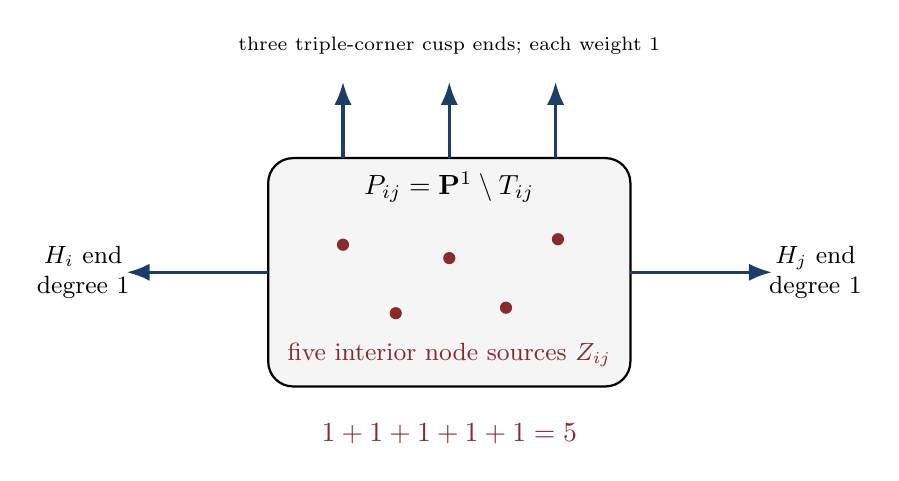
\begin{tikzpicture}[x=1cm,y=1cm,>=Latex,font=\small]
  \draw[rounded corners=9pt,thick,fill=softgray] (-2.3,-1.45) rectangle (2.3,1.45);
  \node[font=\bfseries] at (0,1.08) {$P_{ij}=\PP^1\setminus T_{ij}$};
  \foreach \x/\y in {-1.35/0.35,-0.68/-0.52,0/0.18,0.72/-0.45,1.38/0.42}
    \fill[deepred] (\x,\y) circle (2.2pt);
  \node[deepred] at (0,-1.05) {five interior node sources $Z_{ij}$};
  \draw[->,very thick,deepblue] (-2.3,0)--(-4.1,0);
  \draw[->,very thick,deepblue] (2.3,0)--(4.1,0);
  \node[align=center] at (-4.65,0) {$H_i$ end\\degree $1$};
  \node[align=center] at (4.65,0) {$H_j$ end\\degree $1$};
  \draw[->,very thick,deepblue] (-1.35,1.45)--(-1.35,2.42);
  \draw[->,very thick,deepblue] (0,1.45)--(0,2.42);
  \draw[->,very thick,deepblue] (1.35,1.45)--(1.35,2.42);
  \node[align=center,font=\scriptsize] at (0,2.88)
    {three triple-corner cusp ends; each weight $1$};
  \node[deepred,font=\bfseries] at (0,-2.05) {$1+1+1+1+1=5$};
\end{tikzpicture}
\caption{一つのdouble lineに対応するbalanced charge bookkeeping。二つのhorizontal arrowsは$N_{L/H_i}$と$N_{L/H_j}$のcurvature units、三つのvertical arrowsは\cref{cor:analytic-charge}のunit cusp fluxesを表す。五つのinterior sourcesとの関係は$5=2+3$である。}
\label{fig:punctured-neck-charge}
\end{figure}

\subsection{一般の$d$平面退化とquinticの特別性}

同じ計算はdegree-$d$ surfaceが一般位置の$d$平面へ退化する場合にも成立する。double line上のtriple pointsは$d-2$個、一般のsmoothing polynomialのzerosは$d$個である。

\begin{proposition}[degree-$d$ charge identity]\label{prop:degree-d-charge}
一般位置の$d$平面の和へ退化するdegree-$d$ surfaceについて、各double line $L$上で
\[
 \mathcal T^1|_L\cong\mathcal O_{\PP^1}(d),
 \qquad
 1+1+(d-2)-d=0.
\]
一方
\[
 K_L(T)\cong\mathcal O_{\PP^1}(d-4).
\]
従ってnormal bundle $N_{L/H}\cong\mathcal O(1)$とlog canonical bundle $K_L(T)$が一致するのは$d=5$に限る。
\end{proposition}

\begin{proof}
$N_{L/H}$は常に$\mathcal O(1)$、$\deg T=d-2$である。従って
$\mathcal T^1|_L\cong\mathcal O(1+1+d-2)=\mathcal O(d)$であり、smoothing polynomialのrestrictionは$\mathcal O(d)$のsectionである。また$\deg K_L(T)=-2+(d-2)=d-4$である。
\end{proof}

この意味でquinticは単に最小のcanonically polarized hypersurfaceであるだけでなく、double-stratum normal geometryとpair-of-pants log canonical geometryが同じline bundleで測られる唯一のdegreeである。

\subsection{Mandel neckとの比較：compact baseからthree-cusp baseへ}

Mandelのreduced KE equationは、compact negative curve $D$上でsingular $S^1$ fibrationを考え、point sourcesを含む形で
\begin{equation}\label{eq:mandel-reduced}
 \partial_z^2\chi+\Delta_D h=2\pi\sum_a\delta_{(q_a,0)}
\end{equation}
を解く。sourceはcircle bundle degreeのjumpを担い、局所rescalingにはTaub--NUT metricが現れる\cite{Mandel}。同論文はcompact base上で複数sourcesを加える場合もlinearized solutionsの重ね合わせで扱えることを明記している。従って新しい障害は``5点あること''ではなく、baseがthree-cusped noncompact surfaceであることと、三つのendsをtriple cornersへ同時にglueすることである。

本例で自然なbaseは$D=P_{ij}$であり、compactではない。従って必要なmodel problemは
\begin{equation}\label{eq:punctured-mandel-equation}
 \partial_z^2\chi+\Delta_{P_{ij}}h
 =2\pi\sum_{a=1}^{5}\delta_{(q_{ij,a},0)}
\end{equation}
に、次のend conditionsを課すことである。
\begin{enumerate}[label=(E\arabic*),leftmargin=3em]
\item $z$の両端で$H_i,H_j$側のlog-Calabi endsへmatchingする。
\item $P_{ij}$の三つのhyperbolic cusp endsでsource-free asymptoticsを持つ。
\item 各cusp endは対応するtriple pointの$C_3$ corner modelへ、他の二本のdouble neckと同時にmatchingする。
\end{enumerate}

\begin{question}[logarithmic Mandel neck]\label{q:log-mandel}
五点源を持つthree-cusped pair of pants上で、\eqref{eq:punctured-mandel-equation}をleading equationとするnegative KE neckを構成し、三つのcusp endsでuniform weighted Schauder estimatesを証明できるか。
\end{question}

compact-base caseとの主要な違いは、$\Delta_{P_{ij}}$がcusp spectrumとend modesを持つこと、三つのend dataが独立ではなくtriple-corner gluingでcoupleすること、global potential normalizationが10本のneck間で共有されることである。\cref{thm:balanced-five-source}はbase Poincar\'e--Lelong charge sectorを解き、三つのlinear cusp slopesをすべて$1$に固定した。さらに後述の\cref{thm:global-scalar-matching}はactual smoothing sectionに付随するbalanced real scalar corner classを消す。Mandelの$z$依存linearized operatorのweighted $L^2$ sector、complex scalar matching、filtered defect tower（第一対数層は8-dimensional）は後節で解決する。さらに\cref{sec:gamma2-scattering}では$P\cong\Gamma(2)\backslash\mathbb H$のexact scatteringを用い、punctured-neck側のstandard/common Laurent--Jordan transferをeven/odd両parityで任意の有限logarithmic orderまで決定する。従って残るlocal problemは、$\theta$-zeroのweighted Hölder--Zygmund/polyhomogeneous upgrade、triple-corner側のregular filtered channel matrices、regular scale-channel modulation、Taub--NUT source cores、およびnonlinear correctionである。nonzero angular modesは\cref{prop:angular-agmon}によりrapidly decaying sectorへ入る。

\subsection{punctured Mandel operatorのexact Pöschl--Teller因子分解}
\label{subsec:mandel-factorization}

Mandelのlinearized longitudinal operatorを、$T$に依存しない形へscaleする。$w=Tz$と置き、
\begin{equation}\label{eq:scaled-mandel-operator}
 \mathscr L_P
 =(1+w^2)\partial_w^2+6w\partial_w+4+\Delta_P
\end{equation}
とする。ここでも$\Delta_P\le0$である。自然なHilbert spaceは
\begin{equation}\label{eq:mandel-weighted-Hilbert}
 \mathscr H
 =L^2\!\left(\RR_w\times P,
 (1+w^2)^2\,dw\,dA_P\right)
\end{equation}
である。実際、$w$方向のprincipal partは
\[
 (1+w^2)\partial_w^2+6w\partial_w
 =(1+w^2)^{-2}\partial_w\bigl((1+w^2)^3\partial_w\bigr)
\]
とdivergence formに書ける。

\begin{theorem}[exact Pöschl--Teller factorization]\label{thm:mandel-factorization}
$w=\sinh s$、$c(s)=\cosh s$とし、
\[
 (Uf)(s,x)=c(s)^{5/2}f(\sinh s,x)
\]
と置く。$U:\mathscr H\to L^2(\RR_s\times P,ds\,dA_P)$はunitaryであり、
\begin{equation}\label{eq:mandel-unitary-factorization}
 -U\mathscr L_PU^{-1}
 =A+B,
 \qquad
 B=-\Delta_P,
\end{equation}
ただし
\begin{equation}\label{eq:poschl-teller-A}
 A=-\partial_s^2+\frac94-\frac{15}{4}\operatorname{sech}^2s
 =Q^*Q,
 \qquad
 Q=\partial_s+\frac32\tanh s.
\end{equation}
さらに
\begin{equation}\label{eq:A-spectrum}
 \sigma(A)=\{0,2\}\cup[9/4,\infty),
 \qquad
 \ker A=\RR\operatorname{sech}^{3/2}s.
\end{equation}
従って
\begin{equation}\label{eq:mandel-kernel}
 \ker_{\mathscr H}\mathscr L_P
 =\RR\,(1+w^2)^{-2}\otimes1_P.
\end{equation}
$\lambda_P=\inf(\sigma(B)\setminus\{0\})>0$とすると、上のkernelの直交補空間で
\begin{equation}\label{eq:mandel-gap}
 \langle-\mathscr L_Pf,f\rangle_{\mathscr H}
 \ge \min\{2,\lambda_P\}\,\|f\|_{\mathscr H}^2
\end{equation}
が成り立つ。
\end{theorem}

\begin{proof}
$dw=c(s)ds$かつ$(1+w^2)^2=c(s)^4$なので
\[
 (1+w^2)^2|f(w,x)|^2dw
 =|c(s)^{5/2}f(\sinh s,x)|^2ds,
\]
従って$U$はunitaryである。$f=c^{-5/2}y$を直接微分すると
\begin{equation}\label{eq:conjugation-calculation}
 \bigl((1+w^2)\partial_w^2+6w\partial_w+4\bigr)f
 =c^{-5/2}
 \left(\partial_s^2-\frac94+\frac{15}{4}\operatorname{sech}^2s\right)y.
\end{equation}
$P$方向のLaplacianは$c$と可換なので\eqref{eq:mandel-unitary-factorization}を得る。また
\[
 Q^*Q
 =\left(-\partial_s+\frac32\tanh s\right)
  \left(\partial_s+\frac32\tanh s\right)
 =A.
\]
spectrumもfactorizationだけから確認できる。$Q_\ell=\partial_s+\ell\tanh s$、$A_\ell=Q_\ell^*Q_\ell$と置くと
\[
 A_\ell=-\partial_s^2+\ell^2-\ell(\ell+1)\operatorname{sech}^2s,
 \qquad
 Q_\ell Q_\ell^*=A_{\ell-1}+2\ell-1.
\]
$\ell=1/2$では$Q_{1/2}Q_{1/2}^*=-\partial_s^2+1/4+(1/4)\operatorname{sech}^2s\ge1/4$である。従って$A_{1/2}$はzero mode $\operatorname{sech}^{1/2}s$以外に$1/4$未満のspectrumを持たず、essential spectrumは$[1/4,\infty)$である。さらに
\[
 Q_{3/2}Q_{3/2}^*=A_{1/2}+2
\]
なので、$A=A_{3/2}$のnonzero spectrumは$\{2\}\cup[9/4,\infty)$となる。zero modeは$Q_{3/2}y=0$の解$y=\operatorname{sech}^{3/2}s$であり、\eqref{eq:A-spectrum}を得る。$P$はfinite-area connected hyperbolic surfaceなので、$B$のzero eigenspaceはconstantsであり、その直交補空間のspectrumは$\lambda_P>0$以上にある。$A+B$のspectral decompositionから\eqref{eq:mandel-kernel},\eqref{eq:mandel-gap}を得る。
\end{proof}

\begin{remark}[continuous spectrumは$L^2$ obstructionではない]\label{rem:continuous-spectrum-solved}
$P$の$L^2$ spectrumには、有限個のdiscrete spectrumに加えて$[1/4,\infty)$から始まるcontinuous spectrumがある\cite{Iwaniec}。しかし\cref{thm:mandel-factorization}はpoint spectrumとcontinuous spectrumを区別せず、spectral measure全体に対して$A+B$のnonnegativityとkernelを決定する。従ってcontinuous spectrumそのものはweighted $L^2$ invertibilityの障害ではない。Mandelのhypergeometric representationで特定parameterにchosen pair of solutionsが退化する現象も、operatorの新しいkernelを意味しない。残る問題は、prescribed non-$L^2$ cusp asymptoticsを含むweighted Hölder/polyhomogeneous mapping propertyである。
\end{remark}

\subsection{positive spectral Green multiplierと一階gain}

$\lambda>0$に対し、$m_\lambda$を
\begin{equation}\label{eq:green-multiplier-ode}
 (1+w^2)m_\lambda''+6wm_\lambda'
 +(4-\lambda^2)m_\lambda
 =2\pi\delta_0
\end{equation}
の両端でdecayするeven solutionとする。\cref{thm:mandel-factorization}により一意に定まる。

\begin{proposition}[high-frequency Green bound]\label{prop:green-multiplier}
$\lambda>2$なら$m_\lambda\le0$であり、
\begin{equation}\label{eq:green-high-frequency-bound}
 \sup_{w\in\RR}|m_\lambda(w)|
 =-m_\lambda(0)
 \le \frac{\pi}{\sqrt{\lambda^2-4}}.
\end{equation}
さらに$P$のpositive spectrum上では、ある$C_P>0$が存在して
\begin{equation}\label{eq:green-order-minus-one}
 \sup_{w\in\RR}|m_\lambda(w)|
 \le \frac{C_P}{1+\lambda}
 \qquad
 (\lambda^2\in\sigma(-\Delta_P)\setminus\{0\}).
\end{equation}
\end{proposition}

\begin{proof}
$u=-m_\lambda$、$a=\sqrt{\lambda^2-4}$と置く。\eqref{eq:green-multiplier-ode}を$(1+w^2)^2$倍すると
\[
 -\partial_w\bigl((1+w^2)^3u'\bigr)
 +a^2(1+w^2)^2u=2\pi\delta_0.
\]
maximum principleから$u\ge0$であり、最大値は$w=0$で取る。$u$を掛けて積分すると
\begin{equation}\label{eq:green-energy}
 \int_{\RR}(1+w^2)^3|u'|^2dw
 +a^2\int_{\RR}(1+w^2)^2u^2dw
 =2\pi u(0).
\end{equation}
一方、半直線上のtrace inequalityを両側へ適用して
\[
 \int_{\RR}(|u'|^2+a^2u^2)dw\ge2a\,u(0)^2.
\]
\eqref{eq:green-energy}の左辺はこれ以上なので、$u(0)\le\pi/a$を得る。これが\eqref{eq:green-high-frequency-bound}である。positive spectrumのうちbounded intervalにある部分では、$A+\lambda^2$のresolvent kernelが$\lambda>0$に連続に依存し、$\lambda\ge\sqrt{\lambda_P}$である。これとhigh-frequency boundを合わせて\eqref{eq:green-order-minus-one}を得る。
\end{proof}

$B=-\Delta_P$とし、$H_B^s(P)=\operatorname{Dom}(1+B)^{s/2}$をspectral Sobolev spaceとする。$\Pi_0$をconstantsへのorthogonal projectionとする。spectral functional calculusにより
\[
 \mathcal M_w=m_{\sqrt B}(w)(1-\Pi_0)
\]
を定義する。

\begin{corollary}[mean-zero sectorの一階gain]\label{cor:mandel-one-derivative-gain}
任意の$s\in\RR$に対し
\begin{equation}\label{eq:mandel-sobolev-gain}
 \sup_{w\in\RR}
 \|\mathcal M_wF\|_{H_B^{s+1}(P)}
 \le C_s\|F\|_{H_B^s(P)},
 \qquad \Pi_0F=0.
\end{equation}
元の$z$ coordinateでは
\[
 u_T(z,\cdot)=T\mathcal M_{Tz}F
\]
が
\[
 \bigl((z^2+T^{-2})\partial_z^2+6z\partial_z+4+\Delta_P\bigr)u_T
 =2\pi\delta_0(z)F
\]
を満たし、$T^{-1}u_T$に対する\eqref{eq:mandel-sobolev-gain}は$T$に一様である。
\end{corollary}

\begin{proof}
\eqref{eq:green-order-minus-one}は$\lambda$に関するorder $-1$ multiplier estimateである。spectral theoremを適用すれば\eqref{eq:mandel-sobolev-gain}を得る。$w=Tz$では$\delta_0(w)=T^{-1}\delta_0(z)$なので、$T m_{\sqrt B}(Tz)$が正しいrescalingである。
\end{proof}

\subsection{linearized five-source equationの明示解}

$\delta_Z=\sum_{a=1}^5\delta_{q_a}$とし、$\operatorname{Area}(P)=2\pi$を用いて
\begin{equation}\label{eq:source-mean-zero-decomposition}
 F_Z=\delta_Z-\frac5{2\pi}\,1_P,
 \qquad \Pi_0F_Z=0
\end{equation}
と置く。base constant modeのGreen profileは
\begin{equation}\label{eq:m0-explicit}
 m_0(w)
 =\pi\frac{|w|+|w|^3/3}{(1+w^2)^2}.
\end{equation}
これは$w\ne0$でhomogeneous equationを満たし、$m_0'(0+)-m_0'(0-)=2\pi$なので
\[
 \bigl((1+w^2)\partial_w^2+6w\partial_w+4\bigr)m_0
 =2\pi\delta_0.
\]

\begin{theorem}[linear five-source solution]\label{thm:linear-five-source}
分布方程式
\begin{equation}\label{eq:linear-five-source-equation}
 \mathscr L_Pu
 =2\pi\delta_0(w)\delta_Z
\end{equation}
は
\begin{equation}\label{eq:linear-five-source-solution}
 u_Z(w,\cdot)
 =\frac5{2\pi}m_0(w)
 +\mathcal M_wF_Z
 +c(1+w^2)^{-2},
 \qquad c\in\RR,
\end{equation}
により解かれる。最後の項は唯一のweighted $L^2$ kernelである。任意の$\eps>0$について$F_Z\in H_B^{-1-\eps}(P)$なので、mean-zero partは各$w$で$H_B^{-\eps}(P)$に属し、sourcesを除けばsmoothである。
\end{theorem}

\begin{proof}
\eqref{eq:source-mean-zero-decomposition}をconstant partとmean-zero partへ代入する。第一項は\eqref{eq:m0-explicit}からconstant part$5\delta_0$を与え、第二項はspectral theoremと\eqref{eq:green-multiplier-ode}から$2\pi\delta_0F_Z$を与える。\cref{thm:mandel-factorization}によりhomogeneous weighted $L^2$ freedomは最後の一項だけである。二次元のDirac massのSobolev regularityと\cref{cor:mandel-one-derivative-gain}から最後のregularity statementが従う。
\end{proof}

\begin{remark}
$m_0(w)\sim\pi/(3|w|)$であり、\eqref{eq:mandel-weighted-Hilbert}には属さない。これは欠陥ではなく、二つのcomponent endsのcircle-bundle degreeを変えるtopological constant modeである。したがってlinear problemの正しい分解は、decaying $L^2$ sectorと、明示的なnon-$L^2$ topological modesを最初から分けることである。
\end{remark}


\subsection{Mandel零モードのscale--degree辞書と五点源jump}
\label{subsec:scale-degree-dictionary}

Mandelの$D$方向にconstantなreduced familyは
\begin{equation}\label{eq:exact-mandel-two-parameter-family}
 \chi_{\alpha}(z)=1+\alpha z,
 \qquad
 h_{\alpha,T}(z)
 =\frac{1+\alpha z}
 {z^2+\frac23\alpha z^3+T^{-2}}
\end{equation}
であり、sourceから離れた領域で
\begin{equation}\label{eq:exact-mandel-reduced-ode}
 \partial_z\bigl(\log h_{\alpha,T}-\log\chi_\alpha\bigr)
 =-2h_{\alpha,T}z
\end{equation}
をexactに満たす\cite{Mandel}。この二parameter familyを微分すると、\eqref{eq:longitudinal-zero-modes}の二つの零モードの幾何学的意味が完全に決まる。

\begin{proposition}[scale--degree dictionary]\label{prop:scale-degree-dictionary}
$w=Tz$とする。微分はまず$z$を固定して行い、その後$z=w/T$を代入する。このとき
\begin{equation}\label{eq:u0-scale-derivative}
 \left.
 \frac1{2T^2}\,\partial_{\log T}h_{0,T}(z)
 \right|_{z=w/T}
 =u_0(w),
\end{equation}
\begin{equation}\label{eq:u1-degree-derivative}
 \left.
 \frac1T\,\partial_{\alpha}h_{\alpha,T}(z)
 \right|_{\alpha=0,\ z=w/T}
 =u_1(w).
\end{equation}
従って$u_0$はneck scale $\log T$のJacobi field、$u_1$は二つのCalabi endsのdegree/asymmetry parameterのJacobi fieldである。
\end{proposition}

\begin{proof}
$h_{0,T}=(z^2+T^{-2})^{-1}$を直接微分すれば
\[
 \partial_{\log T}h_{0,T}
 =\frac{2T^{-2}}{(z^2+T^{-2})^2},
\]
従って\eqref{eq:u0-scale-derivative}を得る。また\eqref{eq:exact-mandel-two-parameter-family}を$\alpha$で微分して$\alpha=0$、$z=w/T$を代入すると
\[
 T^{-1}\partial_\alpha h_{\alpha,T}|_{\alpha=0,z=w/T}
 =\frac{w+w^3/3}{(1+w^2)^2}
 =u_1(w).
\]
Mandel modelでは$\chi=1+k_\pm z+O(T^{-1})$のslope $k_\pm$が両端のcircle-bundle degreeを与えるので、後半の解釈も従う\cite{Mandel}。
\end{proof}

\begin{proposition}[五点源のexact topological jump]\label{prop:five-source-degree-jump}
\cref{thm:linear-five-source}のsolutionに任意のhomogeneous topological mode$b u_1$を加える。$w\ne0$では
\begin{equation}\label{eq:m0-sign-u1}
 m_0(w)=\pi\,\operatorname{sgn}(w)u_1(w)
\end{equation}
であり、base constant projectionは
\begin{equation}\label{eq:five-source-base-average}
 \Pi_0\bigl(u_Z+b u_1\bigr)
 =\left(b+\frac52\operatorname{sgn}(w)\right)u_1(w)
 +c u_0(w).
\end{equation}
従って両component endsにおける$u_1$ coefficientを$a_+,a_-$とすると
\begin{equation}\label{eq:degree-jump-five}
 a_+-a_-=5.
\end{equation}
このjumpは五点の位置には依存せず、source divisorのdegreeだけで決まる。
\end{proposition}

\begin{proof}
\eqref{eq:m0-explicit}と$u_1$の定義から\eqref{eq:m0-sign-u1}は直ちに従う。mean-zero multiplierは$\Pi_0\mathcal M_wF_Z=0$を満たすので、\eqref{eq:linear-five-source-solution}のconstant projectionは\eqref{eq:five-source-base-average}である。$w>0$と$w<0$の係数を引けば\eqref{eq:degree-jump-five}を得る。
\end{proof}

\begin{remark}[相対degree jumpとcusp flux]\label{rem:odd-degree-affine-line}
五点源はodd homogeneous modeを任意に生成するのではなく、二端の$u_1$ coefficientsの\emph{差}を$5$に固定する。残るhomogeneous自由度は平均$(a_++a_-)/2=b$だけである。ただし$P$は三つのcuspを持つnoncompact baseなので、$a_\pm$をcompact-base Mandel modelのabsolute bundle degreesと無修正に同一視してはならない。これらはcusp trivializationsを固定した\emph{relative degree coefficients}であり、global normal-bundle bookkeepingでは三つのunit cusp fluxを差し引いて
\[
 5=\underbrace{(1+1)}_{\text{two component normal units}}
   +\underbrace{(1+1+1)}_{\text{three corner fluxes}}
\]
と読むべきである。従ってodd sectorのglobal problemはsource jumpそのものではなく、平均degree/asymmetryと三つのcorner gaugesを整合させる問題である。
\end{remark}

\begin{corollary}[balanced referenceにおけるodd centering]\label{cor:balanced-odd-centering}
centered longitudinal coordinateを用い、\cref{thm:linear-five-source}のnormalized particular solutionを選ぶと、そのhomogeneous coefficientは$b=0$である。従ってreference five-source neckの二端係数は
\[
 a_+=\frac52,\qquad a_-=-\frac52,
\]
であり、平均degree/asymmetryは$0$にcenterされる。このstatementはsource divisorの位置に依存しない。
\end{corollary}

\begin{proof}
\cref{prop:source-even-parity}の通りnormalized particular solutionは$w\mapsto-w$でevenである。$u_1$はoddなのでhomogeneous term$b u_1$はこのnormalizationでは現れず、\eqref{eq:five-source-base-average}で$b=0$となる。
\end{proof}


\subsection{第一対数層とfiltered polyhomogeneous defect tower}
\label{subsec:corrected-defect-block}

前版では、幾何学的に必要と考えられる$1,r,\log r$型の解だけを取り出し、それを``exact six-dimensional defect block''と呼んだ。v0.8では$r\log r$型を加えて8-dimensional blockへ訂正したが、なお``complete low-growth block''という呼称は強すぎる。実際、parameter-dependent indicial solutionsを高階微分すれば、root-$0$側に任意次数の$(\log r)^n$が現れ、これらはすべて$r\log r$より遅くしか増大しない。一方、root-$1$側の$r(\log r)^n$は$n\ge2$でこのgrowth boundを越える。本節では、まずlog-degree $\le1$の第一対数層を厳密に記述し、その後に全filtered towerを構成する。

longitudinal homogeneous solutionsを
\begin{equation}\label{eq:longitudinal-zero-modes}
 u_0(w)=\frac1{(1+w^2)^2},
 \qquad
 u_1(w)=\frac{w+w^3/3}{(1+w^2)^2}
\end{equation}
とする。これらは$H_0u_i=0$を満たし、Wronskianは$(1+w^2)^{-3}$である。Jordan partnersを次のexplicit functionsで固定する：
\begin{equation}\label{eq:jordan-v0}
 v_0(w)=
 \frac{w^3\arctan w+w^2+3w\arctan w-\log(1+w^2)+2}
 {6(1+w^2)^2},
\end{equation}
\begin{equation}\label{eq:jordan-v1}
 v_1(w)=
 \frac{-2w^3+3w(w^2+3)\log(1+w^2)-30w+12\arctan w}
 {54(1+w^2)^2}.
\end{equation}
直接計算により$H_0v_i=u_i$である。

\begin{proposition}[第一対数層]\label{prop:cusp-defect-block}
\[
 H_0=(1+w^2)\partial_w^2+6w\partial_w+4
\]
とし、\eqref{eq:longitudinal-zero-modes}, \eqref{eq:jordan-v0}, \eqref{eq:jordan-v1}のfunctionsを用いる。$\mathscr W_1$を、$|w|\to\infty$で高々$O((1+\log\langle w\rangle)/\langle w\rangle)$の成長を持ち、同じ型の微分評価を満たすfunctionsのclassとする。このとき
\begin{equation}\label{eq:generalized-longitudinal-nullspace}
 \ker(H_0^2|_{\mathscr W_1})
 =\operatorname{span}\{u_0,u_1,v_0,v_1\},
 \qquad
 \ker(H_0|_{\mathscr W_1})
 =\operatorname{span}\{u_0,u_1\}.
\end{equation}
exact cusp metric
$g=(dr^2+d\theta^2)/r^2$上で、$\theta$に依存せず
\begin{equation}\label{eq:low-growth-ansatz}
 F(w,r)=A(w)r\log r+B(w)r+C(w)\log r+D(w),
 \qquad A,B,C,D\in\mathscr W_1
\end{equation}
という形を持つ$\mathscr L F=0$の解全体は、次の8 functionsで張られる：
\begin{equation}\label{eq:full-eight-defect-basis}
 \begin{aligned}
 &u_0r,\ u_1r,\quad u_0,\ u_1,\\
 &u_0\log r+v_0,\quad u_1\log r+v_1,\\
 &u_0r\log r-v_0r,\quad
 u_1r\log r-v_1r.
 \end{aligned}
\end{equation}
従ってansatz \eqref{eq:low-growth-ansatz}、すなわちlog-degree $\le1$の第一対数層の次元は$8$である。
\end{proposition}

\begin{proof}
$H_0$は二階常微分作用素なので$H_0^2F=0$の局所解空間は4次元である。$u_0,u_1,v_0,v_1$は線形独立で、$H_0u_i=0$, $H_0v_i=u_i$を満たすから\eqref{eq:generalized-longitudinal-nullspace}を得る。

cusp Laplacianの$\theta$-constant partは
\[
 \Delta_{\mathrm{cusp}}=r^2\partial_r^2,
\]
従って
\[
 \Delta r=0,\qquad
 \Delta\log r=-1,\qquad
 \Delta(r\log r)=r.
\]
\eqref{eq:low-growth-ansatz}を$\mathscr LF=0$へ代入し、$r\log r,r,\log r,1$の係数を比較すると
\begin{equation}\label{eq:defect-coefficient-system}
 H_0A=0,\qquad
 H_0B=-A,\qquad
 H_0C=0,\qquad
 H_0D=C.
\end{equation}
$V(u_i)=v_i$と書けば
\[
 A\in\ker H_0,\quad
 B=-V(A)+\ker H_0,\quad
 C\in\ker H_0,\quad
 D=V(C)+\ker H_0.
\]
これが\eqref{eq:full-eight-defect-basis}を与える。各basis elementが実際にkernelに入ることは直接計算でも確認できる。
\end{proof}

\begin{remark}[前版の6次元spaceの正しい意味]\label{rem:geometric-six-defect}
前版で用いた
\begin{equation}\label{eq:geometric-six-defect}
 \mathfrak D_{\mathrm{geom}}
 =\operatorname{span}\{u_0r,u_1r,u_0,u_1,
 u_0\log r+v_0,u_1\log r+v_1\}
\end{equation}
は、第一対数層$\mathfrak D_1$内のcodimension-$2$ subspaceである。これは``root-$1$ Jordan residueをゼロにする''というno-$r\log r$ normalizationで特徴付けられる。balanced static potentialとcanonical weighted $L^2$ correctionはこのnormalizationと整合するが、一般のpolyhomogeneous boundary problemでは最後の二モードを最初から排除してはならない。さらに高いlogarithmic orderでは後述のtower modesも加わるため、8次元space自体もfull trace spaceではない。
\end{remark}

\begin{remark}[parity]\label{rem:defect-parity}
$u_0,v_0$は$w\mapsto-w$でeven、$u_1,v_1$はoddである。従って8 modesは四つのeven modesと四つのodd modesに分かれる。neck orientationを反転したとき、even coefficientsは通常のscalar cochainsとして、odd coefficientsは後述のorientation local system $\mathfrak o_\Gamma$に値を持つcochainsとして変換する。
\end{remark}


\begin{theorem}[filtered defect tower]\label{thm:filtered-defect-tower}
$p\in\{0,1\}$とする。$s=1$の近傍で
\begin{equation}\label{eq:filtered-longitudinal-family}
 (H_0+s(s-1))U_s^{(p)}=0,
 \qquad
 U_1^{(p)}=u_p,
 \qquad
 \partial_sU_s^{(p)}|_{s=1}=-v_p
\end{equation}
を満たすanalytic ODE germを取る。$n\ge0$に対して
\begin{align}
 \mathsf T_{1,n}^{(p)}
 &:=\frac1{n!}
   \left.\partial_s^n\bigl(U_s^{(p)}r^s\bigr)\right|_{s=1},
 \label{eq:root-one-filtered-tower}\\
 \mathsf T_{0,n}^{(p)}
 &:=\frac1{n!}
   \left.\partial_\sigma^n
   \bigl(U_{1-\sigma}^{(p)}r^\sigma\bigr)
   \right|_{\sigma=0}.
 \label{eq:root-zero-filtered-tower}
\end{align}
このとき
\begin{equation}\label{eq:filtered-tower-kernel}
 \mathscr L\mathsf T_{\sigma,n}^{(p)}=0
 \qquad(\sigma=0,1)
\end{equation}
であり、最高log-degree項は
\begin{align}
 \mathsf T_{1,n}^{(p)}
 &=r\left(
   \frac{u_p}{n!}(\log r)^n
   +\text{lower log degree}
   \right),
 \label{eq:root-one-tower-leading}\\
 \mathsf T_{0,n}^{(p)}
 &=\frac{u_p}{n!}(\log r)^n
   +\text{lower log degree}.
 \label{eq:root-zero-tower-leading}
\end{align}
従って
\begin{equation}\label{eq:filtered-defect-space}
 \mathfrak D_N
 :=\operatorname{span}\left\{
 \mathsf T_{\sigma,n}^{(p)}:
 \sigma,p\in\{0,1\},\ 0\le n\le N
 \right\}
\end{equation}
は
\begin{equation}\label{eq:filtered-defect-dimension}
 \boxed{\dim\mathfrak D_N=4(N+1)}
\end{equation}
を満たし、$\mathfrak D_1$は\cref{prop:cusp-defect-block}の8-dimensional first layerに一致する。

さらに
\begin{equation}\label{eq:second-longitudinal-jordan}
 z_p:=\frac12\partial_s^2U_s^{(p)}|_{s=1}
\end{equation}
と置けば
\begin{equation}\label{eq:H0-zp}
 H_0z_p=v_p-u_p
\end{equation}
であり、second layerは
\begin{align}
 \mathsf T_{1,2}^{(p)}
 &=r\left(
 \frac12u_p(\log r)^2-v_p\log r+z_p
 \right),
 \label{eq:T12-explicit}\\
 \mathsf T_{0,2}^{(p)}
 &=\frac12u_p(\log r)^2+v_p\log r+z_p.
 \label{eq:T02-explicit}
\end{align}
analytic scalar gauge $U_s^{(p)}\mapsto a_p(s)U_s^{(p)}$は各$\mathfrak D_N$のbasisをupper triangularに変えるだけで、filtration自体を変えない。
\end{theorem}

\begin{proof}
ODEのanalytic parameter dependenceにより\eqref{eq:filtered-longitudinal-family}を満たすgermが存在する。$\mathscr L(U_s^{(p)}r^s)=0$および
$\mathscr L(U_{1-\sigma}^{(p)}r^\sigma)=0$をparameterで微分すれば
\eqref{eq:filtered-tower-kernel}を得る。Leibniz則から
\eqref{eq:root-one-tower-leading},
\eqref{eq:root-zero-tower-leading}が従う。root $0$とroot $1$、二つのparities、異なる最高log degreeを比較すればlinear independenceが従い、\eqref{eq:filtered-defect-dimension}を得る。

\eqref{eq:filtered-longitudinal-family}を二回微分して$s=1$を代入すると
\[
 H_0\partial_s^2U_s^{(p)}|_1
 +2\partial_sU_s^{(p)}|_1+2u_p=0.
\]
$\partial_sU_s^{(p)}|_1=-v_p$を用いれば
\eqref{eq:H0-zp}を得る。Leibniz則をもう一度用いれば
\eqref{eq:T12-explicit},\eqref{eq:T02-explicit}となる。gauge statementもLeibniz則から明らかである。
\end{proof}

\begin{remark}[finite-dimensionalなのは各filtered layerである]\label{rem:no-complete-low-growth-block}
任意の$n$についてroot-$0$ mode $(\log r)^n=o(r\log r)$である。従って成長条件$O(r\log r)$だけでpolyhomogeneous kernelを有限次元にすることはできない。解析上正しい対象は、許すlogarithmic orderを固定したfiltered space$\mathfrak D_N$である。非線形iterationの各段階では必要な$N$だけをadjoinし、remainderをweighted spaceへ入れるべきである。
\end{remark}

\begin{proposition}[root-$1$ resonance audit]\label{prop:root-one-resonance-audit}
$q(w)=(1+w^2)^2$とし、$\langle f,g\rangle_q=\int_{\RR}fgq\,dw$と書く。$G\in L^2(\RR,q\,dw)$に対し、exact cusp上で
\begin{equation}\label{eq:resonant-inhomogeneous-expansion}
 \mathscr L F=rG(w)+o(r),
 \qquad
 F=r\log r\,A(w)+rB(w)+o(r)
\end{equation}
とする。$A\in\ker H_0\cap L^2(q\,dw)$、$B\in\operatorname{Dom}H_0$ならば
\begin{equation}\label{eq:root-one-residue-formula}
 A=a_0u_0,
 \qquad
 a_0
 =\frac{\langle G,u_0\rangle_q}{\|u_0\|_q^2}
 =\frac{2}{\pi}\int_{\RR}G(w)\,dw.
\end{equation}
従ってHilbert-even channelに$r\log r$ termが現れないための必要十分条件は
\begin{equation}\label{eq:no-rlog-moment-condition}
 \int_{\RR}G(w)\,dw=0
\end{equation}
である。特に$G=\partial_wJ$で$J(+\infty)=J(-\infty)$ならroot-$1$ residueは消える。
\end{proposition}

\begin{proof}
$\Delta_{\mathrm{cusp}}(r\log r)=r$、$\Delta_{\mathrm{cusp}}r=0$なので、\eqref{eq:resonant-inhomogeneous-expansion}の$r$係数を比較すると
\[
 A+H_0B=G.
\]
$H_0$は$L^2(q\,dw)$でself-adjointであり、Hilbert kernelは$\RR u_0$である。従って$u_0$とpairingして
\[
 a_0\|u_0\|_q^2=\langle G,u_0\rangle_q.
\]
一方
\[
 q u_0=1,
 \qquad
 \|u_0\|_q^2
 =\int_{\RR}\frac{dw}{(1+w^2)^2}
 =\frac\pi2,
\]
なので\eqref{eq:root-one-residue-formula}を得る。最後の主張は積分による。
\end{proof}

\begin{remark}[root-$1$ momentはscale-channel modulation equationである]\label{rem:resonance-audit-meaning}
\cref{prop:scale-degree-dictionary}により$u_0$は$\log T$のJacobi fieldである。従って\cref{prop:root-one-resonance-audit}のmoment
\[
 \frac2\pi\int_{\RR}G(w)\,dw
\]
は、単に``消えるべきerror''ではなく、neckの\emph{scale channel}へのLyapunov--Schmidt obstructionである。ただしroot-$1$ modeは$r u_0$であり、これはconstantな$T$ shiftだけではなく、cusp depthに依存するscale correctionを表す。従ってactual gluingでは、root-$0$のrelative shifts（bounded、少なくともsublinearであることを示すべき未知量）とroot-$1$以上のfiltered cusp-dependent scale tracesをまとめてcorner dataへ加え、projected equationsから決めるべきである。

scale channelをあらかじめ消したgaugeでは\eqref{eq:no-rlog-moment-condition}を課す必要がある。errorが$w$方向divergenceならこのgaugeでmomentは自動消滅するが、一般にはtriple-corner filtered Calder\'on mapとのmatching equationになる。\cref{prop:scale-modulation-invisible}により、得られるlog-scale correctionが全overlapで$o(R_t)$ならfirst-scale cubical limitと$\sqrt{13}$ coefficientは変わらない。従って主予想のために必要なのは各momentの個別消滅より弱く、scale-channel correction全体のsublinear controlである。nonlinear proofで必要なのは、global common leading scaleを$t$で固定した後のregular scale-channel matrixがinvertibleであることと、odd $u_1$ average modesを\cref{prop:five-source-degree-jump}のfixed jumpと両立させることである。
\end{remark}

\subsection{Mellin indicial familyとroot-free spectral window}
\label{subsec:indicial-family}

exact cuspで$y=\log r$と置く。$\theta$-zero modeに対して
\[
 -\Delta_P=-\partial_y^2+\partial_y.
\]
$e^{\sigma y}=r^\sigma$を代入したindicial familyは
\begin{equation}\label{eq:indicial-family-original}
 I(\sigma)=H_0+\sigma(\sigma-1).
\end{equation}
\cref{thm:mandel-factorization}の$w$方向unitary map $U$を用いると
\begin{equation}\label{eq:indicial-family-A}
 -UI(\sigma)U^{-1}=A-\sigma(\sigma-1).
\end{equation}

\begin{theorem}[Hilbert-sector indicial spectrum]\label{thm:indicial-spectrum}
$A$のspectrumは$\{0,2\}\cup[9/4,\infty)$である。従ってweighted Hilbert sectorのindicial exponentsは
\begin{equation}\label{eq:indicial-root-set}
 \{0,1,-1,2\}
 \cup
 \left(-\infty,\frac{1-\sqrt{10}}2\right]
 \cup
 \left[\frac{1+\sqrt{10}}2,\infty\right).
\end{equation}
特に
\begin{equation}\label{eq:root-free-strips}
 (-1,0),\qquad(0,1),\qquad(1,2)
\end{equation}
はroot-freeである。$\mu=2$に対応するlongitudinal profileは、定数倍を除いて
\begin{equation}\label{eq:mu2-profile}
 h_2(w)=\frac{w}{(1+w^2)^2},
 \qquad H_0h_2=-2h_2
\end{equation}
である。非Hilbert zero resonance $u_1$は$\sigma=0,1$にもう一つのcopyを加えるが、新しいexponentは作らない。
\end{theorem}

\begin{proof}
\eqref{eq:indicial-family-A}から、Hilbert-sector indicial equationは
\[
 \sigma(\sigma-1)=\mu,
 \qquad \mu\in\sigma(A)
\]
である。$\mu=0$から$\sigma=0,1$、$\mu=2$から$\sigma=-1,2$を得る。$\mu\ge9/4$に対する二根は
\[
 \sigma_\pm(\mu)=\frac{1\pm\sqrt{1+4\mu}}2
\]
であり、その端点が$(1\pm\sqrt{10})/2$である。\eqref{eq:mu2-profile}は直接微分、またはPöschl--Tellerの第一励起状態
$\tanh s\,\operatorname{sech}^{1/2}s$を$w$へ戻すことで得られる。$u_1$は$H_0u_1=0$を満たすが\eqref{eq:mandel-weighted-Hilbert}には属さないため、Hilbert spectrumではなく明示的topological defectとして加える。
\end{proof}

\begin{remark}[なぜ$8$次元で止められるか]
$\mu=2$の次のpositive indicial exponentは$(1+\sqrt{10})/2>2$である。従ってgrowth $O(r\log r)$までに現れ得るindicial rootsは$\sigma=0,1$だけである。ただし各rootのparameter derivativesから任意次数のlogarithmic towerが生じるため、このgrowth条件だけでkernelが有限次元になるわけではない。$r^2h_2$やcontinuous-spectrum exponentsは次のpower-growth tierに属する。
\end{remark}

\subsection{exact cuspにおけるcentral-strip coercivity}
\label{subsec:weighted-cusp-coercivity}

$y=\log r$とし、$w$方向のunitary mapに加えてbase density conjugationを行う：
\begin{equation}\label{eq:double-unitary-map}
 (\mathcal U f)(s,y,\theta)
 =e^{-y/2}(\cosh s)^{5/2}
 f(\sinh s,e^y,\theta).
\end{equation}
するとnatural $L^2$ measureは$ds\,dy\,d\theta$となる。

\begin{theorem}[exact weighted end identity]\label{thm:weighted-end-identity}
exact hyperbolic cusp上で
\begin{equation}\label{eq:exact-cusp-conjugated-operator}
 -\mathcal U\mathscr L\mathcal U^{-1}
 =\mathcal K
 :=A-\partial_y^2+\frac14-e^{2y}\partial_\theta^2.
\end{equation}
$\delta\in\RR$とし
\[
 \mathcal K_\delta=e^{\delta y}\mathcal K e^{-\delta y}
\]
と置く。compactly supported smooth $v$に対して
\begin{equation}\label{eq:central-strip-energy-identity}
 \begin{aligned}
 \operatorname{Re}\langle\mathcal K_\delta v,v\rangle
 ={}&\langle Av,v\rangle
 +\|\partial_yv\|^2
 +\|e^y\partial_\theta v\|^2\\
 &+\left(\frac14-\delta^2\right)\|v\|^2.
 \end{aligned}
\end{equation}
従って$|\delta|<1/2$ならexact end normal operatorはcoerciveであり、
\begin{equation}\label{eq:central-strip-L2-bound}
 \|v\|_{L^2}
 \le
 \left(\frac14-\delta^2\right)^{-1}
 \|\mathcal K_\delta v\|_{L^2}
\end{equation}
を満たす。
\end{theorem}

\begin{proof}
$-\Delta_P=-\partial_y^2+\partial_y-e^{2y}\partial_\theta^2$であり、$e^{-y/2}$ conjugationにより$-\partial_y^2+1/4-e^{2y}\partial_\theta^2$となる。これと\cref{thm:mandel-factorization}を合わせて\eqref{eq:exact-cusp-conjugated-operator}を得る。さらに
\[
 \mathcal K_\delta
 =A-(\partial_y-\delta)^2+\frac14-e^{2y}\partial_\theta^2.
\]
$2\delta\partial_y$のreal partはゼロであり、部分積分により\eqref{eq:central-strip-energy-identity}を得る。$A\ge0$なので\eqref{eq:central-strip-L2-bound}が従う。
\end{proof}

\begin{remark}
式\eqref{eq:central-strip-energy-identity}は、base cuspのcontinuous threshold $1/4$がPöschl--Teller operatorのnonnegativityと正確に加算されることを示す。中央のweight window $|\delta|<1/2$は、元のindicial exponentで$0<\operatorname{Re}\sigma<1$に対応し、\cref{thm:indicial-spectrum}のroot-free stripと一致する。
\end{remark}

\begin{proposition}[global weighted Hilbert Fredholm theorem]\label{prop:global-weighted-Hilbert-parametrix}
$P=\PP^1\setminus\{0,1,\infty\}$にcomplete hyperbolic metricを入れる。各cuspで$y$に等しくcompact coreで一定となるsmooth function $\varpi$を取り、
\[
 W_\delta=e^{\delta\varpi},
 \qquad
 \mathcal H^m_\delta
 =W_\delta^{-1}\operatorname{Dom}(1+A-\Delta_P)^{m/2}
\]
と置く。ある$\delta_0>0$が存在し、$|\delta|<\delta_0$なら
\begin{equation}\label{eq:global-weighted-parametrix-map}
 \mathscr L_P:\mathcal H^{m+2}_\delta\longrightarrow\mathcal H^m_\delta
\end{equation}
はFredholm of index $0$であり、kernelは
\[
 \mathcal K_{\mathrm{sc}}
 =\RR\,(1+w^2)^{-2}\otimes1_P
\]
である。cokernelも1次元である。さらに$\delta$に連続に依存するbounded rank-one projections
\[
 \Pi^{\mathrm{dom}}_\delta:\mathcal H^{m+2}_\delta\to\mathcal K_{\mathrm{sc}},
 \qquad
 \Pi^{\mathrm{ran}}_\delta:\mathcal H^m_\delta\to\mathcal C_\delta
\]
を選べて、$\delta=0$ではorthogonal projectionsとなり、
\begin{equation}\label{eq:global-weighted-normalized-inverse}
 \mathscr L_P:
 \ker\Pi^{\mathrm{dom}}_\delta
 \xrightarrow{\ \cong\ }
 \ker\Pi^{\mathrm{ran}}_\delta
\end{equation}
はbounded inverseを持つ。$\delta$をcompact subinterval of $(-\delta_0,\delta_0)$に制限したinverse normは一様であり、scaled operatorに対してMandel parameter $T$に依存しない。
\end{proposition}

\begin{proof}
$\delta=0$では\cref{thm:mandel-factorization}により$A-\Delta_P$は$\mathcal K_{\mathrm{sc}}^\perp$上でspectral gap
$\min\{2,\lambda_P\}>0$を持つ。weight conjugation後のoperatorは、各exact cuspで\eqref{eq:central-strip-energy-identity}によりcontrolされる。compact transition regionでは
\[
 W_\delta(A-\Delta_P)W_\delta^{-1}-(A-\Delta_P)
\]
は係数$O(\delta)$のfirst-order termと$O(\delta^2)$のzeroth-order termであり、graph normに対してrelative bound $O(|\delta|)$を持つ。従って$|\delta|$を十分小さく取ると、unweighted operatorのrank-one kernel/cokernel splittingに対するGrushin problemはNeumann seriesで可逆なままである。これによりFredholm index、kernel dimension、cokernel dimensionが保存され、$\delta$依存のdomain/range projectionsと\eqref{eq:global-weighted-normalized-inverse}を得る。高階graph normsのestimateはelliptic regularityとcommutationから従う。$w=Tz$へ戻してもscaled operatorは同じなのでconstantは$T$に依存しない。
\end{proof}

\begin{remark}[PN4のどこまでが閉じたか]\label{rem:PN4-progress}
\cref{prop:global-weighted-Hilbert-parametrix}により、Punctured Neck Packageのweighted invertibilityのうち、decaying Hilbert/Sobolev sectorは定理になった。残るのは、\cref{prop:cusp-defect-block}の必要なlogarithmic orderまで切ったfiltered boundary dataをadjoinしたpolyhomogeneous Hölder--Zygmund estimate、triple-corner boundary matrix、およびnonlinear product estimatesである。hyperbolic cusp上のadmissible operatorsに対するweighted Sobolev/Hölder--Zygmund Fredholm theoryはGuedes Bonthonneau--Lefeuvre\cite{GBL}により体系化されている。本作用素では\eqref{eq:central-strip-energy-identity}がindicial inverseの一様性をexplicitに与える。
\end{remark}

\subsection{nonzero angular modesのAgmon decay}
\label{subsec:angular-agmon}

\begin{proposition}[nonzero cusp modes are rapidly invisible]\label{prop:angular-agmon}
$k\in\ZZ\setminus\{0\}$を$\theta$-Fourier modeとする。対応するconjugated end operatorは
\[
 \mathcal K_k=A-\partial_y^2+\frac14+k^2e^{2y}.
\]
compactly supported forcingに対するdecaying solution $v_k$は、任意の$0<\eta<1$について
\begin{equation}\label{eq:agmon-angular-decay}
 e^{\eta|k|e^y}v_k\in H^m
\end{equation}
を全$m$について満たす。従ってpolyhomogeneous defect coefficientsは$\theta$-zero modeからのみ生じる。
\end{proposition}

\begin{proof}
Agmon weight $\phi(y)=\eta|k|e^y$を用いる。$e^\phi\mathcal K_ke^{-\phi}$のquadratic formのreal partでは、$-\partial_y^2$から$-|\phi'|^2=-\eta^2k^2e^{2y}$が生じる一方、元のpotentialは$k^2e^{2y}$である。従って
\[
 (1-\eta^2)k^2e^{2y}+\frac14+A
\]
が正に残る。cutoffを入れた標準Agmon estimateとelliptic bootstrappingにより\eqref{eq:agmon-angular-decay}を得る。
\end{proof}

以上により、punctured-neckの無限次元end analysisはweighted Hilbert levelでは完全にcoerciveであり、全ての非trivial boundary freedomは有限次元の$\theta$-zero defect sectorへ局在する。

\subsection{plumbing lengthとMandel parameterのmatching}

local double collar $xu=t$で
\[
 a=-\log|u|^2,\qquad b=-\log|x|^2,
 \qquad a+b=L_t+O(1)
\]
とし、$\rho_a=\log a$, $\rho_b=\log b$と置く。standard Poincaré radial metricのleading partは
\[
 d\rho_a^2+d\rho_b^2
\]
である。

\begin{lemma}[half-neck length]\label{lem:half-neck-length}
一方のcomponent endを表すfixed cutoff $b=b_0>0$からbalanced locus $a=b=L_t/2+O(1)$までのstandard Poincaré lengthは
\begin{equation}\label{eq:half-neck-length}
 R_t+O(1).
\end{equation}
\end{lemma}

\begin{proof}
$a=L_t-b+O(1)$として$b$を$b_0$から$L_t/2$まで動かす。$x=b/L_t$とすればlengthは
\[
 \int_{b_0/L_t}^{1/2}
 \sqrt{1+\left(\frac{x}{1-x}\right)^2}\,\frac{dx}{x}+O(1).
\]
被積分関数と$1/x$の差は$x=0$で$O(x)$なので積分可能である。従ってleading divergenceは
$\log L_t$であり、\eqref{eq:half-neck-length}を得る。
\end{proof}

Mandel modelではlongitudinal distanceは$\operatorname{arcsinh}$ coordinateで測られ、half-neck lengthは$\operatorname{arcsinh}T+O(1)$である\cite{Mandel}。従って次はgluing ansatzに対する必要条件である。

\begin{corollary}[model parameter matching]\label{cor:T-L-matching}
standard Poincaré endとMandel-type neck endをfixed geometric cutoffでmatchingするなら、normalization-dependentなbounded errorを除いて
\begin{equation}\label{eq:T-L-matching}
 \operatorname{arcsinh}T=R_t+O(1),
 \qquad T\asymp L_t.
\end{equation}
従ってMandel modelのTaub--NUT regularity scale $T^{-1}$は$R_t$に比べsublinearである。
\end{corollary}

\begin{remark}
\eqref{eq:T-L-matching}はactual KE metricに対するparameter theoremではなく、二つの既知model endsを同じcollarへglueするためのleading-order consistency conditionである。actual familyで$T/L_t$を一様に制御することはPunctured Neck Packageの一部として残る。
\end{remark}


\subsection{triple-corner normal formとleading scale residueの同期}
\label{subsec:toroidal-residue-synchronization}

一般のtriple point $p_{ijk}$では$F_5(p_{ijk})\ne0$であり、局所族はunit $\vartheta$を用いて
\begin{equation}\label{eq:triple-local-unit-normal-form}
 xyz=t\,\vartheta(x,y,z,t),
 \qquad \vartheta(0)\ne0
\end{equation}
と書ける。$\ell_x=-\log|x|^2$などと置く。

\begin{proposition}[toroidal scale synchronization]\label{prop:toroidal-scale-synchronization}
$L_t=-\log|t|^2$、$R_t=\log L_t$とする。\eqref{eq:triple-local-unit-normal-form}から
\begin{equation}\label{eq:triple-log-sum}
 \ell_x+\ell_y+\ell_z=L_t+O(1)
\end{equation}
が成り立つ。$xy$-neckと$z$-cuspのincidenceで
\[
 \Lambda_{xy}:=\ell_x+\ell_y,
 \qquad p_z:=\frac{\ell_z}{L_t}
\]
と置く。任意の$\epsilon>0$に対し、$p_z\le1-\epsilon$の領域で一様に
\begin{equation}\label{eq:incidence-log-scale}
 \log\Lambda_{xy}
 =R_t+\log(1-p_z)+O(L_t^{-1}).
\end{equation}
特に
\begin{equation}\label{eq:incidence-leading-residue}
 \frac{\log\Lambda_{xy}}{R_t}\longrightarrow1.
\end{equation}
mesoscopic overlap $p_z=o(1)$ではさらに
\begin{equation}\label{eq:mesoscopic-scale-sync}
 \log\Lambda_{xy}=R_t+o(1).
\end{equation}
同じstatementが全30個のneck--corner incidencesで成り立つ。
\end{proposition}

\begin{proof}
\eqref{eq:triple-local-unit-normal-form}のabsolute valueのlogを取れば
\[
 \ell_x+\ell_y+\ell_z
 =L_t-\log|\vartheta|^2
 =L_t+O(1),
\]
これが\eqref{eq:triple-log-sum}である。従って
\[
 \Lambda_{xy}=L_t(1-p_z)+O(1).
\]
$p_z\le1-\epsilon$ならlogを展開して\eqref{eq:incidence-log-scale}を得る。残りは直ちに従う。
\end{proof}

exact normal form $xyz=t$では、$\rho_i=\log\ell_i$を用いたsource-free radial cornerは
\begin{equation}\label{eq:softmax-corner-level}
 \mathscr S_R
 =\left\{\rho\in\RR^3:\sum_{i=1}^3e^{\rho_i}=e^R\right\}
\end{equation}
である。

\begin{corollary}[reference cornerのscale residue transport]\label{cor:reference-corner-scale-transport}
translation
\begin{equation}\label{eq:softmax-diagonal-translation}
 \rho\longmapsto\rho+s(1,1,1)
\end{equation}
は、ambient Euclidean metricに関して$\mathscr S_R$を$\mathscr S_{R+s}$へisometrically移す。従って$R$微分で得られるscale Jacobi fieldは三つのneck incidencesに同じcoefficientで制限され、$S_3$-standardおよびsign成分を持たない。\cref{prop:scale-degree-dictionary}のnormalizationでは、この共通traceは$u_0$ scale modeである。

従ってbalanced/source-free reference cornerについては、\cref{prop:residue-graph-matching}で仮定したeven Laurent scale residueのparallel transportが実際に成立する。
\end{corollary}

\begin{proof}
\[
 \sum_ie^{\rho_i+s}=e^s\sum_ie^{\rho_i}=e^{R+s}
\]
であり、translationはEuclidean isometryである。固定したnormalized barycentric coordinates$p_i=e^{\rho_i-R}$の下で$\rho_i=R+\log p_i$なので、$\partial_R\rho_i=1$が三成分で共通である。Mandel-type reference neckのparameterを$T_{xy}=\Lambda_{xy}$と取るnormalizationでは、\eqref{eq:incidence-log-scale}と\cref{prop:scale-degree-dictionary}により、各neck側のleading traceは同じ$u_0$ coefficientを持つ。
\end{proof}

\begin{proposition}[sublinear scale modulationのfirst-scale invisibility]\label{prop:scale-modulation-invisible}
有限個のneck scalesが
\begin{equation}\label{eq:modulated-neck-scales}
 \log T_{e,t}=R_t+\tau_{e,t},
 \qquad
 \max_e|\tau_{e,t}|=o(R_t)
\end{equation}
を満たすとする。このとき
\begin{equation}\label{eq:modulated-normalized-scale}
 \max_e\left|\frac{\log T_{e,t}}{R_t}-1\right|\longrightarrow0.
\end{equation}
特に、overlap-compatibleにbalanced auxiliary modelの各radial chartを$\tau_{e,t}$だけtranslationして得られるmodulated modelは、同じfirst-scale cubical limit$(\mathcal C_5,d_\square)$を持つ。$\tau_{e,t}=O(1)$ならnormalized coordinate distortionは$O(R_t^{-1})$である。
\end{proposition}

\begin{proof}
\eqref{eq:modulated-normalized-scale}は\eqref{eq:modulated-neck-scales}を$R_t$で割ればよい。radial blocksはlog-depth coordinatesのEuclidean lengthで記述され、有限個のchartsでtranslationにより生じるadditive distortionは$O(\max_e|\tau_{e,t}|)$である。$R_t$でrescaleすれば$o(1)$となるので、\cref{prop:reference-global}と同じcorrespondenceが同じGH limitを与える。
\end{proof}

\begin{remark}[leading scale equationで残るもの]\label{rem:leading-scale-fixed}
\cref{prop:toroidal-scale-synchronization,cor:reference-corner-scale-transport}により、global smoothing parameter$t$から来る\emph{leading} even scale residueは全30 incidencesで共通で、そのcoefficientは$R_t$に対して$1$である。従ってreference/toroidal levelでは、\cref{prop:residue-graph-matching}の一つのglobal scale lineは$t$により既に固定されている。actual KE gluingでなお解くべきなのは、$T_{e,t}=L_t e^{\tau_{e,t}}$のrelative shifts $\tau_{e,t}$をbounded、少なくとも$o(R_t)$に制御することと、そのnonlinear stabilityであって、first-scale coefficientそのものではない。
\end{remark}

\subsection{polynomial source scaleのfirst-depth invisibility}

node近傍で$F_5|_{L_{ij}}=s\,u(s)$、$u(0)\ne0$と書く。generic double collarのeffective smoothing parameterは$tF_5|_{L_{ij}}$である。

\begin{lemma}[polynomial core invisibility]\label{lem:polynomial-invisibility}
$A>0$を固定し、$L_t^{-A}\le|s|\le c$とする。このとき一様に
\begin{align}
 -\log|tF_5(s)|^2&=L_t+O(\log L_t),\label{eq:effective-L}\\
 \log\bigl(-\log|tF_5(s)|^2\bigr)
 &=R_t+O\left(\frac{R_t}{L_t}\right).
\label{eq:effective-R}
\end{align}
特にnormalization by $R_t$では、任意のpolynomially shrinking source boundaryはgeneric balanced cornerと同じdepth pointへ収束する。
\end{lemma}

\begin{proof}
$u$は小disk上で上下から正の定数で抑えられるので
$-\log|F_5(s)|^2=O(\log L_t)$である。これを$L_t$へ加え、
$\log(L_t+O(\log L_t))=\log L_t+O((\log L_t)/L_t)$を用いる。
\end{proof}

この補題はmetric diameterやno-shortcutを証明しない。しかしTaub--NUT級のpolynomial source scaleが新しいfirst-scale \emph{depth coordinate}を作らないことを定量的に保証する。

\subsection{10-neck incidence}

\begin{proposition}[incidence counts]\label{prop:ten-neck-incidence}
五平面退化のpunctured-neck dataは次の有限集合からなる。
\[
 \#\{P_{ij}\}=\binom52=10,
 \qquad
 \#\{q_{ij,a}\}=10\cdot5=50,
\]
\[
 \#\{\text{cusp incidences}\}=10\cdot3=30.
\]
各triple point $p_{ijk}$には、$P_{ij},P_{ik},P_{jk}$の三つのcusp endsが集まり、10 triple points全体で30 incidencesをちょうど一度ずつ使う。
\end{proposition}

\begin{proof}
$K_5$のedgesがdouble lines、trianglesがtriple pointsに対応する。各edgeは残り三頂点を加えて三つのtrianglesに含まれ、各triangleは三edgesを持つので
$10\cdot3=10\cdot3=30$である。
\end{proof}

従ってanalytic gluingの自然な分解は
\[
 \boxed{10\text{ punctured necks}+10\text{ triple corners}}
\]
であり、50 sourcesは各neck内部のsecondary singularitiesとして扱うべきである。

\subsection{Desargues graphとscalar constant-mode matching}
\label{subsec:desargues-matching}

neck verticesを$\binom{[5]}2$、corner verticesを$\binom{[5]}3$とし、$e\subset\tau$のとき一つのcusp incidence edgeを結ぶbipartite graphを$\Gamma$とする。これはDesargues graphである。

\begin{proposition}[abstract scalar obstruction]\label{prop:desargues-obstruction}
$\Gamma$は20 vertices、30 edgesを持つconnected $3$-regular graphであり、
\begin{equation}\label{eq:desargues-b1}
 b_1(\Gamma)=30-20+1=11.
\end{equation}
各incidence $(e,\tau)$にrenormalized cusp constant $\beta_{e,\tau}$を割り当てる。scalar gluing equation
\begin{equation}\label{eq:scalar-match}
 \beta_{e,\tau}+a_e=c_\tau
 \qquad(e\subset\tau)
\end{equation}
がneck gauges $a_e$とcorner gauges $c_\tau$を持つための必要十分条件は、$\beta$がgraph cohomologyでzero classを表すことである。従ってabstract gauge-invariant obstruction spaceは
\[
 H^1(\Gamma;\RR)\cong\RR^{11}
\]
である。
\end{proposition}

\begin{proof}
10 neck verticesと10 corner verticesがあり、各vertexのdegreeは3なので30 edgesを持つ。graphはconnectedである。従って\eqref{eq:desargues-b1}が従う。neckからcornerへedgeをorientationすると、\eqref{eq:scalar-match}は1-cochain $\beta$が0-cochain $(a_e,c_\tau)$のcoboundaryであることと同値である。
\end{proof}

抽象的には11 cycle classesが存在するが、actual smoothing sectionから作るbalanced real constantsは特殊なsubspaceに入り、全classが消える。

\begin{theorem}[global smoothing sectionのbalanced scalar matching]\label{thm:global-scalar-matching}
$V\cong\CC^4$とし、一般位置の5平面を$L_i\in V^*$で定める。唯一のlinear relationを
\begin{equation}\label{eq:linear-relation-five-forms}
 \sum_{i=0}^4a_iL_i=0,
 \qquad a_i\ne0
\end{equation}
とする。volume form $\Omega\in\Lambda^4V^*$を固定し、ordered tripleに対し
\begin{equation}\label{eq:triple-vector}
 \iota_{v_{ijk}}\Omega=L_i\wedge L_j\wedge L_k,
 \qquad
 w_{ijk}=a_ia_ja_kv_{ijk}
\end{equation}
と置く。$w_{ijk}$は$p_{ijk}$を表す。

actual smoothing section $F_5$が全triple pointsでnonzeroであるとする。各incidence $p_{ijk}\in L_{ij}$のbalanced cusp constantを$\beta_{ij,ijk}$とすると、あるneck constants $A_{ij}$が存在して
\begin{equation}\label{eq:scalar-factorization}
 \boxed{
 \beta_{ij,ijk}=A_{ij}+C_{ijk},
 \qquad
 C_{ijk}=\log|F_5(w_{ijk})|\quad(i<j<k).
 }
\end{equation}
ただしtripleのorderingによる$w_{ijk}$のsignはabsolute valueに影響しない。従って
\begin{equation}\label{eq:global-scalar-zero}
 [\beta]=0\in H^1(\Gamma;\RR).
\end{equation}
\end{theorem}

\begin{proof}
fixed ordered pair $(i,j)$に対して\eqref{eq:linear-relation-five-forms}を$L_i\wedge L_j$とwedgeすると
\[
 \sum_{s\notin\{i,j\}}a_sL_i\wedge L_j\wedge L_s=0.
\]
$V\to\Lambda^3V^*$、$v\mapsto\iota_v\Omega$はisomorphismなので
\begin{equation}\label{eq:three-vector-relation}
 \sum_{s\notin\{i,j\}}a_s v_{ijs}=0,
 \qquad
 \sum_{s\notin\{i,j\}}a_ia_ja_s v_{ijs}=0.
\end{equation}
補集合を$\{k,\ell,m\}$とし、$w_k=a_ia_ja_kv_{ijk}$などと書けば
$w_k+w_\ell+w_m=0$である。従ってline $L_{ij}$上で$w_k,w_\ell$をhomogeneous basisに取ると、三つのcuspsは
\[
 p_{ij\ell}=[0:1],\qquad
 p_{ijm}=[1:1],\qquad
 p_{ijk}=[1:0]
\]
と表される。restricted binary quinticを
\[
 Q_{ij}(u,v)=F_5(uw_k+vw_\ell)
\]
と置くと
\[
 Q_{ij}(1,0)=F_5(w_k),\quad
 Q_{ij}(0,1)=F_5(w_\ell),\quad
 |Q_{ij}(1,1)|=|F_5(w_m)|.
\]
最後の等式では$w_k+w_\ell=-w_m$とdegree $5$を用いた。\cref{cor:absolute-cusp-period}から、三つの$\beta_{ij,ij*}$のpairwise differencesは三つの$\log|F_5(w_*)|$のdifferencesに等しい。従ってその差はline $L_{ij}$に依存する一つのconstant $A_{ij}$だけであり、\eqref{eq:scalar-factorization}を得る。これは\eqref{eq:scalar-match}のexplicit solutionなので\eqref{eq:global-scalar-zero}が従う。
\end{proof}

\begin{remark}[invarianceと残るphase problem]\label{rem:scalar-invariance}
$L_i\mapsto\lambda_iL_i$とrescaleすると$a_i\mapsto c\lambda_i^{-1}a_i$であり、全$w_{ijk}$は同一のscalar $c^3$倍だけ変化する。$\Omega$のrescalingも全$w_{ijk}$を共通scalar倍する。従って$C_{ijk}$のdifferencesと\eqref{eq:global-scalar-zero}はchoicesに依存しない。

本定理が消すのはabsolute valuesからなるreal scalar classである。$F_5(w_{ijk})/|F_5(w_{ijk})|$のphases、ordered triplesのsigns、circle-bundle connection、nonconstant cusp modesは別のmatching problemを持ち得る。従ってfull triple-corner PDEが解決したわけではない。
\end{remark}

\begin{corollary}[balanced triple-value period]\label{cor:balanced-triple-period}
\cref{thm:global-scalar-matching}の仮定の下で
\begin{equation}\label{eq:balanced-triple-period}
 \overline C=\frac1{10}\sum_{\tau\in\binom{[5]}3}\log|F_5(w_\tau)|,
 \qquad
 \mathcal P_{\mathrm{bal}}(F_5)
 =\bigl(\log|F_5(w_\tau)|-\overline C\bigr)_\tau
\end{equation}
と置く。このvectorは
\[
 \mathcal P_{\mathrm{bal}}(F_5)
 \in
 \left\{(x_\tau)\in\RR^{10}:\sum_\tau x_\tau=0\right\}
 \cong\RR^9
\]
に属し、$L_i$、relation coefficients $a_i$、$\Omega$、および$F_5$のcommon rescalingに依存しない。さらに10本のdouble lines上のbalanced boundary periodsから一意に回収できる。具体的には、$\tau=e\cup\{k\}$、$\tau'=e\cup\{\ell\}$なら
\begin{equation}\label{eq:period-edge-difference}
 \beta_{e,\tau}-\beta_{e,\tau'}
 =\mathcal P_{\mathrm{bal}}(F_5)_\tau
  -\mathcal P_{\mathrm{bal}}(F_5)_{\tau'}.
\end{equation}
\end{corollary}

\begin{proof}
choice-independenceは\cref{rem:scalar-invariance}と、$F_5$のscalar multiplicationが全entriesへ同じconstantを加えることから従う。\eqref{eq:period-edge-difference}は\eqref{eq:scalar-factorization}の差である。3-subsetsをverticesとし、二つが2 elementsを共有するときedgeを結ぶJohnson graph $J(5,3)$はconnectedなので、全adjacent differencesから10 entriesをcommon additive constantを除いて回収できる。zero-sum normalizationがそのconstantを固定する。
\end{proof}

従ってbalanced base sectorは、five-point divisors $Z_{ij}$の全情報を保持するわけではないが、global smoothing sectionの10個のtriple-point evaluation magnitudesをcommon scaleを除いて記録する。これはfirst-scale cubical metricが忘れる、明示的な9-dimensional real secondary datumである。


\subsection{complexified cusp matchingとorientation local system}
\label{subsec:complex-phase-matching}

\cref{rem:logcanonical-potential}のmeromorphic section $s_Z$をabsolute valueだけでなくcomplex coefficientまで保つ。各double edge $e=\{i,j\}$を$i<j$でorientationし、triple $\tau$にはincreasing orderを入れる。$e\subset\tau=e\cup\{k\}$に対し
\begin{equation}\label{eq:orientation-sign}
 \varepsilon_{e,\tau}
 =\operatorname{sgn}(i,j,k)\in\{\pm1\}
\end{equation}
を、ordered triple $(i,j,k)$を$\tau$のincreasing orderへ並べ替えるsignとして定義する。従って$i<j<k$なら三つのincidencesのsign patternは
\[
 \varepsilon_{ij,ijk}=+1,
 \qquad
 \varepsilon_{ik,ijk}=-1,
 \qquad
 \varepsilon_{jk,ijk}=+1
\]
である。

normalized algebraic cusp frameにおける$s_{Z_e}$のleading nonzero coefficientを$\gamma_{e,\tau}\in\CC^\times$と書く。frameをneckごとにrescaleすると、全$\gamma_{e,\tau}$は同じ$e$についてcommon factorだけ変化する。multiplicative incidence complexでは、neck/corner vertex gauges $(b_e,c_\tau)$のcoboundaryを
\[
 (\delta(b,c))_{e,\tau}=c_\tau b_e^{-1}
\]
と約束する。

\begin{theorem}[complex cusp factorization]\label{thm:complex-cusp-factorization}
\cref{thm:global-scalar-matching}の設定で、actual embedded smoothing sectionに付随するcomplex cusp coefficientsは、ある$B_e\in\CC^\times$を用いて
\begin{equation}\label{eq:complex-cusp-factorization}
 \boxed{
 \gamma_{e,\tau}
 =B_e\,\varepsilon_{e,\tau}\,F_5(w_\tau)
 }
 \qquad(e\subset\tau)
\end{equation}
と書ける。従ってmultiplicative incidence cohomologyにおけるclassは、$F_5$に依存せず
\begin{equation}\label{eq:phase-class-epsilon}
 [\gamma]=[\varepsilon]
 \in H^1(\Gamma;\CC^\times)
\end{equation}
である。特にmoduli-dependentなcomplex scalar obstructionは存在しない。
\end{theorem}

\begin{proof}
fixed edge $e=\{i,j\}$、$i<j$に対し、前節で用いたincidence representativeを
\[
 w_{ij;k}=a_ia_ja_kv_{ijk}
\]
とする。global increasing representative $w_\tau$との関係は、alternatingな$3$-formの定義から
\[
 w_{ij;k}=\varepsilon_{e,\tau}w_\tau
\]
である。$F_5$のdegreeはoddなので
\[
 F_5(w_{ij;k})=\varepsilon_{e,\tau}F_5(w_\tau).
\]
一方、\cref{prop:cusp-period}のcomplex版、すなわちmeromorphic section自体のratioを取る議論から、同じneck上の三つのcomplex cusp coefficientsのratiosは三つの$F_5(w_{ij;k})$のratiosに等しい。従って一つのneck-dependent factor$B_e$を除いて\eqref{eq:complex-cusp-factorization}を得る。$B_e$と$F_5(w_\tau)$はそれぞれneck vertex、corner vertexのmultiplicative gaugesなので、cohomology classには$\varepsilon$だけが残る。
\end{proof}

\begin{proposition}[orientation classの非自明性]\label{prop:orientation-class}
$\varepsilon$は
\[
 [\varepsilon]\ne0\in H^1(\Gamma;\{\pm1\})
 \cong H^1(\Gamma;\ZZ/2)
\]
を定め、そのorderは$2$である。さらにDesargues graphの20個のsimple $6$-cyclesはすべてholonomy $-1$を持つ。
\end{proposition}

\begin{proof}
例えばcycle
\[
 e_{01}-\tau_{012}-e_{12}-\tau_{123}
 -e_{13}-\tau_{013}-e_{01}
\]
に沿うsix signsの積は$-1$である。従って$\varepsilon$はcoboundaryではない。valuesが$\{\pm1\}$に入るのでclassのorderは$2$である。20個のsimple $6$-cyclesの全列挙とholonomy計算は添付したexact certificateで行う。$S_5$ actionによる同値性からも同じ結論を得る。
\end{proof}

\begin{remark}[ordering independence]\label{rem:orientation-order-independence}
$[5]$のtotal orderまたは各edge/tripleのorientation representativeを変えると、edge orientationの変化を$b_e\in\{\pm1\}$、triple orientationの変化を$c_\tau\in\{\pm1\}$として
\[
 \varepsilon'_{e,\tau}=c_\tau b_e^{-1}\varepsilon_{e,\tau}
\]
となる。従って$[\varepsilon]$はvertex coboundaryを除いて不変であり、orientation local system $\mathfrak o_\Gamma$はlabel orderingに依存せずisomorphism classとしてcanonicalである。特に$S_5$ actionはこのlocal systemを保つ。
\end{remark}


\begin{proposition}[even/odd defect cohomology]\label{prop:twisted-defect-cohomology}
Desargues graph $\Gamma$上で、通常係数とorientation local system $\mathfrak o_\Gamma$係数のcohomologyは
\begin{equation}\label{eq:ordinary-twisted-H1-dimensions}
 \dim H^0(\Gamma;\RR)=1,
 \qquad
 \dim H^1(\Gamma;\RR)=11,
\end{equation}
\begin{equation}\label{eq:twisted-H1-dimensions}
 H^0(\Gamma;\mathfrak o_\Gamma)=0,
 \qquad
 \dim H^1(\Gamma;\mathfrak o_\Gamma)=10.
\end{equation}
\cref{rem:defect-parity}のeven defect coefficientsは通常係数、odd defect coefficientsは$\mathfrak o_\Gamma$係数のincidence cochainsとして変換する。従って各mode typeについて、abstract cycle-obstruction containerの次元はeven sectorで$11$、odd sectorで$10$である。
\end{proposition}

\begin{proof}
通常のcoboundary matrixはconnected graphのincidence matrixなのでrankは$20-1=19$である。従って$H^0$は1次元、$H^1$は$30-19=11$次元である。$\mathfrak o_\Gamma$は\cref{prop:orientation-class}によりnontrivialなのでglobal flat sectionを持たず、twisted coboundary matrixはfull vertex rank $20$を持つ。従って$H^0=0$、Euler characteristicから$\dim H^1=30-20=10$となる。exact rational matrix rankは添付certificateで再検査する。
\end{proof}

\begin{remark}
\eqref{eq:ordinary-twisted-H1-dimensions}, \eqref{eq:twisted-H1-dimensions}は、実際に同数のanalytic obstructionsが残ると主張するものではない。triple-corner modelはincidence cochainsの特別なsubspaceしか許さず、actual embedded smoothingはさらに\cref{thm:global-scalar-matching,thm:complex-cusp-factorization}のfactorizationを満たす。本命は、この$11/10$ dimensional containersへcorner Calderón dataがどのrankで入るかを計算することである。
\end{remark}

\begin{proposition}[Laurent residueのgraph matching]
\label{prop:residue-graph-matching}
neck vertices $e\in\binom{[5]}2$とcorner vertices
$\tau\in\binom{[5]}3$にresidue coefficientsを置く。

通常係数のeven residues $(a_e,c_\tau)$が全incidence $e\subset\tau$で
\begin{equation}\label{eq:even-residue-matching}
 a_e=c_\tau
\end{equation}
を満たすなら、ある一つの$a\in\RR$を用いて
\begin{equation}\label{eq:even-residue-global-line}
 a_e=c_\tau=a
\end{equation}
となる。従ってeven residue spaceはglobal scale line $\RR$に等しい。

orientation local systemでtwistしたodd residues $(\alpha_e,\gamma_\tau)$が、chosen trivializationsで
\begin{equation}\label{eq:odd-residue-matching}
 \gamma_\tau=\varepsilon_{e,\tau}\alpha_e
 \qquad(e\subset\tau)
\end{equation}
を満たすなら、
\begin{equation}\label{eq:odd-residue-vanishing}
 \alpha_e=\gamma_\tau=0
\end{equation}
である。従ってodd common Laurent residueはglobal matchingを通過しない。

特に、local triple-corner解析がcommon Laurent poleを単一のroot-$0$ coefficientとしてparallel transportすることを示せば、residue equationのgraph-theoretic partは完全に解け、残るのは一つのeven scale parameterをfamily normalizationで固定することだけである。
\end{proposition}

\begin{proof}
even equation \eqref{eq:even-residue-matching}はDesargues graph上の通常係数$0$-cocycle条件である。graphはconnectedなので
$H^0(\Gamma;\RR)=\RR$であり、\eqref{eq:even-residue-global-line}が従う。odd equation \eqref{eq:odd-residue-matching}は$\mathfrak o_\Gamma$-valued $0$-cocycle条件である。\cref{prop:twisted-defect-cohomology}により
$H^0(\Gamma;\mathfrak o_\Gamma)=0$なので、\eqref{eq:odd-residue-vanishing}を得る。
\end{proof}

従ってorientation local system $\mathfrak o_\Gamma$でtwistすれば、\eqref{eq:complex-cusp-factorization}のsignは消え、complex boundary valuesはneck/corner potentialsへ完全にfactorする。

\begin{corollary}[complex secondary period]\label{cor:complex-secondary-period}
全triple pointで$F_5(w_\tau)\ne0$とする。このとき
\begin{equation}\label{eq:complex-secondary-period}
 \mathcal P_{\CC}(F_5)
 =\bigl[F_5(w_\tau)\bigr]_{\tau\in\binom{[5]}3}
 \in(\CC^\times)^{10}/\CC^\times
 \cong(\CC^\times)^9
\end{equation}
は、$L_i$、relation coefficients、volume form、および$F_5$のcommon rescalingに依存しない。さらに
\begin{equation}\label{eq:complex-period-modulus}
 \log|\mathcal P_{\CC}(F_5)|
 =\mathcal P_{\mathrm{bal}}(F_5)
\end{equation}
である。ただし右辺はzero-sum additive normalizationで読む。
\end{corollary}

\begin{proof}
$L_i$のrescalingとrelationのcommon normalizationは全$w_\tau$を同じscalar倍し、$F_5$のhomogeneityにより全valuesを同じscalar倍する。$\Omega$と$F_5$のrescalingも同様であり、quotientで消える。\eqref{eq:complex-period-modulus}は定義から従う。
\end{proof}

\begin{remark}[何がmetricから見えるか]
$\mathcal P_{\CC}$はholomorphic smoothing sectionのboundary datumであり、Riemannian GH spaceだけからcomplex phasesまで回収できると主張するものではない。log-modulusはstatic potentialのreal constantsに現れるが、argumentはcircle connectionまたはより細かいsecondary rescalingに属する。
\end{remark}

\begin{lemma}[collapseするcircle bundleではflat holonomyはfirst-scale invisible]\label{lem:circle-holonomy-invisible}
$\pi:(E,g)\to(B,h)$をsurjective Riemannian submersionとし、全fiberのdiameterが$\eps$以下とする。このとき
\begin{equation}\label{eq:submersion-gh-bound}
 d_{\GH}((E,g),(B,h))\le\eps.
\end{equation}
特に同じbase metricを持つcircle fibrationsのflat connection holonomiesが異なっても、fiber diametersが$o(R_t)$なら$R_t^{-1}$ scaleのGH limitは同じである。
\end{lemma}

\begin{proof}
Riemannian submersionなので$d_B(\pi p,\pi q)\le d_E(p,q)$である。逆に$\pi p$から$\pi q$へのminimizing geodesicを$p$からhorizontal liftすると、fiber $\pi^{-1}(\pi q)$内の点$q'$へ長さ$d_B(\pi p,\pi q)$で到達する。従って
\[
 d_E(p,q)\le d_B(\pi p,\pi q)+d_E(q',q)
 \le d_B(\pi p,\pi q)+\eps.
\]
よって$\pi$のdistortionは$\eps$以下であり、surjectiveなので\eqref{eq:submersion-gh-bound}を得る。
\end{proof}

\begin{remark}
\cref{lem:circle-holonomy-invisible}はactual KE neckのcircle fibersがsublinearであることを証明しない。しかしそのestimateが得られた後は、\cref{prop:orientation-class}の固定$\ZZ/2$ twistはfirst-scale metric obstructionではない。phase問題のうち主予想に直接必要なのは、holonomy classの消滅ではなく、fiber collapseとhorizontal metricのuniform controlである。
\end{remark}


\section{$\Gamma(2)$ scatteringとfiltered Laurent--Jordan transfer}
\label{sec:gamma2-scattering}

前節までのweighted Hilbert theoryは、pair of pants方向のcontinuous spectrumを一括して扱う。一方、polyhomogeneous matchingには、三つのcuspsの間のzero-angular scatteringをlogarithmic orderごとに知る必要がある。本例では
\[
 P=\PP^1\setminus\{0,1,\infty\}
 \cong \Gamma(2)\backslash\mathbb H
\]
であり、scattering matrixを古典的なEisenstein seriesからexactに計算できる。本節ではPosingiesの$\Gamma(2)$ scattering formulas\cite{Posingies}を本稿のgeometric cusp normalizationへ移し、standard/common channelsのLaurent--Jordan transferをfiltered tower上で全有限次数にわたり決定する。

\subsection{cusp width $2$とgeometric normalization}

$\Gamma(2)$の三つのcuspsを$0,1,\infty$と書く。各cusp widthは$2$である。cusp $k$を$\infty$から送る行列$\gamma_k$を取り、actual pointを$\gamma_k z$、局所変数を$z=x+\sqrt{-1}y$と書く。本稿で用いるangular coordinateは
\begin{equation}\label{eq:gamma2-cusp-coordinate}
 q_k=\exp(\pi\sqrt{-1}z)
     =e^{-r_k+\sqrt{-1}\theta_k},
 \qquad
 r_k=\pi y,
 \qquad
 \theta_k=\pi x\pmod{2\pi}.
\end{equation}
従ってhyperbolic metricは
\[
 y^{-2}(dx^2+dy^2)
 =r_k^{-2}(d\theta_k^2+dr_k^2)
\]
となり、\cref{eq:cusp-coordinate}と一致する。

$cusp\ j$に付随するEisenstein seriesを$E_j(z,s)$とする。Posingiesのnatural Fourier expansionでは、cusp $k$におけるconstant termは
\begin{equation}\label{eq:gamma2-natural-expansion}
 E_j(\gamma_k z,s)
 =\delta_{jk}\left(\frac{y}{2}\right)^s
 +\widetilde\Phi_{jk}(s)y^{1-s}
 +O(e^{-\pi y})
\end{equation}
である。$S_3$ symmetryにより、$\widetilde\Phi(s)$のdiagonal entryを$\widetilde a(s)$、off-diagonal entryを$\widetilde b(s)$と書ける。明示式は
\begin{align}
 \widetilde a(s)
 &=\frac{\sqrt\pi\,\Gamma(s-\frac12)}{2^s\Gamma(s)}
   \frac{1}{2^{2s}-1}
   \frac{\zeta(2s-1)}{\zeta(2s)},
 \label{eq:gamma2-a}\\
 \widetilde b(s)
 &=\frac{\sqrt\pi\,\Gamma(s-\frac12)}{2^{s+1}\Gamma(s)}
   \frac{2^{2s}-2}{2^{2s}-1}
   \frac{\zeta(2s-1)}{\zeta(2s)}.
 \label{eq:gamma2-b}
\end{align}

incoming termを$r_k^s$に正規化するには、\eqref{eq:gamma2-natural-expansion}を$(2\pi)^s$倍する。実際
\[
 (2\pi)^s(y/2)^s=r_k^s.
\]
outgoing matrixのgeometric normalizationは従って
\begin{equation}\label{eq:geometric-scattering-normalization}
 \Psi(s)=2^s\pi^{2s-1}\widetilde\Phi(s)
\end{equation}
である。この$cusp width$の換算は定数を決める際に本質的である。

\begin{theorem}[$\Gamma(2)$のtrivial/standard scattering channels]
\label{thm:gamma2-scattering-channels}
$\RR^3=\RR\one\oplus\one^\perp$に沿う$\Psi(s)$の固有値を$\psi_{\mathrm{triv}}(s)$、$\psi_{\mathrm{std}}(s)$とする。このとき
\begin{equation}\label{eq:gamma2-std-scattering-function}
 \boxed{
 \psi_{\mathrm{std}}(s)
 =2\pi^{2s-\frac12}
  \frac{\Gamma(s-\frac12)}{\Gamma(s)}
  \frac{1-2^{2s-2}}{2^{2s}-1}
  \frac{\zeta(2s-1)}{\zeta(2s)}
 }
\end{equation}
および
\begin{equation}\label{eq:gamma2-triv-scattering-function}
 \boxed{
 \psi_{\mathrm{triv}}(s)
 =\pi^{2s-\frac12}
  \frac{\Gamma(s-\frac12)}{\Gamma(s)}
  \frac{\zeta(2s-1)}{\zeta(2s)}
 }
\end{equation}
である。standard channelは$s=1$で正則で、
\begin{equation}\label{eq:gamma2-std-value}
 \boxed{\psi_{\mathrm{std}}(1)=-4\log2}
\end{equation}
を満たす。また
\begin{align}
 \psi_{\mathrm{std}}'(1)
 &=4\log2\left(
   \frac{11}{3}\log2-2\gamma
   +2\frac{\zeta'(2)}{\zeta(2)}-2\log\pi
   \right)
 \label{eq:gamma2-std-derivative-a}\\
 &=4\log2\left(
   \frac{17}{3}\log2-2
   -2\frac{\zeta'(-1)}{\zeta(-1)}
   \right).
 \label{eq:gamma2-std-derivative-b}
\end{align}
数値的には
\[
 \psi_{\mathrm{std}}'(1)
 =-5.6623842676533656843\ldots.
\]
trivial channelは$s=1$にsimple poleを持ち、
\begin{equation}\label{eq:gamma2-triv-laurent}
 \boxed{
 \psi_{\mathrm{triv}}(s)
 =\frac{3}{s-1}
 +6\left(
   \frac{\zeta'(-1)}{\zeta(-1)}-\log4+1
   \right)
 +O(s-1)
 }
\end{equation}
である。さらに
\begin{equation}\label{eq:gamma2-std-functional-equation}
 \psi_{\mathrm{std}}(s)\psi_{\mathrm{std}}(1-s)=1.
\end{equation}
\end{theorem}

\begin{proof}
$\widetilde\Phi(s)=\widetilde a(s)I+\widetilde b(s)(J-I)$なので、natural standard/trivial eigenvaluesは
\[
 \widetilde\phi_{\mathrm{std}}=\widetilde a-\widetilde b,
 \qquad
 \widetilde\phi_{\mathrm{triv}}=\widetilde a+2\widetilde b.
\]
\eqref{eq:gamma2-a}, \eqref{eq:gamma2-b}を代入すると
\[
 \widetilde\phi_{\mathrm{std}}(s)
 =\frac{2(1-2^{2s-2})\sqrt\pi\,\Gamma(s-\frac12)}
 {2^s\Gamma(s)(2^{2s}-1)}
 \frac{\zeta(2s-1)}{\zeta(2s)},
\]
\[
 \widetilde\phi_{\mathrm{triv}}(s)
 =2^{-s}\sqrt\pi
 \frac{\Gamma(s-\frac12)}{\Gamma(s)}
 \frac{\zeta(2s-1)}{\zeta(2s)}.
\]
\eqref{eq:geometric-scattering-normalization}を掛ければ
\eqref{eq:gamma2-std-scattering-function},
\eqref{eq:gamma2-triv-scattering-function}を得る。

$s=1+\eps$で
\[
 1-2^{2s-2}=-2\eps\log2+O(\eps^2),
 \qquad
 \zeta(2s-1)=\frac1{2\eps}+\gamma+O(\eps)
\]
を用いると\eqref{eq:gamma2-std-value}を得る。一次項まで展開し、
$\psi(1/2)-\psi(1)=-2\log2$を用いれば
\eqref{eq:gamma2-std-derivative-a}となる。Riemann zeta functionのfunctional equationをlog微分した恒等式
\[
 \frac{\zeta'(2)}{\zeta(2)}
 =\gamma+\log(2\pi)-1
  -\frac{\zeta'(-1)}{\zeta(-1)}
\]
により\eqref{eq:gamma2-std-derivative-b}を得る。

trivial channelのresidueは直接$3$である。finite partはPosingiesのnatural scattering constants
\[
 \widetilde C_{\mathrm{off}}
 =\frac1\pi\left(A+\frac16\log2\right),
 \qquad
 \widetilde C_{\mathrm{diag}}
 =\frac1\pi\left(A-\frac{11}{6}\log2\right),
\]
\[
 A=\frac{\zeta'(-1)}{\zeta(-1)}-\log(4\pi)+1
\]
を用い、$2^s\pi^{2s-1}$の一次展開も含めて計算すれば
\eqref{eq:gamma2-triv-laurent}となる。
\eqref{eq:gamma2-std-functional-equation}はscattering matrixのfunctional equation、または\eqref{eq:gamma2-std-scattering-function}とzeta functionのfunctional equationから従う。
\end{proof}

\begin{remark}[Kronecker limit constantとの照合]
Posingiesのfinite constantsから
\[
 2\pi(\widetilde C_{\mathrm{diag}}
       -\widetilde C_{\mathrm{off}})
 =-4\log2
\]
となり、\eqref{eq:gamma2-std-value}と一致する。係数$2\pi$は
$y/2=r/(2\pi)$をunit incoming slope $r$へ直す係数である。
\end{remark}

\subsection{standard channelのfiltered all-order transfer}

$s=1$の近傍でeven longitudinal solutionsのanalytic family$U_s(w)$を
\begin{equation}\label{eq:longitudinal-analytic-family}
 (H_0+s(s-1))U_s=0,
 \qquad
 U_1=u_0,
 \qquad
 \left.\partial_sU_s\right|_{s=1}=-v_0
\end{equation}
となるように選ぶ。最初の二条件を満たすfamilyの$s$微分は$-v_0$ modulo $\RR u_0$であり、analytic scalar gaugeにより最後の条件を課せる。

$\mathbf a=(a_0,a_1,a_\infty)\in\one^\perp$に対し
\begin{equation}\label{eq:separated-standard-family}
 \mathcal F_{\mathbf a,s}(w,z)
 =U_s(w)(2\pi)^s
  \sum_{j\in\{0,1,\infty\}}a_jE_j(z,s)
\end{equation}
と置く。$H_0U_s=-s(s-1)U_s$かつ
$\Delta_PE_j=s(s-1)E_j$なので、
$\mathscr L_P\mathcal F_{\mathbf a,s}=0$である。

\begin{theorem}[punctured-neck even standard scattering block]
\label{thm:even-standard-jordan-block}
cusp $k$において
\begin{equation}\label{eq:separated-standard-cusp-expansion}
 \mathcal F_{\mathbf a,s}
 =a_kU_s r_k^s
 +a_k\psi_{\mathrm{std}}(s)U_s r_k^{1-s}
 +O(e^{-r_k})
\end{equation}
が成り立つ。従って
\begin{align}
 u_0r&\longmapsto-4\log2\,u_0,
 \label{eq:regular-standard-transfer}\\
 u_0r\log r-v_0r
 &\longmapsto
 4\log2\,(u_0\log r+v_0)
 +\psi_{\mathrm{std}}'(1)u_0.
 \label{eq:jordan-standard-transfer}
\end{align}
incoming basis
\[
 \mathcal B_{\mathrm{in}}
 =(u_0r,\ u_0r\log r-v_0r)
\]
とoutgoing basis
\[
 \mathcal B_{\mathrm{out}}
 =(u_0,\ u_0\log r+v_0)
\]
に関するtransfer matrixは
\begin{equation}\label{eq:even-standard-transfer-matrix}
 \boxed{
 S_{\mathrm{std}}^{\mathrm{ev}}
 =\begin{pmatrix}
 -4\log2&\psi_{\mathrm{std}}'(1)\\
 0&4\log2
 \end{pmatrix}
 }
\end{equation}
であり、
\begin{equation}\label{eq:even-standard-transfer-det}
 \det S_{\mathrm{std}}^{\mathrm{ev}}
 =-16(\log2)^2\ne0.
\end{equation}
従ってpunctured-neck側のHilbert-even standard root-$0/1$ Jordan relationは完全に非退化である。
\end{theorem}

\begin{proof}
$\mathbf a\in\one^\perp$上でscattering matrixは
$\psi_{\mathrm{std}}(s)$倍なので、
\eqref{eq:separated-standard-cusp-expansion}が従う。$s=1$を代入すれば
\eqref{eq:regular-standard-transfer}を得る。一方、
\[
 \left.\partial_s(U_sr^s)\right|_{s=1}
 =u_0r\log r-v_0r,
\]
\[
 \left.\partial_s\{\psi_{\mathrm{std}}(s)
 U_sr^{1-s}\}\right|_{s=1}
 =\psi_{\mathrm{std}}'(1)u_0
 -\psi_{\mathrm{std}}(1)(u_0\log r+v_0).
\]
\eqref{eq:gamma2-std-value}を用いれば
\eqref{eq:jordan-standard-transfer}と
\eqref{eq:even-standard-transfer-matrix}を得る。
\end{proof}

\begin{corollary}[odd standard scattering block]\label{cor:odd-standard-jordan-block}
$H_0u_1=0$, $H_0v_1=u_1$とする。$s=1$の近傍でodd analytic ODE germ $V_s$を
\[
 (H_0+s(s-1))V_s=0,
 \qquad V_1=u_1,
 \qquad \left.\partial_sV_s\right|_{s=1}=-v_1
\]
となるように取れる。このとき\cref{thm:even-standard-jordan-block}で
$(u_0,v_0)$を$(u_1,v_1)$へ置き換えたtransfer relationsがそのまま成り立つ。特にodd standard blockも
\[
 S_{\mathrm{std}}^{\mathrm{odd}}
 =\begin{pmatrix}
 -4\log2&\psi_{\mathrm{std}}'(1)\\
 0&4\log2
 \end{pmatrix},
 \qquad
 \det S_{\mathrm{std}}^{\mathrm{odd}}
 =-16(\log2)^2
\]
であり、local polyhomogeneous defect classで非退化である。
\end{corollary}

\begin{proof}
二階ODEのanalytic parameter dependenceにより、$V_s$は初期値をanalyticに選んで構成できる。$s$微分した方程式は
$H_0(\partial_sV_s|_1)=-u_1$であり、$u_1$倍のgaugeを調整して$-v_1$とできる。以後のseparation of variablesとcusp expansionはeven caseと同一である。orientation local systemは異なるneck charts間のglobal符号を支配するが、一つのpunctured neck内のlocal scattering係数を変えない。
\end{proof}


\begin{theorem}[standard channelのall-order filtered transfer]
\label{thm:standard-filtered-transfer}
\begin{equation}\label{eq:std-taylor-coefficients}
 \psi_{\mathrm{std}}(1+\eps)
 =\sum_{j=0}^{\infty}b_j\eps^j,
 \qquad
 b_j=\frac1{j!}\psi_{\mathrm{std}}^{(j)}(1)
\end{equation}
と書く。各parity $p$と各$n\ge0$について、order $n$のincoming tower
$\mathsf T_{1,n}^{(p)}$に対応するoutgoing partは
\begin{equation}\label{eq:standard-filtered-transfer-formula}
 \boxed{
 \mathsf T_{1,n}^{(p)}\longmapsto
 \sum_{j=0}^{n}
 b_j(-1)^{n-j}\mathsf T_{0,n-j}^{(p)}
 }
\end{equation}
である。従ってorder $0,\ldots,N$で切ったtransfer matrixは三角的で、そのdiagonalは
\begin{equation}\label{eq:standard-filtered-diagonal}
 b_0,\ -b_0,\ \ldots,\ (-1)^Nb_0,
 \qquad b_0=-4\log2.
\end{equation}
特に
\begin{equation}\label{eq:standard-filtered-determinant}
 \boxed{
 \det S_{\mathrm{std},N}^{(p)}
 =(-1)^{N(N+1)/2}(-4\log2)^{N+1}\ne0
 }
\end{equation}
であり、standard channelはeven/odd両parityで任意の有限logarithmic orderにおいて非退化である。
\end{theorem}

\begin{proof}
$s=1+\eps$とする。\cref{thm:filtered-defect-tower}の定義から
\[
 U_{1+\eps}^{(p)}r^{1+\eps}
 =\sum_{n\ge0}\mathsf T_{1,n}^{(p)}\eps^n,
\]
一方、$\sigma=-\eps$と置けば
\[
 U_{1+\eps}^{(p)}r^{-\eps}
 =\sum_{n\ge0}(-1)^n
 \mathsf T_{0,n}^{(p)}\eps^n.
\]
これと\eqref{eq:std-taylor-coefficients}を掛けて$\eps^n$の係数を比較すれば
\eqref{eq:standard-filtered-transfer-formula}を得る。degree $n$のoutput係数は$(-1)^nb_0$であり、三角性と
\eqref{eq:standard-filtered-determinant}が従う。
\end{proof}

\begin{remark}
\cref{thm:even-standard-jordan-block,cor:odd-standard-jordan-block}は$N=1$の場合である。新しい点は、standard blockの非退化性がroot-$0/1$の第一Jordan layerに限られず、polyhomogeneous expansionの任意の有限logarithmic orderで維持されることである。
\end{remark}

\subsection{trivial/common channelのLaurent有限部分}

\begin{equation}\label{eq:gamma2-triv-finite-constant}
 C_{\mathrm{triv}}
 :=6\left(
 \frac{\zeta'(-1)}{\zeta(-1)}-\log4+1
 \right).
\end{equation}
$U_s^{(0)}:=U_s$, $U_s^{(1)}:=V_s$と書く。trivial cusp vectorに対応するseparated familyを
\begin{equation}\label{eq:trivial-separated-family}
 \mathcal F_{p,\mathrm{triv},s}(w,z)
 :=U_s^{(p)}(w)(2\pi)^s
   \sum_{j\in\{0,1,\infty\}}E_j(z,s),
 \qquad p\in\{0,1\}
\end{equation}
と置く。

\begin{theorem}[renormalized common-channel finite part]\label{thm:renormalized-common-channel}
$s=1$において\eqref{eq:trivial-separated-family}は
\begin{equation}\label{eq:trivial-family-laurent}
 \mathcal F_{p,\mathrm{triv},s}
 =\frac{3}{s-1}u_p
  +\mathcal F_{p,\mathrm{triv}}^{\mathrm{ren}}
  +O(s-1)
\end{equation}
というLaurent展開を持つ。finite partは
\[
 \mathscr L_P\mathcal F_{p,\mathrm{triv}}^{\mathrm{ren}}=0
\]
を満たし、三つの各cuspで
\begin{equation}\label{eq:renormalized-common-cusp-expansion}
 \boxed{
 \mathcal F_{p,\mathrm{triv}}^{\mathrm{ren}}
 =u_pr
 -3\bigl(u_p\log r+v_p\bigr)
 +C_{\mathrm{triv}}u_p
 +O(e^{-r})
 }
\end{equation}
となる。従ってregular root-$1$ common slopeは、root-$0$ mode $u_p$のLaurent poleを除けば、outgoing logarithmic modeへ係数$-3$で写る。特にこのquotient relationは非退化である。
\end{theorem}

\begin{proof}
trivial channelのcusp expansionは
\[
 (2\pi)^s\sum_jE_j
 =r^s+\psi_{\mathrm{triv}}(s)r^{1-s}+O(e^{-r})
\]
である。$\eps=s-1$とし、
\[
 U_s^{(p)}=u_p-\eps v_p+O(\eps^2),
 \quad
 r^s=r(1+\eps\log r+O(\eps^2)),
 \quad
 r^{1-s}=1-\eps\log r+O(\eps^2)
\]
および
\[
 \psi_{\mathrm{triv}}(s)=\frac3\eps+C_{\mathrm{triv}}+O(\eps)
\]
を代入すると\eqref{eq:trivial-family-laurent},
\eqref{eq:renormalized-common-cusp-expansion}を得る。$\mathscr L_P$は$s$に依存せず各$s\ne1$で$\mathcal F_{p,\mathrm{triv},s}$を消すので、Laurent係数を比較すればfinite partもkernelに入る。
\end{proof}


\begin{proposition}[trivial scatteringの一次Laurent係数]
\label{prop:Dtriv-coefficient}
Stieltjes constantの規約を
\begin{equation}\label{eq:stieltjes-convention}
 \zeta(1+z)=\frac1z+\gamma-\gamma_1z+O(z^2)
\end{equation}
とする。また
\begin{align}
 a_1&:=2\log\frac\pi2
      -2\frac{\zeta'(2)}{\zeta(2)},
 \label{eq:a1-triv}\\
 a_2&:=\frac{\pi^2}{3}
 -4\left(
 \frac{\zeta''(2)}{\zeta(2)}
 -\left(\frac{\zeta'(2)}{\zeta(2)}\right)^2
 \right).
 \label{eq:a2-triv}
\end{align}
このとき
\begin{equation}\label{eq:triv-laurent-second}
 \psi_{\mathrm{triv}}(1+\eps)
 =\frac3\eps+C_{\mathrm{triv}}
 +D_{\mathrm{triv}}\eps+O(\eps^2),
\end{equation}
ここで
\begin{equation}\label{eq:Dtriv-formula}
 \boxed{
 D_{\mathrm{triv}}
 =6\left(
 -2\gamma_1+\gamma a_1
 +\frac{a_1^2+a_2}{4}
 \right)
 }
\end{equation}
である。数値的には
\begin{equation}\label{eq:Dtriv-numeric}
 \boxed{
 D_{\mathrm{triv}}
 =13.8388228098800827463781911389\ldots
 }
\end{equation}
となる。
\end{proposition}

\begin{proof}
\[
 A(s):=\pi^{2s-\frac12}
 \frac{\Gamma(s-\frac12)}{\Gamma(s)\zeta(2s)}
\]
と置けば$A(1)=6$である。$\eps=s-1$として
\[
 A(1+\eps)
 =6\left(
 1+a_1\eps+\frac{a_1^2+a_2}{2}\eps^2
 +O(\eps^3)
 \right)
\]
である。一方、\eqref{eq:stieltjes-convention}から
\[
 \zeta(1+2\eps)
 =\frac1{2\eps}+\gamma-2\gamma_1\eps+O(\eps^2).
\]
積を取ればresidue、finite part、および
\eqref{eq:Dtriv-formula}を得る。
\end{proof}

\begin{theorem}[common channelのall-order Laurent--Jordan transfer]
\label{thm:common-filtered-transfer}
\begin{equation}\label{eq:triv-full-laurent-coefficients}
 \psi_{\mathrm{triv}}(1+\eps)
 =\frac3\eps+\sum_{j=0}^{\infty}c_j\eps^j,
 \qquad
 c_0=C_{\mathrm{triv}},\quad
 c_1=D_{\mathrm{triv}}
\end{equation}
と書く。各parity $p$について、trivial separated familyのLaurent展開は
\begin{equation}\label{eq:common-all-order-laurent}
 \mathcal F_{p,\mathrm{triv},1+\eps}
 =\frac3\eps\mathsf T_{0,0}^{(p)}
 +\sum_{n=0}^{\infty}\eps^n
 \left(
 \mathsf T_{1,n}^{(p)}
 +3(-1)^{n+1}\mathsf T_{0,n+1}^{(p)}
 +\sum_{j=0}^{n}c_j(-1)^{n-j}
  \mathsf T_{0,n-j}^{(p)}
 \right)
\end{equation}
を持つ。従ってpole residue
$\RR\mathsf T_{0,0}^{(p)}$をquotientすると、order $0,\ldots,N$のroot-$1$ towerからorder $1,\ldots,N+1$のroot-$0$ towerへのtransferは三角的同型であり、determinantは
\begin{equation}\label{eq:common-filtered-determinant}
 \boxed{
 3^{N+1}(-1)^{(N+1)(N+2)/2}\ne0.
 }
\end{equation}
特にlocal common Jordan/higher-renormalization problemは、任意の有限logarithmic orderでscale/topological residueを除いて完全に決定される。
\end{theorem}

\begin{proof}
standard caseと同様に
\[
 U_{1+\eps}^{(p)}r^{1+\eps}
 =\sum_{n\ge0}\mathsf T_{1,n}^{(p)}\eps^n,
 \qquad
 U_{1+\eps}^{(p)}r^{-\eps}
 =\sum_{n\ge0}(-1)^n
 \mathsf T_{0,n}^{(p)}\eps^n.
\]
これに\eqref{eq:triv-full-laurent-coefficients}を掛ける。pole項は
$3\eps^{-1}\mathsf T_{0,0}^{(p)}$であり、$\eps^n$係数を比較すると
\eqref{eq:common-all-order-laurent}を得る。quotient後、input degree $n$からoutput degree $n+1$へのleading coefficientは$3(-1)^{n+1}$であるため、三角性と
\eqref{eq:common-filtered-determinant}が従う。
\end{proof}

\begin{corollary}[first common Jordan transfer]\label{cor:first-common-jordan-transfer}
$z_p$を\eqref{eq:second-longitudinal-jordan}で定める。このとき、$s$微分のLaurent finite partが与えるlocal relationは
\begin{equation}\label{eq:first-common-jordan-tower}
 \boxed{
 \mathsf T_{1,1}^{(p)}\longmapsto
 3\mathsf T_{0,2}^{(p)}
 -C_{\mathrm{triv}}\mathsf T_{0,1}^{(p)}
 +D_{\mathrm{triv}}\mathsf T_{0,0}^{(p)}
 }
\end{equation}
である。すなわちraw functionsでは
\begin{align}
 u_pr\log r-v_pr
 \longmapsto{}&
 \frac32u_p(\log r)^2
 +(3v_p-C_{\mathrm{triv}}u_p)\log r
 \notag\\
 &+3z_p-C_{\mathrm{triv}}v_p
 +D_{\mathrm{triv}}u_p.
 \label{eq:first-common-jordan-raw}
\end{align}
\end{corollary}

\begin{remark}[common poleの意味]
$p=0$のresidue $3u_0$はglobal scale kernelである。\cref{prop:toroidal-scale-synchronization,cor:reference-corner-scale-transport}により、そのleading coefficientはreference/toroidal modelではglobal parameter $t$に同期される。actual problemで残るのはrelative shiftsをbounded、少なくともsublinearに制御するregular scale-channel equationである。$p=1$のresidue $3u_1$はhomogeneous topological/degree modeであり、orientation-twisted common residueは\cref{prop:residue-graph-matching}によりglobalには消える。一方、source-generated particular solutionは\cref{prop:five-source-degree-jump}のaffine jump $5$を持つので、残るodd freedomは二端のaverage degreeである。\cref{thm:common-filtered-transfer}により、residueを除いたlocal Laurent--Jordan transferは全有限logarithmic orderで決定されている。
\end{remark}

\begin{remark}[何が解け、何が残るか]
\cref{thm:standard-filtered-transfer,thm:common-filtered-transfer}により、punctured-neck側のstandard/common Laurent--Jordan transferはeven/odd両parityで任意の有限logarithmic orderにおいて決定された。\cref{prop:toroidal-scale-synchronization,cor:reference-corner-scale-transport}によりleading even residueもreference/toroidal levelで同期される。従ってpunctured-neck側に残る有限次元問題は、regular scale-channel modulationのprojected equationsとodd average-degree/Wronskian matchingである。triple-corner側のregular filtered standard/sign channel matricesはなお独立のlocal problemである。
\end{remark}

\subsection{regular root-$1$ slopesのlong-cusp coercivity}

$P(R)$を、各cuspで$r_k\le R$として切ったpair of pantsとする。$F(w,x)$に対しbase Dirichlet energyを
\begin{equation}\label{eq:base-dirichlet-energy}
 \mathcal E_R^P(F)
 =\int_{\RR\times P(R)}
 (1+w^2)^2|\nabla_PF|^2
 \dd w\,\dd A_P
\end{equation}
と定義する。

\begin{proposition}[standard slope energy]
\label{prop:standard-slope-energy}
$\mathbf a\in\one^\perp$とし、
$F_{\mathbf a}=\mathcal F_{\mathbf a,1}$と置く。このとき
\begin{equation}\label{eq:standard-slope-energy-asymptotic}
 \boxed{
 \mathcal E_R^P(F_{\mathbf a})
 =\pi^2R\,\|\mathbf a\|^2+O(1)
 \qquad(R\to\infty)
 }
\end{equation}
である。$O(1)$はfinite-dimensional standard unit sphere上で一様である。
\end{proposition}

\begin{proof}
\eqref{eq:separated-standard-cusp-expansion}と
\eqref{eq:gamma2-std-value}から、cusp $k$では
\[
 F_{\mathbf a}
 =a_ku_0(r_k-4\log2)+O(e^{-r_k}),
\]
微分も同様の展開を持つ。従って一つのcuspから来るleading energyは
\[
 a_k^2
 \left(\int_{\RR}(1+w^2)^2u_0(w)^2\dd w\right)
 \left(\int_0^{2\pi}\dd\theta\right)R.
\]
\cref{prop:root-one-resonance-audit}で計算した
\[
 \int_{\RR}(1+w^2)^2u_0^2\dd w=\frac\pi2
\]
を用いると係数は$\pi^2a_k^2$である。三cuspsを足せば
\eqref{eq:standard-slope-energy-asymptotic}を得る。nonzero Fourier modesとcompact coreの寄与はboundedである。
\end{proof}

\begin{proposition}[all regular even root-$1$ cusp slopes]\label{prop:all-regular-slope-energy}
$\mathbf a\in\RR^3$とし、
\[
 \bar a=\frac13\sum_ka_k,
 \qquad
 \mathbf a_0=\mathbf a-\bar a\one
\]
と置く。standard solution $F_{\mathbf a_0}$とrenormalized common solutionを用いて
\[
 F_{\mathbf a}^{\mathrm{ren}}
 :=F_{\mathbf a_0}
   +\bar a\,\mathcal F_{0,\mathrm{triv}}^{\mathrm{ren}}
\]
と定義する。このとき
\begin{equation}\label{eq:all-regular-slope-energy}
 \boxed{
 \mathcal E_R^P(F_{\mathbf a}^{\mathrm{ren}})
 =\pi^2\left(
 R\|\mathbf a\|^2
 -6\|P_{\mathrm{triv}}\mathbf a\|^2\log R
 \right)
 +O(\|\mathbf a\|^2)
 }
\end{equation}
である。ここで
$P_{\mathrm{triv}}\mathbf a=\bar a\one$であり、$O(1)$はunit sphere上で一様である。特に十分大きい$R$で、regular Hilbert-even root-$1$ cusp trace space $\RR^3$全体に一様に正である。
\end{proposition}

\begin{proof}
\cref{thm:even-standard-jordan-block,thm:renormalized-common-channel}から、cusp $k$で
\[
 \partial_{r_k}F_{\mathbf a}^{\mathrm{ren}}
 =u_0\left(a_k-\frac{3\bar a}{r_k}\right)
  +O(e^{-r_k})
\]
である。従って三cuspsのradial leading energyは
\[
 \pi^2\sum_k\int^{R}
 \left(a_k-\frac{3\bar a}{r}\right)^2\dd r
 =\pi^2\left(
 R\|\mathbf a\|^2-18\bar a^2\log R
 \right)+O(\|\mathbf a\|^2).
\]
$\|P_{\mathrm{triv}}\mathbf a\|^2=3\bar a^2$を用いれば
\eqref{eq:all-regular-slope-energy}となる。angular modesとcompact coreは$O(\|\mathbf a\|^2)$へ入る。
\end{proof}

\begin{corollary}[punctured-neck regular slope blockのpositivity]
\label{cor:neck-standard-slope-positivity}
regular Hilbert-even root-$1$ channelでは、punctured-neck側のcusp trace quadratic formは
\[
 \pi^2R\,I_3
 -6\pi^2(\log R)P_{\mathrm{triv}}
 +O(1)
\]
である。従って十分大きい$R$ではfull $\RR^3$ trace space上で一様に正である。特にstar-mean-zero partに対する\cref{thm:network-calderon-transfer}のlocal positivity仮定は、このsubchannelのneck contributionだけで満たされる。
\end{corollary}

\begin{remark}
このcorollaryをroot-$1$ Jordan modeまたはodd $u_1$ modeへそのまま拡張してはならない。$v_0,u_1,v_1$はnatural longitudinal Hilbert spaceに入らず、renormalized flux formが必要である。本節で無条件に得たpositivityはregular Hilbert-even root-$1$のfull cusp trace spaceに対するものであり、root-$1$ Jordan modesとodd modesを含むfull polyhomogeneous Calder\'on formのself-adjoint positivityはなおtriple-corner analysisを要する。
\end{remark}


\section{Desargues network上のCalder\'on coercivity}
\label{sec:calderon-network}

前節のgraph cohomologyは、arbitrary incidence $1$-cochainがvertex gaugesのcoboundaryかどうかを測る。一方、self-adjoint Dirichlet-to-Neumann gluingで現れるのは、incidence traces上のnonnegative quadratic formである。この二つを区別する必要がある。本節ではglobal quadratic formをexactに対角化し、$H^1$ cycle spacesがanalytic zero modesではなく、むしろ最大energy sectorであることを示す。

\subsection{star-projection forms}

incidence setを
\[
 \mathcal I=
 \{(e,\tau):e\in\tbinom{[5]}2,
 \ \tau\in\tbinom{[5]}3,\ e\subset\tau\}
\]
とする。$|\mathcal I|=30$である。$\Gamma$の各vertex $v$のstarは3 incidencesからなり、restrictionを
\[
 R_v:\RR^{\mathcal I}\longrightarrow\RR^{\Star(v)}\cong\RR^3
\]
と書く。$\one=(1,1,1)^{\mathsf T}$および
\begin{equation}\label{eq:star-projector}
 P_0=I_3-\frac13\one\one^{\mathsf T}
\end{equation}
と置く。untwisted star formを
\begin{equation}\label{eq:Qplus-definition}
 Q_+=\sum_{v\in V(\Gamma)}R_v^*P_0R_v
\end{equation}
と定義する。

orientation-twisted caseでは、incidence $\alpha=(e,\tau)$のneck endpointで$\varepsilon_{e,\tau}$を掛け、corner endpointでは$1$を掛けるsigned restrictionを$R_v^\varepsilon$とする。すなわち
\[
 (R_e^\varepsilon x)_{(e,\tau)}
 =\varepsilon_{e,\tau}x_{e,\tau},
 \qquad
 (R_\tau^\varepsilon x)_{(e,\tau)}=x_{e,\tau}.
\]
そして
\begin{equation}\label{eq:Qminus-definition}
 Q_-=\sum_{v\in V(\Gamma)}
 (R_v^\varepsilon)^*P_0R_v^\varepsilon
\end{equation}
と置く。

\begin{theorem}[Desargues star spectra]\label{thm:desargues-star-spectra}
$Q_\pm$のspectrumはmultiplicity込みで
\begin{equation}\label{eq:Qplus-spectrum}
 \boxed{
 \sigma(Q_+)=
 \{0^{(1)},(1/3)^{(4)},(2/3)^{(5)},
 (4/3)^{(5)},(5/3)^{(4)},2^{(11)}\}
 }
\end{equation}
および
\begin{equation}\label{eq:Qminus-spectrum}
 \boxed{
 \sigma(Q_-)=
 \{(1-\sqrt5/3)^{(6)},1^{(8)},
 (1+\sqrt5/3)^{(6)},2^{(10)}\}
 }
\end{equation}
である。従って
\begin{equation}\label{eq:Qplus-gap}
 \langle Q_+x,x\rangle\ge\frac13\|x\|^2
 \quad
 (x\perp\one_{\mathcal I}),
\end{equation}
\begin{equation}\label{eq:Qminus-gap}
 \langle Q_-x,x\rangle
 \ge\left(1-\frac{\sqrt5}{3}\right)\|x\|^2
 \quad(x\in\RR^{\mathcal I}).
\end{equation}
特に
\[
 \ker Q_+=\RR\one_{\mathcal I},
 \qquad
 \ker Q_-=0.
\]
\end{theorem}

\begin{proof}
neck/corner verticesとincidencesのunsigned incidence matrixを$M_+$とする。各incidenceは二つのstarsに属するので
\begin{equation}\label{eq:Q-incidence-formula}
 Q_+=2I_{30}-\frac13M_+^{\mathsf T}M_+.
\end{equation}
$10\times10$のedge--triangle inclusion matrixを$B$とすると
\[
 M_+M_+^{\mathsf T}
 =\begin{pmatrix}3I&B\\B^{\mathsf T}&3I\end{pmatrix}.
\]
$B^{\mathsf T}B=3I+A_{J(5,3)}$である。Johnson graph $J(5,3)$のpermutation moduleをconstants、
\[
 f_a(\tau)=\sum_{i\in\tau}a_i,
 \qquad \sum_i a_i=0,
\]
で張られる4次元space、そのorthogonal complementに分けると、adjacency eigenvaluesはそれぞれ$6,1,-2$である。従って
\[
 \sigma(B^{\mathsf T}B)=\{9^{(1)},4^{(4)},1^{(5)}\}.
\]
$M_+M_+^{\mathsf T}$のeigenvaluesは$3\pm3$、$3\pm2$、$3\pm1$であり、$M_+$のrankは19である。
\eqref{eq:Q-incidence-formula}から\eqref{eq:Qplus-spectrum}を得る。

次にsigned edge--triangle incidence blockを$C$とする。orientation conventionsをbasesへ吸収すれば、$C$は4-simplexのsimplicial boundary
\[
 \partial_2:C_2(\Delta^4;\RR)\longrightarrow C_1(\Delta^4;\RR)
\]
である。simplex chain complexのexactnessから$\operatorname{rank}\partial_2=6$である。またfull simplexのcombinatorial Laplacian identity
\[
 \partial_3\partial_3^*+\partial_2^*\partial_2=5I
\]
を$(\ker\partial_2)^\perp=\operatorname{im}\partial_2^*$へ制限すると、$C^{\mathsf T}C$のnonzero eigenvaluesはすべて$5$である。従って
\[
 \sigma(C^{\mathsf T}C)=\{5^{(6)},0^{(4)}\}.
\]
$M_-$についても
\[
 M_-M_-^{\mathsf T}
 =\begin{pmatrix}3I&C\\C^{\mathsf T}&3I\end{pmatrix},
 \qquad
 Q_-=2I_{30}-\frac13M_-^{\mathsf T}M_-
\]
である。$3\pm\sqrt5>0$なので$M_-$はfull row rank 20であり、\eqref{eq:Qminus-spectrum}が従う。
\end{proof}

\begin{remark}[cycle spacesはobstructionではなくeigenvalue $2$ sector]\label{rem:H1-is-maximal-energy}
$\ker M_+$はordinary cycle spaceでdimension $11$、$\ker M_-$はtwisted cycle spaceでdimension $10$である。ところが\eqref{eq:Q-incidence-formula}から
\[
 Q_\pm x=2x\qquad(x\in\ker M_\pm).
\]
従って\cref{prop:twisted-defect-cohomology}の$H^1$ dimensionsは、self-adjoint star matchingのcokernel dimensionsではない。これらは$Q_\pm$の\emph{最大固有値}sectorであり、local star averagesを変えずに巡回するtraceほど強くpenalizeされる。この点は前版までの``ambient obstruction container''という表現をさらに精密化する。
\end{remark}

\subsection{local Dirichlet-to-Neumann positivityからglobal matchingへ}

\begin{theorem}[network Calder\'on transfer]\label{thm:network-calderon-transfer}
各vertex $v$にself-adjoint nonnegative quadratic form
$\mathfrak d_v$ on $\RR^3$があり、ある$\kappa>0$に対して
\begin{equation}\label{eq:local-star-coercivity}
 \mathfrak d_v(\xi)\ge\kappa\|P_0\xi\|^2
 \qquad(\xi\in\RR^3)
\end{equation}
を満たすとする。global formsを
\[
 \mathfrak D_+(x)=\sum_v\mathfrak d_v(R_vx),
 \qquad
 \mathfrak D_-(x)=\sum_v\mathfrak d_v(R_v^\varepsilon x)
\]
と置く。このとき
\begin{align}
 \mathfrak D_+(x)&\ge\frac\kappa3\|x\|^2
 &&(x\perp\one_{\mathcal I}),\label{eq:global-even-gap}\\
 \mathfrak D_-(x)&\ge
 \kappa\left(1-\frac{\sqrt5}{3}\right)\|x\|^2
 &&(x\in\RR^{\mathcal I}).\label{eq:global-odd-gap}
\end{align}
さらに各$\mathfrak d_v$がdiagonal line $\RR\one$をannihilateするなら、
\[
 \ker\mathfrak D_+=\RR\one_{\mathcal I},
 \qquad
 \ker\mathfrak D_-=0.
\]
同じ主張は任意のfinite-dimensional Hilbert channel space$E$について$Q_\pm\otimes I_E$へ拡張される。この場合untwisted kernelはvertex-diagonal channel $E$だけであり、local diagonal channel matrixがそのうちscale line以外を正にすれば、global kernelは唯一のscale modeへ縮む。
\end{theorem}

\begin{proof}
\eqref{eq:local-star-coercivity}を全verticesで足し、\cref{thm:desargues-star-spectra}を適用する。kernel statementはequalityの場合に全star restrictionsがdiagonalであることと、untwisted graphのconnectedness、twisted local systemがglobal flat sectionを持たないことから従う。$E$-valued版はspectral theoremをtensor productへ適用すればよい。
\end{proof}

\begin{remark}[解析的に残る局所仮定]
\cref{thm:network-calderon-transfer}はlocal renormalized Calder\'on formsの存在と\eqref{eq:local-star-coercivity}を証明しない。特にroot-$0/1$ Jordan modesを含むpolyhomogeneous domainで、neckとtriple-cornerのDirichlet-to-Neumann mapsを同じgaugeにrenormalizeし、そのself-adjointnessとpositive flux identityを示す必要がある。本定理が解くのは、その局所positivityを仮定した後の\emph{global combinatorial inversion}である。
\end{remark}

\subsection{$S_3$ reduction of the local triple-corner block}

\begin{proposition}[$S_3$-equivariant corner decomposition]\label{prop:S3-corner-decomposition}
standard $r=3$ triple-corner modelの三つのboundary facesをpermutationする$S_3$ actionを考える。4-dimensional longitudinal defect channel spaceを$E$とする。$S_3$-equivariant self-adjoint corner operator on $\RR^3\otimes E$は、even sectorでは
\[
 (\one\otimes E)\oplus(\one^\perp\otimes E)
 \cong(\mathbf1\otimes E)\oplus(\mathrm{Std}\otimes E)
\]
に沿って
\begin{equation}\label{eq:S3-even-block}
 P_{\mathrm{triv}}\otimes A_{\mathrm{triv}}
 +P_{\mathrm{std}}\otimes A_{\mathrm{std}}
\end{equation}
と書ける。ここで
\[
 P_{\mathrm{triv}}=\frac13\one\one^{\mathsf T},
 \qquad
 P_{\mathrm{std}}=I-P_{\mathrm{triv}},
\]
$A_{\mathrm{triv}},A_{\mathrm{std}}$はself-adjoint $4\times4$ channel matricesである。

orientation-twisted odd sectorでは、chosen ordered cornerで$s=(1,-1,1)^{\mathsf T}$と置けば
\[
 \RR^3\cong\mathrm{sgn}\oplus\mathrm{Std},
 \qquad
 P_{\mathrm{sgn}}=\frac13ss^{\mathsf T},
 \quad P_{\mathrm{std}}^-=I-P_{\mathrm{sgn}},
\]
となり、同様に二つのself-adjoint $4\times4$ matricesへ分解する。
\end{proposition}

\begin{proof}
permutation representationは$\mathbf1\oplus\mathrm{Std}$へ、sign twistは$\mathrm{sgn}\oplus(\mathrm{sgn}\otimes\mathrm{Std})\cong\mathrm{sgn}\oplus\mathrm{Std}$へ分解する。real Schur lemmaをchannel factorとともに適用する。
\end{proof}

従ってtriple-corner側の各parityの$12\times12$ matrixをentrywiseに計算する必要はない。local analytic taskは二つの$4\times4$ channel matrices、特にそのroot-$0/1$ diagonal blockとstandard blockのpositivityを決定することへ縮約される。ただし一般のfive-source divisor $Z_{ij}$はneck側の$S_3$ symmetryを破るため、これは\emph{corner operator}のreductionであり、punctured-neck operator全体のsimultaneous diagonalizationではない。

\subsection{five-source forcingのparity selection}

\begin{proposition}[source-generated solutionはlongitudinally even]\label{prop:source-even-parity}
\cref{thm:linear-five-source}で構成したnormalized particular solution$u_Z$は
\begin{equation}\label{eq:source-even-parity}
 u_Z(-w,x)=u_Z(w,x)
\end{equation}
を満たす。従って$u_Z$が各cuspで\cref{prop:cusp-defect-block}のlow-growth expansionを持つとき、$u_1,v_1$から生成される四つのodd coefficientsはすべてゼロである。
\end{proposition}

\begin{proof}
$\mathscr L_P$はreflection $w\mapsto-w$と可換であり、right-hand side
$2\pi\delta_0(w)\sum_{q\in Z}\delta_q$はevenである。明示式\eqref{eq:linear-five-source-solution}では$m_0$も各positive-spectrum Green multiplier$m_\lambda$もevenであり、scale kernel$u_0$もevenである。従って選んだnormalized solutionはevenである。$u_1,v_1$およびそれらから作るroot-$0/1$ modesはoddなので、その係数は消える。
\end{proof}

この命題によりorientation-twisted sectorはfive-source particular solutionから直接forceされない。odd dataはcomponent-end asymmetry、circle connection、corner gauge、またはhomogeneous correctionとしてのみ現れる。従ってnonlinear schemeでは、まずeven forced problemを解き、odd sectorを\cref{eq:global-odd-gap}でhomogeneous matchingするという三角形的なLyapunov--Schmidt分解が期待できる。

\section{small resolution上のbackground監査とbalanced cubical model}
\label{sec:poincare-cubical}

\subsection{ampleness--Cartier--uniformityのtrade-off}

Ruanのnormal-crossing theoremではsmooth total space上のdualizing bundleのample multipleからprojective embeddingとnon-degenerate smooth canonical volumeを作り、そのvolumeとPoincaré factorsからcurvatureおよびRicci potentialが一様に制御されたbackgroundを構成する\cite{RuanI}。Zhangもrelative canonical amplenessとtotal-space $\mathbf Q$-factorialityを用いて、pluricanonical backgroundとCartier multiples of central componentsを同時に確保する\cite{Zhang}。

本例では次の三つを同時に得ることが難しい。
\begin{center}
\small
\begin{tabular}{p{0.18\textwidth}p{0.16\textwidth}p{0.25\textwidth}p{0.27\textwidth}}
\toprule
model & $K_{/\Delta}$ ample & total space/Cartier & uniform volume control\\
\midrule
raw $\mathcal X$ & yes & 50 ODPで非$\mathbf Q$-factorial & Zhang仮定外\\
small resolution $\widetilde{\mathcal X}$ & no: $K\cdot E=0$ & smooth SNC & canonical backgroundはdegenerate\\
fixed twist $\mathcal M_N$ & yes & smooth SNC & order-$L_t/N$ oscillation\\
balanced twist & fiberwise positive & smooth SNC & $C^0$ weight controlled、curvature非一様\\
\bottomrule
\end{tabular}
\end{center}

ここで
\[
 L_t=-\log|t|^2,\qquad R_t=\log L_t.
\]
前版ではfixed vertical twistが上表の第三列も自動的に解決すると見込んだ。しかし次の局所計算は、この見込みが正しくないことを示す。

\subsection{small-resolution chartとvertical weight}

node $xy+tz=0$ の $(x,t)$-blow-up chartでは
\begin{equation}\label{eq:balanced-small-chart}
 t=xu,\qquad y=-zu
\end{equation}
であり、coordinatesは $(x,u,z)$、central componentsは
\[
 D_x=\{x=0\},\qquad D_u=\{u=0\}.
\]
exceptional curveは第一chartで $E=\{x=z=0\}$、parameterは$u$である。$D_u$は$E$と一度横断的に交わし、$D_x+D_u=\operatorname{div}(t)$ なので
\begin{equation}\label{eq:vertical-degrees}
 \mathcal O(D_u)|_E\cong\mathcal O_E(1),\qquad
 \mathcal O(D_x)|_E\cong\mathcal O_E(-1).
\end{equation}

local vertical line bundleを
\[
 \mathcal A=\mathcal O(aD_x+bD_u),
 \qquad d:=\deg(\mathcal A|_E)=b-a
\]
と書く。resolutionをsupportする$q$-ample choiceでは向きを選べば$d>0$である。$X_t$上では$D_x,D_u$は空なので$\mathcal A|_{X_t}$はtrivialであり、そのcanonical non-vanishing sectionはlocal frameを除いて
\[
 \sigma_{\mathcal A}=x^a u^b
\]
で与えられる。

定数 $0<c<1$ を固定し、neckの二つのendsに
\begin{equation}\label{eq:two-neck-points}
 p_t=(x,u,z)=(c,t/c,0),\qquad
 q_t=(t/c,c,0)
\end{equation}
を取る。smooth Hermitian normに関するbounded errorを許せば
\begin{equation}\label{eq:sigma-osc}
 \left|
 \log\|\sigma_{\mathcal A}(p_t)\|^2-
 \log\|\sigma_{\mathcal A}(q_t)\|^2
 \right|
 =dL_t+O(1).
\end{equation}

\begin{proposition}[fixed vertical twistの局所障害]\label{prop:fixed-twist-obstruction}
$\mathcal M_N=K_{\widetilde{\mathcal X}/\Delta}^{\otimes N}\otimes\mathcal A$ を固定した$N$で取り、そのsmooth projective metricを$\mathcal A|_{X_t}\cong\mathcal O$で$K_{X_t}^{\otimes N}$のmetricとみなす。これから得られるcanonical volumeを$V_{N,t}$、smooth projective backgroundにlogarithmic Poincaré correctionsを加えたものを$\widetilde\omega_{N,t}$ とする。するとchart \eqref{eq:balanced-small-chart} で、Ruan--Zhang型Ricci potential
\[
 f_{N,t}=\log\frac{\chi_tV_{N,t}}{\widetilde\omega_{N,t}^{2}}
\]
は
\begin{equation}\label{eq:fixed-twist-lower}
 \operatorname{osc}_{U_t} f_{N,t}
 \ge \frac dN L_t-C R_t-C
\end{equation}
を満たす。特に固定$N$では$\|f_{N,t}\|_{C^0}$をfiberwise additive constantの選択によらず一様に有界化できない。
\end{proposition}

\begin{proof}
$\mathcal M_N|_{X_t}\cong K_{X_t}^{\otimes N}$ という同一視では、projective volumeに
$\|\sigma_{\mathcal A}\|^{-2/N}$ が現れる。従って\eqref{eq:sigma-osc}は
$\log V_{N,t}$ の二点差に$dL_t/N+O(1)$を与える。

一方、smooth total-space Kähler metricをfiber $xu=t$へ制限し、log-canonical frame
\[
 \Omega_t=\frac{dx}{x}\wedge dz=-\frac{du}{u}\wedge dz
\]
に対するvolume coefficientを計算すると、二点\eqref{eq:two-neck-points}ではsmooth positive constantsの範囲にある。実際、Euclidean leading modelではそのcoefficientは
$|x|^2+|u|^2$ にcomparableであり、両点で$c^2+o(1)$である。Poincaré correction $\chi_t$ とmetric determinantが追加する非一様factorは$L_t$の有限冪に限られるので、そのlogarithmの二点差は$O(\log L_t)=O(R_t)$である。従って$f_{N,t}(p_t)-f_{N,t}(q_t)$のabsolute valueは\eqref{eq:fixed-twist-lower}で下から評価される。additive normalizationはoscillationを変えない。
\end{proof}

\begin{remark}
この命題は、すべての可能なbackground constructionを否定するものではない。否定しているのは、fixed $q$-ample vertical twistをpluricanonical projective volumeへ直接組み込み、Ruan--Zhangの一様Ricci-potential argumentをそのまま移植する素朴なansatzである。前版の\textup{(BRP)}はまさにこのansatzだったため撤回する。
\end{remark}

\subsection{別経路：canonical-nef backgroundのnode identity}

fixed vertical twistを避け、semipositive form $q^*c_1(K_{\mathcal X/\Delta})$ とPoincaré correctionsだけでnode directionのdegeneracyを埋める可能性がある。これはまだglobal constructionではないが、node chartではRicci-potential cancellationがexactに見える。

$xu=t$、free tangential coordinateを$z$とし、smooth norm errorsを無視して
\[
 a=-\log|u|^2,\qquad b=-\log|x|^2,\qquad a+b=L_t
\]
と置く。relative canonical frameは
\[
 \Omega=\frac{du}{u}\wedge dz
\]
である。$u$-directionの二つのPoincaré blocksのcoefficientを
\[
 H(a,b)=\frac1{a^2}+\frac1{b^2},
 \qquad
 \chi(a,b)=\frac{(a+b)^2}{a^2b^2}
\]
と書く。

\begin{proposition}[node determinant identity]\label{prop:node-determinant-identity}
idealized node metric
\begin{equation}\label{eq:nef-poincare-node-model}
 \omega_{\mathrm{node}}
 =\sqrt{-1}\,dz\wedge d\bar z
 +2\sqrt{-1}\,H(a,b)\frac{du\wedge d\bar u}{|u|^2}
\end{equation}
に対し、universal constantの違いを除いて
\begin{equation}\label{eq:node-volume-ratio}
 \frac{\omega_{\mathrm{node}}^2}
 {\chi(a,b)\,\sqrt{-1}^{\,4}\Omega\wedge\overline\Omega}
 =\frac{a^2+b^2}{(a+b)^2}.
\end{equation}
従って全neck上で
\begin{equation}\label{eq:node-ratio-bounds}
 \frac12\le
 \frac{a^2+b^2}{(a+b)^2}
 \le1.
\end{equation}
\end{proposition}

\begin{proof}
$H/\chi=(a^2+b^2)/(a+b)^2$は直接計算である。下側は
$2(a^2+b^2)-(a+b)^2=(a-b)^2\ge0$、上側は
$(a+b)^2-(a^2+b^2)=2ab\ge0$から従う。
\end{proof}

このidentityは、pull-back canonical formが$z$-directionを支配し、Poincaré termsがcontracted $u$-directionを支配するなら、fixed vertical twistなしでもnode chartのvolume ratioが一様に制御され得ることを示す。smooth pull-back terms、exceptional $\PP^1$の二chart間のoverlap、global positivity、curvature boundsを同時に閉じていないため、本版ではactual KE comparison theoremとはしない。しかしbalanced twistとは異なりorder-$L_t$ oscillationを最初から作らないので、今後最優先で監査すべき代替routeである。

\subsection{balanced vertical coefficient}

\eqref{eq:fixed-twist-lower}から、vertical weightを$\eps_t$倍する場合、potential oscillationの自然な量は$\eps_tL_t$である。従って最初のbalanced choiceは
\begin{equation}\label{eq:balanced-epsilon}
 \eps_t=L_t^{-1}
\end{equation}
である。$q^*$ of a canonical projective formを$\omega_{\mathrm{can}}^o$、$q$-relativeにpositiveなsmooth $(1,1)$-formを$\Theta_{\mathcal A}$ とし、
\begin{equation}\label{eq:balanced-background}
 \omega_{t,\mathrm{bal}}^o
 =\omega_{\mathrm{can}}^o|_{X_t}+\eps_t\Theta_{\mathcal A}|_{X_t}
\end{equation}
と置く。$\mathcal A|_{X_t}$ はtrivialなので$\Theta_{\mathcal A}|_{X_t}$はexactであり、\eqref{eq:balanced-background}はcanonical Kähler classを変えない。

\begin{lemma}[relative positivity]\label{lem:balanced-positivity}
$q:Y\to Z$をcompact exceptional locusを持つprojective birational morphism、$\omega_Z$を$Z$のsmooth locusから引き戻したsmooth semipositive formとする。$\mathcal A$が$q$-ampleなら、そのHermitian metricを選んで、curvature $\Theta_{\mathcal A}$が$\ker dq$上正となるようにできる。このとき、ある$\eps_0>0$が存在して
\[
 q^*\omega_Z+\eps\Theta_{\mathcal A}
\]
は$0<\eps<\eps_0$でKählerである。従って\eqref{eq:balanced-background}は$t$が十分小さいときKählerである。
\end{lemma}

\begin{proof}
$q$-relative projective embeddingのFubini--Study metricを使えば、$\Theta_{\mathcal A}$はvertical tangent directions上で正に取れる。exceptional locusの近傍でtangent bundleをhorizontal/verticalに分けると、$q^*\omega_Z$のhorizontal blockは一様に正、vertical blockは零、$\Theta_{\mathcal A}$のvertical blockは一様に正である。従ってblock matrixのSchur complementは
\[
 \eps(\Theta_{\mathcal A})_{VV}-O(\eps^2)
\]
となり、$\eps>0$が十分小さければ正である。exceptional locusの外では$q^*\omega_Z$自身が正なので、compactnessから一つの$\eps_0$を選べる。
\end{proof}

central component sections $s_i$ とlocalized Poincaré potentialsを用いて
\begin{equation}\label{eq:balanced-poincare}
 \widetilde\omega_{t,\mathrm{bal}}
 =\omega_{t,\mathrm{bal}}^o
 +2\sum_i\left(
  \frac{\Ric(\|\cdot\|_i)}{\alpha_i}
  +\frac{\sqrt{-1}\,\partial\alpha_i\wedge\bar\partial\alpha_i}{\alpha_i^2}
 \right)\Big|_{X_t},
 \qquad \alpha_i=\log\|s_i\|_i^2
\end{equation}
とする。cutoffの外ではsmooth bounded termsへ延長する。

\begin{proposition}[balanced coreのscale]\label{prop:balanced-core-scale}
exceptional curveのcompact subset $E_\delta\subset E\setminus(E\cap D_u)$ と、その$z$-radius $L_t^{-1/2}$ のfiberwise neighborhood $\mathcal K_{t,\delta}$を取る。このときrobustなfirst-scale estimateは
\begin{equation}\label{eq:core-diameter-balanced}
 \diam_{\widetilde g_{t,\mathrm{bal}}}(\mathcal K_{t,\delta})
 =O(1)=o(R_t)
\end{equation}
である。vertical twistそのものが与える$E_\delta$方向のlength contributionは$O(L_t^{-1/2})$である。一方、sectional curvatureの一様boundは一般に失われ、degenerating exceptional blockではnatural upper scaleが$O(\eps_t^{-1})=O(L_t)$である。
\end{proposition}

\begin{proof}
$E_\delta$方向では$q^*\omega_{\mathrm{can}}^o$がzeroに退化し、vertical twistのleading contributionは$\eps_t\Theta_{\mathcal A}$なので、そのlength contributionは$\sqrt{\eps_t}=L_t^{-1/2}$倍される。しかしcutoffされたPoincaré correctionや残余smooth termが同方向に$O(1)$のcoefficientを与えるchoiceもあり、全metric diameterを$O(L_t^{-1/2})$と断定するのは強すぎる。fixed chart上のsmooth coefficientsはboundedで、transverse $z$-radiusは$L_t^{-1/2}$だから、選択に安定な結論は\eqref{eq:core-diameter-balanced}である。これはfirst scaleには十分である。degenerating blockのinverse metricは$\eps_t^{-1}$倍となるため、curvature scaleは$O(L_t)$になり得る。
\end{proof}

このtrade-offは明瞭である：fixed twistはuniform positivityを与えるがpotential oscillationが発散し、balanced twistはoscillationを抑えるがellipticity/curvature constantsを退化させる。従ってstandard Yau $C^2$ estimateではなく、degenerating backgroundに適合したweighted estimateが必要である。

\subsection{Poincaré depth coordinateとsoftmax limit}

$\widetilde X_{0,i}$ のdefining sectionを $s_i$、smooth Hermitian normを $\|\cdot\|_i$ とし
\[
 \ell_i=-\log\|s_i\|_i^2,\qquad
 \rho_i=\log\ell_i
\]
と置く。local semistable chart
\begin{equation}\label{eq:toroidal-product}
 \prod_{i\in I}z_i=t
\end{equation}
ではsmooth normの有界誤差を除いて
\begin{equation}\label{eq:ell-sum}
 \sum_{i\in I}\ell_i=L_t+O(1).
\end{equation}
従って
\[
 R_t=\log L_t,\qquad w_i=\rho_i/R_t
\]
と置くとsoftmax hypersurfaceが現れる。singular radial-angular blockは
\begin{equation}\label{eq:poincare-radial}
 d\rho_i^2+4e^{-2\rho_i}d\theta_i^2+O(e^{-\rho_i})
\end{equation}
であり、$d\rho_i^2$のcoefficientは1、angular directionsは$R_t^{-1}$ blow-downでcollapseする。固定log pairの無限遠でRochon--Zhangの漸近も同じleading termを与える\cite{RochonZhang}。

\begin{proposition}[softmax cubical limit]\label{prop:softmax}
$r\ge2$ とし、$A\ge\log r$ を固定する。集合
\[
 S^{(A)}_{r,R}=\left\{w\in\RR^r:\ w_i\ge-\frac AR,\quad
              \sum_{i=1}^r e^{Rw_i}=e^R\right\}
\]
にambient Euclidean metricから誘導されるlength metricを入れる。このとき
\begin{equation}\label{eq:softmaxGH}
 (S^{(A)}_{r,R},d_{\mathrm{ind}})\xrightarrow[R\to\infty]{\GH}
 C_r:=\{w\in[0,1]^r:\max_iw_i=1\},
\end{equation}
右辺にはcube facesのfacewise Euclidean intrinsic metricを入れる。
\end{proposition}

\begin{proof}
$m=\max_iw_i$ とすれば
\[
 1-\frac{\log r}{R}\le m\le1,
\]
なのでHausdorff convergenceは直ちに従う。逆近似として
\[
 \delta_R(w)=\frac1R\log\sum_j e^{R(w_j-1)},
 \qquad \Phi_R(w)=w-\delta_R(w)\mathbf1
\]
を用いれば、$0\le\delta_R\le(\log r)/R$ かつ $\Phi_R(C_r)\subset S^{(A)}_{r,R}$ である。

metricのlimsupを示す。$C_r$ の各open stratumは、dominant set
$J=\{j:w_j=1\}$ を固定したEuclidean polyhedronである。stratumのcompact subset上では
\[
 \delta_R=\frac{\log|J|}{R}+O(e^{-cR}/R),
 \qquad d\delta_R=O(e^{-cR}),
\]
従って $\Phi_R$ はそのtangent directions上でasymptotic isometryである。$C_r$ のpolygonal pathをdominant strataごとに有限分割し、各pieceを $\Phi_R$ でliftする。pathがtie stratumに沿って長く走る場合も、そのtie stratum自身を一つのdominant stratumとしてliftする。異なるstrataのtransverse transitionだけをwidth $O(R^{-1})$ のrounded cornerでつなげば、その追加lengthは $O(R^{-1})$ である。従って任意の $p,q\in C_r$ に対し
\[
 \limsup_{R\to\infty}d_{S_R}(\Phi_R(p),\Phi_R(q))\le d_{C_r}(p,q).
\]

liminfについて、$S_R$ 上のalmost minimizing pathsをEuclidean arclengthでparameterizeする。lengthが一様有界ならArzelà--Ascoliにより部分列がambient spaceで一様収束し、Hausdorff convergenceから極限pathは $C_r$ に入る。Euclidean lengthのlower semicontinuityより
\[
 d_{C_r}(p,q)\le L(\gamma)\le\liminf_R L(\gamma_R).
\]
以上でintrinsic distanceの収束、従ってGH convergenceが従う。
\end{proof}

$r=2$ では二本のunit intervalsからなるL字、$r=3$ではcubeの一頂点に隣接する3枚のunit squaresを得る。

\subsection{node chart：algebraic cell supportとmetric coreを分離する}

chart $t=xu$ のdepth relationは
\[
 \ell_x+\ell_u=L_t+O(1)
\]
であり、generic double crossingと同じ$C_2$を与える。従って50 nodesは新しいdivisorial depth coordinate、central component、first-scale combinatorial cellを作らない。

ただし、これはactual KE metricにおいてexceptional coreが自動的にsublinearであるという主張ではない。balanced modelでは\cref{prop:balanced-core-scale}によりsublinearだが、actual metricでは$K_{/\Delta}$-null directionにPDE correctionがmassを入れる可能性を排除する必要がある。正しい未解決問題は、generic double-neck armsを残した後の\emph{residual core}が新しいshortcutまたはbubble of diameter comparable to $R_t$を作らないこと、である。

\subsection{有限sublinear surgeryはfirst-scale limitを変えない}

\begin{theorem}[finite sublinear surgery invariance]\label{thm:sublinear-surgery}
$R_j\to\infty$ とし、compact length spaces $X_j,Y_j$ がある。固定個数$m$のpairwise disjoint compact connected length subspaces
$U_{j,a}\subset X_j$, $V_{j,a}\subset Y_j$ を除いたcomplementsが、各boundary componentを対応させるisometry
\[
 \Phi_j:X_j\setminus\bigcup_a\operatorname{int}U_{j,a}
 \longrightarrow
 Y_j\setminus\bigcup_a\operatorname{int}V_{j,a}
\]
で同一視されているとする。さらに
\[
 \sum_{a=1}^m\bigl(\diam_{\mathrm{int}} U_{j,a}+\diam_{\mathrm{int}} V_{j,a}\bigr)=o(R_j).
\]
このとき
\begin{equation}\label{eq:surgery-gh}
 R_j^{-1}d_{\GH}(X_j,Y_j)\longrightarrow0.
\end{equation}
同じ結論は、complement identificationのadditive distortionが$o(R_j)$の場合にも成り立つ。
\end{theorem}

\begin{proof}
各core内にbase pointを一つ選び、complement上では$\Phi_j$、core上では対応coreのbase pointへのmapを用いてcorrespondenceを作る。minimizing pathが同じcoreへ複数回出入りする場合、最初のentryと最後のexitの間をcoreのintrinsic pathで置き換えられるので、各coreの寄与は一度にまとめられる。$X_j$のpathを$Y_j$へ移すときのlength errorは高々
$\sum_a(\diam_{\mathrm{int}} U_{j,a}+\diam_{\mathrm{int}} V_{j,a})$、逆向きも同様である。従ってcorrespondenceのdistortionはその2倍とcomplement distortionの和で評価され、\eqref{eq:surgery-gh}が従う。
\end{proof}

\subsection{balanced reference metricのglobal limit}

五平面退化では一度に交わるcomponentsは高々3個である。local $C_{|I|}$ をincidenceに従って貼ると
\begin{equation}\label{eq:C5maxsupport}
 \mathcal C_5
 =\{w\in[0,1]^5:\max_iw_i=1,\ |\supp w|\le3\}
\end{equation}
を得る。

\begin{theorem}[balanced modelのglobal cubical limit]\label{prop:reference-global}
任意のordered small resolution上で\eqref{eq:balanced-poincare}を構成し、50 exceptional curvesの周囲では\cref{prop:balanced-core-scale}のshrinking coresを用いる。このとき、一般ファイバーを元の$X_t$と同一視して
\begin{equation}\label{eq:reference-global-GH}
 (X_t,R_t^{-2}\widetilde g_{t,\mathrm{bal}})
 \xrightarrow{\GH}(\mathcal C_5,d_\square).
\end{equation}
特に
\begin{equation}\label{eq:reference-diameter}
 \diam(X_t,\widetilde g_{t,\mathrm{bal}})
 =\sqrt{13}\,R_t+o(R_t).
\end{equation}
極限はsmall resolutionの全順序および$q$-ample bundleのchoiceに依存しない。
\end{theorem}

\begin{proof}
exceptional shrinking coresを除くと、各chartはstandard semistable product \eqref{eq:toroidal-product}であり、\eqref{eq:poincare-radial}と\cref{prop:softmax}を適用できる。smooth tangential directionsとangular directionsは$o(R_t)$、異なるHermitian normsは$\rho_i$を$O(1)$だけ変える。nodeのgeneric double-neck armsは$C_2$として残る。balanced exceptional coresは\cref{prop:balanced-core-scale}で$o(R_t)$であり、\cref{thm:sublinear-surgery}によりcollapseしてもfirst-scale limitを変えない。有限個のchartsを貼ると\eqref{eq:reference-global-GH}を得る。最後に既に証明済みの
$\diam(\mathcal C_5)=\sqrt{13}$を用いる。
\end{proof}

\subsection{actual KE metricへの二段階criterion}

前版の一様双Lipschitz transfer theorem自体は有効である。ただし、そのhypothesisをfixed vertical twistから得る道が閉じたため、exteriorとcoresを分ける。

\begin{theorem}[core-exterior transfer criterion]\label{thm:core-exterior-transfer}
actual KE metric $g_t$ とbalanced model $\widetilde g_{t,\mathrm{bal}}$について、50個のshrinking residual cores $U_{t,a}$ を選び、次を仮定する。
\begin{enumerate}[label=(H\arabic*),leftmargin=3em]
\item coresの外で
\[
 C^{-1}\widetilde g_{t,\mathrm{bal}}
 \le g_t\le
 C\widetilde g_{t,\mathrm{bal}}
\]
が一様に成り立つ。
\item 各actual coreとbalanced coreのdiameterの総和が$o(R_t)$であり、core boundariesの対応は$o(R_t)$ additive distortionを持つ。
\end{enumerate}
このとき$(X_t,R_t^{-2}g_t)$はGH precompactで、任意のsubsequential limitは同じset $\mathcal C_5$ 上のcompact length metric $d_\infty$として表され、
\[
 C^{-1}d_\square\le d_\infty\le Cd_\square.
\]
特にlimit topologyは$\bigvee^4S^2$、Hausdorff dimensionは2で、50 nodesに由来する追加branch/cellはない。

さらに(H1)のconstantが$1+o(1)$となり、(H2)のboundary distortionも$o(R_t)$なら
\[
 (X_t,R_t^{-2}g_t)\xrightarrow{\GH}(\mathcal C_5,d_\square),
 \qquad \frac{\diam(X_t,g_t)}{R_t}\to\sqrt{13}.
\]
\end{theorem}

\begin{proof}
coresをbalanced coresで置き換え、\cref{thm:sublinear-surgery}を適用する。置換後はcomplements上の一様双Lipschitz comparisonと\cref{prop:reference-global}からstandard net argumentでprecompactnessおよびlimit metricの双Lipschitz boundsを得る。sharp caseではcorrespondence distortionを$o(R_t)$に改善できるのでexact GH convergenceが従う。
\end{proof}

このcriterionは解析課題を二つに分ける。
\begin{enumerate}[label=(A\arabic*),leftmargin=3em]
\item \textbf{toroidal exterior estimate：} node coresを除くmoving-depth regionでPoincaré radial blockをuniformly比較する。
\item \textbf{conifold core stability：} $K_{/\Delta}$-null exceptional directionを含むresidual coreがsublinearで、boundary shortcutを作らないことをweighted Monge--Ampère analysisで示す。
\end{enumerate}
前者だけでは不十分であり、後者はMandelおよびFu--Hein--Jiang型のmultiscale phenomenonと同種の本質を持つ。

\section{Cheng--Yau三角形との整合性とsharp漸近問題}

\subsection{二つのlog scale}

三重点の局所式を $z_0z_1z_2=t$ とする。Zhangのlog mapは
\begin{equation}\label{eq:logmap}
 x_i=\frac{\log|z_i|}{\log|t|}>0,
 \qquad x_0+x_1+x_2=1.
\end{equation}
ここで
\begin{equation}\label{eq:scales}
 \lambda_t:=|\log|t||,\qquad R_t:=\log\lambda_t=\log|\log|t||
\end{equation}
と置く。局所toric chartで $|z_i|<\delta$ を課すと
\[
 x_i\geq \frac{|\log\delta|}{\lambda_t}.
\]
したがって、global manifoldとの接続に必要なのは、simplexを
\begin{equation}\label{eq:truncatedsimplex}
 B_{\lambda}:=\left\{x_i\geq c\lambda^{-1},\ \sum_i x_i=1\right\}
\end{equation}
で切った領域のmetric geometryである。

simplex boundaryへの距離が $-\log x_i$ 型なら、\eqref{eq:truncatedsimplex} の長さは
$\log\lambda=R_t$ になる。すなわち、代数的plumbingのlog scale $\lambda_t$ のさらにlogを取った二重対数がdiameterを支配する。

\subsection{一次元modelは厳密に解ける}

\begin{proposition}[intervalの完全解]\label{prop:1d}
$0<s<1$ 上の方程式
\[
 \psi''=\kappa e^{2\psi},\qquad \psi|_{\{0,1\}}=+\infty
\]
の解は
\begin{equation}\label{eq:1dsolution}
 \psi(s)=-\log\sin(\pi s)+\log\frac{\pi}{\sqrt\kappa}
\end{equation}
であり、Hessian metricは
\begin{equation}\label{eq:1dmetric}
 g=\psi''(s)\,ds^2
 =\pi^2\csc^2(\pi s)\,ds^2
 =d\rho^2,
 \qquad
 \rho=\log\tan\frac{\pi s}{2}.
\end{equation}
したがって
\begin{equation}\label{eq:intervaldiam}
 \operatorname{length}\left([c/\lambda,1-c/\lambda],g\right)
 =2\log\lambda+O(1).
\end{equation}
\end{proposition}

これはdual edge全体が $R_t$ で割った極限で長さ2を持ち、その中点がdouble stratumを表すべきことを示す。

\subsection{faceおよびcorner model}

三角形の一辺 $x_0=0$ の開部分では、形式的leading termは
\begin{equation}\label{eq:faceansatz}
 \phi(x_0,s)=-\log x_0+\psi(s)+C+o(1),
\end{equation}
であり、$\psi$ は\cref{prop:1d}のinterval potentialである。このとき
\begin{equation}\label{eq:facemetric}
 g_B\sim d(-\log x_0)^2+d\rho^2.
\end{equation}
一方、頂点 $x_1=x_2=0$ では
\begin{equation}\label{eq:corneransatz}
 \phi(x_1,x_2)=-\log x_1-\log x_2+C+o(1),
 \qquad
 g_B\sim d(-\log x_1)^2+d(-\log x_2)^2.
\end{equation}

\eqref{eq:faceansatz} と \eqref{eq:corneransatz} は、対応するlimit domain（half-stripとpositive quadrant）上ではexact solutionである。canonical potentialのaffine covarianceと、convex domainのHausdorff収束に対するCheng--Yau/affine-sphere metricのlocal smooth dependenceを使えば、sequenceごとのpointed statementは導けると考えられる。Foxのcanonical barrierに関する結果は必要なconvexityとself-concordanceを与え、triangleでは明示的logarithmic barrierも得られる\cite{Fox}。ただし、$x_i\simeq\lambda^{-1}$ まで一様な $C^2$ errorを与える形の定理を、本ノートではまだ完成していない。

\begin{remark}[解析的な核心]
本問題で必要なのはpotentialの $C^0$ asymptoticだけではない。metric distortionを $o(R_t)$ にするため、log-depth方向のHessianを相対誤差 $o(1)$ で制御し、異なるcorner/face regimeのoverlapで一様に貼る必要がある。この ``moving boundary Cheng--Yau estimate'' が第一の主要補題である。
\end{remark}

\section{三角形から3枚の正方形へ}

\subsection{tropical depth coordinates}

\eqref{eq:truncatedsimplex} 上で
\begin{equation}\label{eq:depthcoordinates}
 u_i=\frac{-\log x_i}{R_t}\qquad(i=0,1,2)
\end{equation}
と置く。$x_0+x_1+x_2=1$ なので
\[
 \min_i u_i=O(R_t^{-1}),
\]
また $x_i\geq c\lambda_t^{-1}$ より $u_i\leq1+O(R_t^{-1})$。したがって集合としての極限は
\begin{equation}\label{eq:tropicaltriangle}
 T_2:=\left\{(u_0,u_1,u_2)\in[0,1]^3:\min(u_0,u_1,u_2)=0\right\}.
\end{equation}
これはcubeの原点に接する3枚のsquare faceの和である。

一つのcoordinate、例えば $u_0=0$ のinteriorでは $x_0$ がdominantで、$x_1,x_2$ が指数的に小さい。\eqref{eq:corneransatz} より
\begin{equation}\label{eq:squaremetric}
 R_t^{-2}g_B\longrightarrow du_1^2+du_2^2.
\end{equation}
二つのdominant coordinateがあるseamでは \eqref{eq:facemetric} とexact interval coordinate $\rho$ により、隣り合う二正方形がEuclideanにglueされる。

したがって、simplexのdiameter-scale compactificationは通常の三角形ではなく、次図のような三正方形分割になる。

\begin{figure}[ht]
\centering
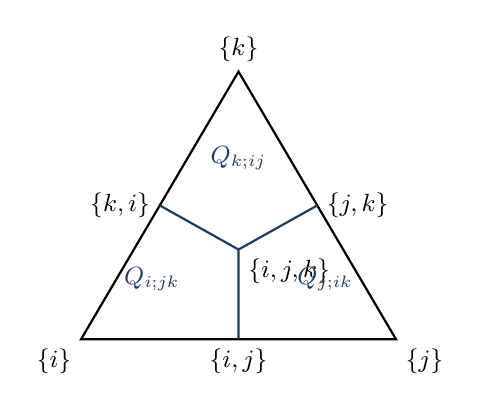
\begin{tikzpicture}[scale=2.0, every node/.style={font=\small}]
  \coordinate (A) at (0,0);
  \coordinate (B) at (2,0);
  \coordinate (C) at (1,1.7);
  \coordinate (AB) at (1,0);
  \coordinate (BC) at (1.5,.85);
  \coordinate (CA) at (.5,.85);
  \coordinate (G) at (1,.57);
  \draw[thick] (A)--(B)--(C)--cycle;
  \draw[deepblue,thick] (AB)--(G)--(CA);
  \draw[deepblue,thick] (BC)--(G);
  \node[below left] at (A) {$\{i\}$};
  \node[below right] at (B) {$\{j\}$};
  \node[above] at (C) {$\{k\}$};
  \node[below] at (AB) {$\{i,j\}$};
  \node[right] at (BC) {$\{j,k\}$};
  \node[left] at (CA) {$\{k,i\}$};
  \node[below right] at (G) {$\{i,j,k\}$};
  \node[deepblue] at (.45,.38) {$Q_{i;jk}$};
  \node[deepblue] at (1.55,.38) {$Q_{j;ik}$};
  \node[deepblue] at (1,1.15) {$Q_{k;ij}$};
\end{tikzpicture}
\caption{一つのdual triangleは3枚のmetric squareに分かれる。図は平面内の模式図であり、各青い四角形には内在的に単位Euclidean square metricを入れる。}
\label{fig:three-squares}
\end{figure}

\subsection{解釈：truncated tropical projective plane}

$\{u_i\geq0,\min u_i=0\}$ は tropical projective plane $\mathbb{TP}^2$ の標準modelである。したがって三重点のdiameter-scale geometryは、Cheng--Yau simplexのlarge-scale tropicalizationとして
\[
 \mathbb{TP}^2_{\leq1}:=\{u_i\in[0,1],\min u_i=0\}
\]
を与える、という見方ができる。各chamberにEuclidean metricが入り、compact coreは三正方形の共通頂点へcollapseする。

この記述は高次元にもそのまま拡張する。$n$-simplexでは
\[
 \{u_0,\dots,u_n\in[0,1]:\min u_i=0\}
\]
という $n+1$ 個のunit $n$-cubeの和が自然に現れる。したがって本例は、general type degenerationにおける ``cubical tropicalization'' の最初の非自明なglobal surface modelと考えられる。

\section{global候補空間 $\cC_5$}

\subsection{定義}

\begin{definition}[cubical barycentric subdivision]\label{def:C5}
$K=\Sk_2\Delta^4$ の非空faceを頂点とし、各三角形
$\sigma=\{i,j,k\}$ とその頂点 $i\in\sigma$ に対して
\begin{equation}\label{eq:squarecell}
 Q_{i;jk}
 =\bigl\{\{i\},\{i,j\},\{i,k\},\{i,j,k\}\bigr\}
\end{equation}
をunit Euclidean squareとして貼る。得られるintrinsic square complexを
\[
 \cC_5:=\square K
\]
と書き、そのlength metricを $d_{\square}$ とする。
\end{definition}

より具体的には、$e_0,\dots,e_4$ を $\RR^5$ の標準基底として
\begin{equation}\label{eq:ambientC5}
 \cC_5=\bigcup_{\substack{i,j,k\ \mathrm{distinct}\\j<k}}
 \left(e_i+[0,1]e_j+[0,1]e_k\right)\subset\RR^5
\end{equation}
と実現できる。ただしmetricはambient Euclidean distanceではなく、squareを通るintrinsic length metricである。

\begin{proposition}\label{prop:cellcount}
$\cC_5$ のセル数は
\[
 (f_0,f_1,f_2)=(25,50,30).
\]
また $|\cC_5|$ は $|K|$ とhomeomorphicであり
\[
 \chi(\cC_5)=25-50+30=5,
 \qquad
 \cC_5\simeq\bigvee^4S^2.
\]
\end{proposition}

\begin{proof}
頂点は $\{0,\dots,4\}$ のcardinality $1,2,3$ のsubsetなので
$5+10+10=25$。辺は $1$-faceから$2$-faceへのinclusionが $2\binom52=20$ 本、$2$-faceから$3$-faceへのinclusionが $3\binom53=30$ 本。squareは各三角形につき3枚なので $3\binom53=30$。各三角形を\cref{fig:three-squares}のようにcell subdivisionしているだけなのでunderlying topologyは変わらない。
\end{proof}

\subsection{strataとの対応}

$\cC_5$ の頂点labelはmetric degenerationの三種類のscaleを同時に記録する。
\[
 \begin{array}{c|c|c}
 \text{label }I&|I|&\text{幾何的意味}\\
 \hline
 \{i\}&1&H_i\text{ のcompact core}\\
 \{i,j\}&2&L_{ij}\text{ のgeneric neck core}\\
 \{i,j,k\}&3&p_{ijk}\text{ のsimplex core}
 \end{array}
\]
一つのsquare $Q_{i;jk}$ は、成分 $H_i$ の中で二本のboundary line $L_{ij},L_{ik}$ へ向かう二つのcusp depthを同時に記録する。

raw dual complexでは componentが頂点、double locusが辺、triple locusが三角形に対応する。diameter-scaleでは各stratum自身のcompact coreも新たなvertexとして可視化されるため、face posetの頂点化とcubical subdivisionが自然に現れる。

\subsection{五つのcomponent starsとfixed-pair asymptotic cones}

各$i$に対してclosed star
\begin{equation}\label{eq:Qi-star}
 Q_i=\{w\in\cC_5:w_i=1\}
\end{equation}
を置く。これは$H_i^\circ=\PP^2\setminus4L$の一つのtruncated cusp coneに対応する。

\begin{proposition}[star decomposition]\label{prop:star-decomposition}
\begin{equation}\label{eq:C5-union-stars}
 \cC_5=\bigcup_{i=0}^4Q_i.
\end{equation}
各$Q_i$は6枚のunit squaresからなり、orthant complex
\begin{equation}\label{eq:O4}
 \mathscr O_4=
 \{v\in\RR_{\ge0}^{\{0,\dots,4\}\setminus\{i\}}:
      |\supp v|\le2\}
\end{equation}
のcoordinate truncation$0\le v_j\le1$とisometricである。また
\begin{align}
 Q_i\cap Q_j
 &=\bigcup_{k\ne i,j}\{e_i+e_j+s e_k:0\le s\le1\},
 \label{eq:star-double-overlap}\\
 Q_i\cap Q_j\cap Q_k&=\{e_i+e_j+e_k\}.
 \label{eq:star-triple-overlap}
\end{align}
従ってdouble overlapは3本のunit intervalsを一点で貼ったtripod、triple overlapは一点である。
\end{proposition}

\begin{proof}
$w\in\cC_5$では$\max_iw_i=1$なので少なくとも一つの$Q_i$に属する。$Q_i$上では残る4 coordinatesのうち高々2個だけがnonzeroで、各pairが一枚のunit squareを与える。overlap formulasは$w_i=w_j=1$およびsupport boundを直接用いればよい。
\end{proof}

fixed component
\[
 U_i=H_i\setminus D_i=\PP^2\setminus4L
\]
のboundary dual complexは$K_4$ graphである。Rochon--Zhangのfacewise Poincaré expansion\cite{RochonZhang}を6個のcorner chartsで貼ると、compact coreとcircle directionsはblow-downでcollapseし、radial blocks$\sum d\rho_j^2$が\eqref{eq:O4}へ貼られる。従って$U_i$のfixed-pair KE metricのasymptotic coneは$\mathscr O_4$であり、$Q_i$はそのunit coordinate truncationである。この記述から、global candidateは「五つのcomponent asymptotic conesをtripod overlapsでglueしたもの」としても得られる。

\subsection{dominant-star reduction}

sharp actual limitを得るために、tie strataを含む全域でtensorを一様に$1+o(1)$比較する必要はない。各$Q_i$のunique-dominant open part
\begin{equation}\label{eq:Qi-open}
 Q_i^\circ=\{w\in Q_i:w_j<1\text{ for every }j\ne i\}
\end{equation}
だけでpath lengthsを同定すれば十分である。

\begin{theorem}[dominant-star patching criterion]\label{thm:dominant-star-criterion}
$(X_t,R_t^{-2}g_t)$のsubsequenceが、depth mapsを通じて$\cC_5$上の$d_\square$と双Lipschitzなcompact length metric$d_\infty$へ収束したとする。さらに、$Q_i^\circ$内に含まれる任意のLipschitz curve$\gamma$について
\begin{equation}\label{eq:open-star-length-equality}
 L_{d_\infty}(\gamma)=L_{d_\square}(\gamma)
\end{equation}
が成り立つとする。このとき$d_\infty=d_\square$である。
\end{theorem}

\begin{proof}
unique-dominant locus$\bigcup_iQ_i^\circ$は$\cC_5$でdenseであり、そのcomplementはfinite $1$-skeletonの一部である。square complex上の任意のrectifiable pathは、端点を固定したままtie edgesから隣接squareのinteriorへ任意に小さく押し出せる。このperturbationは$d_\square$-lengthを任意に小さくしか増やさない。$d_\infty$と$d_\square$は双Lipschitzなので、同じperturbationの$d_\infty$-costも一様に小さくできる。

$d_\square$のalmost-geodesicをunique-dominant locusへ押し出し、\eqref{eq:open-star-length-equality}を用いると$d_\infty\le d_\square$。逆に$d_\infty$のalmost-geodesicを同様に押し出すと$d_\square\le d_\infty$。従って両者は一致する。
\end{proof}

解析的には、\cref{thm:dominant-star-criterion}のhypothesisは次の\emph{mesoscopic component stability}へ還元される。すなわち任意の$\delta>0$に対し、非dominant depthsが$(1-\delta)R_t$以下の領域で$g_t$をfixed complete metric$g_{i,\mathrm{KE}}$とnormalized path-lengthの意味で比較する。tie layersとtriple coresはcoarse双Lipschitz controlで押し出せるので、そこでsharp tensor expansionを直接証明する必要はない。これは前版のglobal $1+o(1)$ radial estimateより明確に弱いtargetである。

\section{$\sqrt{13}$ の厳密な距離計算}

本節は元のKE問題から独立な、候補square complexの完全に厳密な計算である。

\begin{proposition}\label{prop:sqrt13}
$A=\{0,1\}$、$B=\{2,3,4\}$ を $\cC_5$ の頂点とする。このとき
\begin{equation}\label{eq:sqrt13distance}
 d_{\square}(A,B)=\sqrt{13}.
\end{equation}
\end{proposition}

\subsection{上からの評価：4枚のsquareを展開する}

次の4枚のsquareを順に通るgalleryを考える。
\begin{equation}\label{eq:gallery}
 Q_{1;02},\quad Q_{2;01},\quad Q_{2;13},\quad Q_{2;34}.
\end{equation}
これらを平面へ展開すると、順に
\[
 [0,1]\times[0,1],\quad
 [0,1]\times[1,2],\quad
 [-1,0]\times[1,2],\quad
 [-1,0]\times[2,3]
\]
という階段型polyominoになる。$A$ は $(1,0)$、$B$ は $(-1,3)$ に移る。両点を結ぶ直線は
\[
 (1-2s,3s),\qquad0\leq s\leq1
\]
であり、
\[
 s=\frac13,\frac12,\frac23
\]
でそれぞれgalleryの共有辺を横切る。したがって全直線が展開された4-square union内にあり、元のcomplexへ戻すと長さ
\begin{equation}\label{eq:upper13}
 \sqrt{(-2)^2+3^2}=\sqrt{13}
\end{equation}
のpathを得る。

元の $\RR^5$ coordinateで交点は
\[
 (1,1,0,0,0),
 \left(\frac13,1,1,0,0\right),
 \left(0,\frac12,1,0,0\right),
 \left(0,0,1,\frac13,0\right),
 (0,0,1,1,1)
\]
である。

\begin{figure}[ht]
\centering
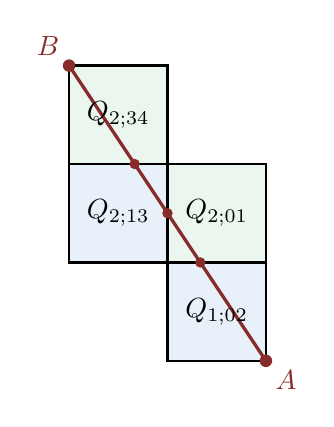
\begin{tikzpicture}[scale=1.25]
  \fill[softblue] (0,0) rectangle (1,1);
  \fill[softgreen] (0,1) rectangle (1,2);
  \fill[softblue] (-1,1) rectangle (0,2);
  \fill[softgreen] (-1,2) rectangle (0,3);
  \draw[thick] (0,0) rectangle (1,1);
  \draw[thick] (0,1) rectangle (1,2);
  \draw[thick] (-1,1) rectangle (0,2);
  \draw[thick] (-1,2) rectangle (0,3);
  \draw[deepred,very thick] (1,0)--(-1,3);
  \fill[deepred] (1,0) circle (1.8pt) node[below right] {$A$};
  \fill[deepred] (-1,3) circle (1.8pt) node[above left] {$B$};
  \fill[deepred] (1/3,1) circle (1.5pt);
  \fill[deepred] (0,1.5) circle (1.5pt);
  \fill[deepred] (-1/3,2) circle (1.5pt);
  \node at (.5,.5) {$Q_{1;02}$};
  \node at (.5,1.5) {$Q_{2;01}$};
  \node at (-.5,1.5) {$Q_{2;13}$};
  \node at (-.5,2.5) {$Q_{2;34}$};
\end{tikzpicture}
\caption{$A$ と $B$ を結ぶ長さ $\sqrt{13}$ の展開geodesic。}
\label{fig:sqrt13path}
\end{figure}

\subsection{下からの評価：piecewise linear calibration}

各squareを singleton vertexとtriple vertexを結ぶdiagonalで二つのright triangleへ分割する。$P=\{0,1\}$、$Q=\{2,3,4\}$ とし、頂点 $I$ に
\[
 a=|I\cap P|,
 \qquad b=|I\cap Q|
\]
を対応させる。次の表でpiecewise linear function $h$ の頂点値を定める。
\begin{equation}\label{eq:htable}
\begin{array}{c|cccccccc}
(a,b)&(2,0)&(1,0)&(2,1)&(1,1)&(1,2)&(0,1)&(0,2)&(0,3)\\
\hline
\sqrt{13}\,h&0&2&3&5&7&8&10&13
\end{array}
\end{equation}
各right triangleはsubset chain
\[
 I_1\subset I_2\subset I_3,
 \qquad |I_r|=r
\]
に対応する。表を直接調べると、chainに沿う二つのincrementは、符号を除けば常に $2$ と $3$ である。したがって各unit right triangle上のaffine gradientは
\[
 |\nabla h|^2=\frac{2^2+3^2}{13}=1.
\]
よって $h$ は $\cC_5$ 全体で1-Lipschitzである。一方
\[
 h(B)-h(A)=\frac{13}{\sqrt{13}}=\sqrt{13}.
\]
したがって
$d_{\square}(A,B)\geq\sqrt{13}$。上からの評価と合わせて\cref{prop:sqrt13}を得る。

\begin{remark}
このcalibrationは偶然の数値一致ではない。展開geodesicの変位vector $(-2,3)$ と、各triangle上のgradient vector $(\pm2,\pm3)/\sqrt{13}$ が双対になっている。したがって $\sqrt{13}$ はsquare complexのcell geometryから強制される自然な定数である。
\end{remark}

\subsection{diameterに関する数値実験}

各unit squareを $1/N$ meshで切り、同一square内のmesh点をEuclidean chordで結んだweighted graphを作った。これはmesh点間のintrinsic distanceに対する上からの離散近似を与える。全点対Dijkstra計算の結果は次の通りである。

\begin{table}[ht]
\centering
\begin{tabular}{rrrrr}
\toprule
$N$ & mesh頂点数 & graph辺数 & 離散diameter & $-\sqrt{13}$\\
\midrule
2  & 105  & 870    & 3.650281540 & 0.044730264\\
3  & 245  & 3180   & 3.620461364 & 0.014910088\\
4  & 445  & 8300   & 3.618033989 & 0.012482713\\
5  & 705  & 17850  & 3.615139077 & 0.009587802\\
6  & 1025 & 33810  & 3.605551275 & $<10^{-12}$\\
7  & 1405 & 58520  & 3.610019184 & 0.004467909\\
8  & 1845 & 94680  & 3.608495283 & 0.002944008\\
9  & 2345 & 145350 & 3.607139950 & 0.001588674\\
10 & 2905 & 213950 & 3.607501502 & 0.001950227\\
12 & 4205 & 420420 & 3.605551275 & $<10^{-12}$\\
\bottomrule
\end{tabular}
\caption{$\sqrt{13}=3.605551275\ldots$。$6\mid N$ のとき\cref{fig:sqrt13path}の交点 $1/3,1/2,1/3$ がmesh上に乗る。}
\label{tab:numerics}
\end{table}

最大値を与えるmesh pairは、$S_5$-symmetryを除けば常に補集合をなすsize-2 vertexとsize-3 vertexであった。この計算から得られた予想は、本版の\cref{thm:modeldiameter}で数値近似を用いずに厳密に証明される。


\section{候補square complexのdiameterの厳密決定}
\label{sec:exact-diameter}

\cref{prop:sqrt13}により $\diam(\cC_5)\geq\sqrt{13}$ はすでに厳密である。本節では上界を有限な平面展開で証明する。squareを
\[
 Q_{i;jk}=e_i+[0,1]e_j+[0,1]e_k
 \qquad(i,j,k\ \text{distinct},\ j<k)
\]
と書く。30枚のsquareのunordered pairは465個あるが、$S_5$ の作用で9軌道になる。

\subsection{monotone gallery lemma}

\begin{lemma}[monotone gallery]\label{lem:monotone-gallery}
二枚のunit squareを平面に展開し、一方から他方へ行くために横方向のunit stepが $p$ 回、縦方向のunit stepが $q$ 回必要だとする。$p$ 個の記号 $H$ と $q$ 個の記号 $V$ の任意のshuffleに対応するmonotone square galleryがcomplex内に存在すると仮定する。このとき、始点squareの任意の点と終点squareの任意の点を、いずれか一つのgallery内のstraight segmentで結べる。
\end{lemma}

\begin{proof}
両端点を結ぶsegmentは、二枚のsquareを分離する $p$ 本のvertical grid lineと $q$ 本のhorizontal grid lineを単調に横切る。それらを横切る順序は $H^pV^q$ の一つのshuffleである。そのshuffleに対応するgalleryを選べば、隣り合う二本のgrid lineを横切る間のsegmentは対応するunit square内に入る。複数のgrid lineを同時に横切る場合は、隣接するどちらの順序を選んでもよい。
\end{proof}

この補題により、geodesic equationを解く代わりに、必要なshuffle galleryが実際に存在することだけを確認すればよい。

\subsection{9軌道と非critical軌道}

$Q_0=Q_{0;12}$ とする。9軌道と以下で用いる解析的上界は次の通りである。
\begin{table}[ht]
\centering
\small
\begin{tabular}{crll}
\toprule
軌道 & size & pair representative & analytic upper bound\\
\midrule
1&30 &$Q_{0;12},Q_{0;12}$ &$\sqrt2$\\
2&30 &$Q_{0;12},Q_{1;02}$ &$\sqrt5$\\
3&60 &$Q_{0;12},Q_{0;13}$ &$\sqrt5$\\
4&60 &$Q_{0;12},Q_{1;03}$ &$2\sqrt2$\\
5&120&$Q_{0;12},Q_{3;01}$ &$\sqrt{10}$\\
6&15 &$Q_{0;12},Q_{0;34}$ &$2\sqrt2$\\
7&60 &$Q_{0;12},Q_{3;04}$ &$\sqrt{13}$\\
8&30 &$Q_{0;12},Q_{3;12}$ &$\sqrt{10}$\\
9&60 &$Q_{0;12},Q_{3;14}$ &$\sqrt{13}$\\
\bottomrule
\end{tabular}
\caption{$S_5$ の9軌道。sizeの和は465。上界はすべて明示的galleryから厳密に従う。}
\label{tab:nine-orbits}
\end{table}

軌道1は一枚のsquare、軌道2,3は二枚のsquareを一枚の $2\times1$ rectangleへ展開すればよい。軌道4の二枚はvertex $\{0,1\}$ を共有し、軌道6の二枚はvertex $\{0\}$ を共有するので、各点から共有vertexへ行くpathにより $2\sqrt2$ 以下である。

軌道5ではgallery
\[
 Q_{0;12},\quad Q_{0;13},\quad Q_{3;01}
\]
が三枚のsquareからなる $1\times3$ stripへ展開される。$x=(a,b)\in Q_{0;12}$、$y=(c,d)\in Q_{3;01}$ をlocal coordinatesで表すと、終点squareの展開座標を $(d,c-2)$ と取れるから
\[
 d(x,y)^2\leq(a-d)^2+(b-c+2)^2\leq1+9=10.
\]

軌道8では左右二つのstraight strip
\[
 \begin{split}
 &Q_{0;12},Q_{1;02},Q_{1;23},Q_{3;12},\\
 &Q_{0;12},Q_{0;23},Q_{3;02},Q_{3;12}
 \end{split}
\]
を用いる。$x=(a,b)$、$y=(c,d)$ とすれば、それぞれの展開によるpath lengthの平方は
\[
 L_+^2=(4-a-c)^2+(b-d)^2,
 \qquad
 L_-^2=(a+c+2)^2+(b-d)^2.
\]
$s=a+c\in[0,2]$ に対して
\[
 \min\{(s+2)^2,(4-s)^2\}\leq9,
 \qquad (b-d)^2\leq1
\]
なので、$\min\{L_+,L_-\}\leq\sqrt{10}$ である。従って軌道1--6および8はすべて $\sqrt{13}$ より真に小さい上界を持つ。

\subsection{critical orbit 7}

$Q_{0;12}$ 上の点を $x=(a,b)$、$Q_{3;04}$ 上の点を $y=(c,d)$ と書く。終点squareを
\[
 [-1,0]\times[-2,-1],
 \qquad y\longmapsto(-d,c-2)
\]
へ展開する。始点squareから終点squareへは一回のleft stepと二回のdown stepが必要であり、その三つのshuffleは実際に
\[
 \begin{array}{ll}
 LDD:&Q_{0;12},Q_{0;24},Q_{0;34},Q_{3;04},\\
 DLD:&Q_{0;12},Q_{0;13},Q_{0;34},Q_{3;04},\\
 DDL:&Q_{0;12},Q_{0;13},Q_{3;01},Q_{3;04}
 \end{array}
\]
として存在する。従って\cref{lem:monotone-gallery}より、任意の点対に対してこの展開中のstraight segmentを選べる。その長さは
\begin{equation}\label{eq:orbit7-global}
 d(x,y)^2\leq(a+d)^2+(b-c+2)^2\leq2^2+3^2=13.
\end{equation}
等号が可能なのは
\[
 (a,b,c,d)=(1,1,0,1)
\]
だけであり、これはvertices $\{0,1,2\}$ と $\{3,4\}$ の組である。

\subsection{critical orbit 9}

$Q_{0;12}$ 上の点を $x=(a,b)$、$Q_{3;14}$ 上の点を $y=(c,d)$ と書く。まず終点squareを右側の
\[
 [3,4]\times[-1,0],
 \qquad y\longmapsto(4-c,-d)
\]
へ展開する。三回のright stepと一回のdown stepの全shuffleは
\[
 \begin{array}{ll}
 RRRD:&Q_{0;12},Q_{1;02},Q_{1;23},Q_{3;12},Q_{3;14},\\
 RRDR:&Q_{0;12},Q_{1;02},Q_{1;23},Q_{1;34},Q_{3;14},\\
 RDRR:&Q_{0;12},Q_{1;02},Q_{1;04},Q_{1;34},Q_{3;14},\\
 DRRR:&Q_{0;12},Q_{0;14},Q_{1;04},Q_{1;34},Q_{3;14}
 \end{array}
\]
として存在する。同様に左側の
\[
 [-3,-2]\times[-1,0],
 \qquad y\longmapsto(-2-c,-d)
\]
への三回のleft stepと一回のdown stepの全shuffleも
\[
 \begin{array}{ll}
 LLLD:&Q_{0;12},Q_{0;23},Q_{3;02},Q_{3;12},Q_{3;14},\\
 LLDL:&Q_{0;12},Q_{0;23},Q_{3;02},Q_{3;04},Q_{3;14},\\
 LDLL:&Q_{0;12},Q_{0;23},Q_{0;34},Q_{3;04},Q_{3;14},\\
 DLLL:&Q_{0;12},Q_{0;14},Q_{0;34},Q_{3;04},Q_{3;14}
 \end{array}
\]
として存在する。従って左右いずれの展開でも任意の点対をstraight segmentで結べる。

$s=a+c\in[0,2]$、$u=b+d\in[0,2]$ と置くと、左右のpath lengthは
\begin{equation}\label{eq:orbit9-two-bounds}
 L_-^2=(s+2)^2+u^2,
 \qquad
 L_+^2=(4-s)^2+u^2.
\end{equation}
従って
\begin{equation}\label{eq:orbit9-global}
 d(x,y)^2
 \leq\min\{L_-^2,L_+^2\}
 \leq9+4=13.
\end{equation}
最後の不等式で等号が起こり得るのは $s=1$、$u=2$、すなわち
\[
 b=d=1,\qquad c=1-a
\]
の場合だけである。

この残るridgeには5-square gallery
\[
 Q_{0;12},Q_{1;02},Q_{1;03},Q_{1;34},Q_{3;14}
\]
を使う。その展開で
\[
 p_a=(a,1),
 \qquad q_a=(3,-1-a),
 \qquad 0\leq a\leq1
\]
となり、segment全体がstaircaseに入る。従って
\begin{equation}\label{eq:orbit9-ridge-sharp}
 d(p_a,q_a)^2
 \leq(3-a)^2+(2+a)^2
 =13-2a+2a^2.
\end{equation}
これは $0<a<1$ で $13$ より真に小さい。$a=0,1$ の二端点だけが、互いに補集合をなすsize-$2$/size-$3$ verticesである。

\begin{theorem}[候補空間のdiameter]\label{thm:modeldiameter}
\[
 \boxed{\diam(\cC_5,d_\square)=\sqrt{13}.}
\]
diameter pairは、$\{0,1,2,3,4\}$ を二分する互いに補集合のsize-$2$ vertexとsize-$3$ vertexの組に限る。
\end{theorem}

\begin{proof}
\cref{prop:sqrt13}と $S_5$ 対称性により、すべての補集合vertex pairの距離は $\sqrt{13}$ である。一方、\cref{tab:nine-orbits}の9軌道について上のgallery boundを適用すれば、任意の二点間距離は $\sqrt{13}$ 以下である。非critical軌道では上界が真に小さく、軌道7の等号条件と軌道9のridge refinement \eqref{eq:orbit9-ridge-sharp}から、等号点対は補集合vertex pairだけである。
\end{proof}

この証明は数値近似を用いない。$N=18$ mesh計算は9軌道の発見とgallery選択に有用だったが、\cref{thm:modeldiameter}の論理的入力ではない。添付したexact gallery certificateは、上に列挙したgalleryのadjacency、平面展開、および各affine endpoint formulaを整数演算で再検証する。


\section{更新された主予想}

\subsection{model theorem、coarse actual statement、sharp statement}

balanced reference modelについては\cref{prop:reference-global}が定理である。真のKE metricについてのsharp主予想は変わらない。

\begin{conjecture}[diameter-scale cubical limit]\label{conj:main}
$R_t=\log(-\log|t|^2)$ とすると
\begin{equation}\label{eq:mainconj}
 (X_t,R_t^{-2}g_t)\xrightarrow{\GH}(\mathcal C_5,d_\square).
\end{equation}
従って
\begin{equation}\label{eq:diamconj}
 \frac{\diam(X_t,g_t)}{\log(-\log|t|^2)}\longrightarrow\sqrt{13}.
\end{equation}
\end{conjecture}

diameter-one normalizationでは
\[
 (X_t,D_t^{-2}g_t)
 \xrightarrow{\GH}
 \left(\mathcal C_5,\frac1{\sqrt{13}}d_\square\right).
\]

本版で無条件に得たのは、同じstatementがbalanced model metricsに対して成立すること、actual metricsについては\cref{thm:core-exterior-transfer}の二条件へ還元されること、である。前版のように``一つのbounded Ricci-potential lemmaが閉じればcoarse theorem''とはもはや言わない。

\subsection{measure：depth push-forwardは無条件にatomic}

Pille--Schneiderのhybrid measure theorem\cite{PilleSchneider}から、probability normalizationしたKE volume formのnon-Archimedean limitは
\begin{equation}\label{eq:atomicmeasure}
 \mu_{\mathrm{NA}}=\frac15\sum_{i=0}^4\delta_{v_i}
\end{equation}
である。さらに本例では、metric convergenceを仮定せず、semistable depth mapによるpush-forwardだけなら同じatomic limitをSongのno-volume-lossから直接導ける。

$\nu_t=(10\pi^2)^{-1}\omega_t^2/2$をprobability KE volumeとし、$\Phi_t:X_t\to\cC_5$をbalanced reference constructionで用いるdepth mapとする。compact component core上では$\Phi_t\to e_i$となるようcutoffを選ぶ。

\begin{proposition}[depth-pushforward measure]\label{prop:depth-pushforward-measure}
\begin{equation}\label{eq:depth-measure-limit}
 (\Phi_t)_*\nu_t\rightharpoonup
 \frac15\sum_{i=0}^4\delta_{e_i}
\end{equation}
がweakly成り立つ。
\end{proposition}

\begin{proof}
$U_i=H_i\setminus D_i$とする。任意の$\varepsilon>0$に対し、finite-volume KE metric$g_{i,\mathrm{KE}}$のcompact truncation$K_i\Subset U_i$を
\[
 \Vol(U_i\setminus K_i,g_{i,\mathrm{KE}})<\varepsilon
\]
となるよう選ぶ。Songのmulti-pointed convergenceとno-volume-loss\cite{Song}により、$t$が十分小さいとき$K_i$の互いにdisjointなimagesを$X_t$内に取り、そのunionの外の$\nu_t$-massを$O(\varepsilon)$にできる。また各imageのmassは$1/5+o(1)$である。

$K_i$上ではcomponent coordinate$i$だけが$L_t$-scaleでdominantで、他のdepthsはboundedなので、$\Phi_t$は$e_i$へ一様収束する。従って任意のcontinuous test function$h$に対し
\[
 \int h\circ\Phi_t\,d\nu_t
 =\frac15\sum_i h(e_i)+o(1)+O(\varepsilon\|h\|_\infty).
\]
$\varepsilon\to0$として結論を得る。
\end{proof}

従ってactual metricについて$\Phi_t$がGH approximationsになることさえ証明されれば、measured GH limitは自動的に
\[
 \left(\mathcal C_5,d_\square,\frac15\sum_i\delta_{e_i}\right)
\]
となる。metric supportは2次元cubical complex全体、mass supportは5 component verticesという分離が起こる。small resolution exceptional curvesはcentral divisorial componentsではなくcanonical massを持たないが、secondary rescalingでmetric bubbleが存在しないことまでは意味しない。

\subsection{volume固定・Einstein constant固定}

$\Ric(\omega_{t,\kappa})=-\kappa\omega_{t,\kappa}$ とすると
\[
 \omega_{t,\kappa}=\kappa^{-1}\omega_t,
 \qquad
 \Vol(X_t,\omega_{t,\kappa})=\frac{10\pi^2}{\kappa^2}.
\]
従って本familyではvolume固定と$\kappa$固定は同じscale choiceである。sharp予想は
\[
 \frac{D_{t,\kappa}}{R_t}\longrightarrow\frac{\sqrt{13}}{\sqrt\kappa}
\]
となり、diameter normalization後のlimitは$\kappa$に依存しない。

\section{10 punctured necksとactual KE metricへの還元}
\label{sec:PNP}

\subsection{50 independent coresから10 coupled necksへ}

50 ODPはlocal complex geometryとしては相互にdisjointであり、各点のsecondary blow-upにはTaub--NUT modelが期待される。しかしfirst-scale neck geometryでは、同じ$L_{ij}$上の5 pointsは一つのcircle fibrationと一つのreduced equationを共有する。従って``one approximate mode per node''を最初から仮定するのは適切でない。自然なanalytic unitは
\[
 (P_{ij};q_{ij,1},\ldots,q_{ij,5})\times I
\]
である。

本版までに、このanalytic unitのうち次は無条件に閉じた。
\begin{enumerate}[label=(\alph*),leftmargin=3em]
\item balanced base charge、unit cusp flux、real scalar corner constants；
\item $z$依存operatorのcontinuous spectrumを含むweighted $L^2$ inverseと唯一のscale kernel；
\item root-$0/1$ indicial rootsに付随するfiltered defect tower（第一対数層は8-dimensional）、root-$1$ resonance audit、およびno-$r\log r$ geometric subspace。growth $O(r\log r)$だけではlogarithmic orderを有限に切れないため、必要なpolyhomogeneous orderごとにfiltrationをtruncateする；
\item complex scalar coefficientsのfactorizationと、固定order-two orientation local system；
\item collapsing circle fibersを仮定したときのflat holonomyのfirst-scale invisibility；
\item Desargues networkのuntwisted/twisted star spectraとglobal coercivity。global cycle spacesはzero modesではなくeigenvalue $2$ sectorである；
\item source-generated particular solutionのlongitudinal evennessと、base-constant sectorのexact degree jump $5$。odd homogeneous matching dataで残るのは二端のaverage degreeだけである。
\end{enumerate}
従って未解決なのは``continuous spectrumをinvertできるか''でも``global graph cyclesがcokernelを作るか''でもなく、punctured-neck側のstandard/common Laurent--Jordan transferでもleading scale residueでもない。残るのは、triple-corner側のregular filtered renormalized Calder\'on maps、regular scale-channel modulationのJacobian、odd average-degree matching、cusp-weighted Schauder/polyhomogeneous estimates、Taub--NUT source insertion、nonlinear Monge--Ampère correction、actual-family metric comparison、およびsharp metric comparisonである。

\subsection{Punctured Neck Package}

\begin{definition}[Punctured Neck Package]\label{def:PNP}
family \eqref{eq:family}が\emph{Punctured Neck Package}を満たすとは、10個のdouble strataに対し、source neighborhoods $B_{t,ij,a}$、punctured-neck regions $\mathcal N_{t,ij}$、triple-corner regions $\mathcal T_{t,ijk}$を選べて、次が成り立つことをいう。
\begin{enumerate}[label=(PN\arabic*),leftmargin=3.4em]
\item \textbf{$z$依存neck approximation。}
$\mathcal N_{t,ij}$から三つのcusp endsと五つのsource coresを除いた部分で、actual KE metricは、\cref{thm:balanced-five-source,thm:linear-five-source}のdataを持つlogarithmic Mandel modelと一様双Lipschitzであり、longitudinal parameterは$T_{ij}\asymp L_t$を満たす。
\item \textbf{polyhomogeneous cusp-to-corner matching。}
各$P_{ij}$の三つのunit-slope cusp endsは、対応する$\mathcal T_{t,ijk}$内のstandard $r=3$ toroidal modelへ$o(R_t)$ additive distortionで接続する。real scalar constantsは\cref{thm:global-scalar-matching}、complex constantsは$\mathfrak o_\Gamma$でtwistした\cref{thm:complex-cusp-factorization}と一致する。残るnormal/log modesについてlocal renormalized Calder\'on formsが\eqref{eq:local-star-coercivity}を満たし、\cref{thm:network-calderon-transfer}のglobal matchingを通過する。
\item \textbf{source-core stability。}
50 source coresのintrinsic diametersの総和は$o(R_t)$であり、core replacementは異なるboundary arms間にorder-$R_t$のshortcutを作らない。circle-fiber diametersも$o(R_t)$である。
\item \textbf{weighted filtered-defect invertibility and nonlinear correction。}
\cref{thm:mandel-factorization}のscale kernelをglobal parameterで固定し、root-$0/1$ filtered towerをapproximate solutionに必要な有限logarithmic orderでtruncateしてcorner matching variablesとして分離する。punctured-neck側のstandard/common transferは\cref{thm:standard-filtered-transfer,thm:common-filtered-transfer}で決定済みである。triple-corner側では第一対数層を\cref{prop:S3-corner-decomposition}の$4\times4$ channel matricesとして、より高い層を同じ$S_3$-isotypical decompositionのfiltered matricesとしてpolyhomogeneously構成する。leading Laurent scale residueを\cref{prop:toroidal-scale-synchronization,cor:reference-corner-scale-transport}で同期し、global common scaleを$t$で固定する。残るroot-$0$ relative shiftsとroot-$1$以上のfiltered scale tracesをprojected equationsから解き、\cref{prop:five-source-degree-jump}のfixed odd jumpとodd Wronskian conditionsを課した後、three-cusp/five-source linearized KE operatorに$t$-uniformなweighted Hölder right inverseが存在する。さらにapproximate solutionのnonlinear errorに対するcontraction estimateが成立する。
\item \textbf{overlap uniformity。}
10 necks、10 triple corners、5 component regionsのcoverとpartition of unityを、overlap multiplicityおよび全weighted constantsが$t$に依存しないように選べる。
\end{enumerate}
sharp Punctured Neck Packageとは、(PN1)--(PN2)のhorizontal/radial metric comparisonが$1+o(1)$となり、全boundary distance distortionが$o(R_t)$となる場合をいう。
\end{definition}

\begin{theorem}[punctured-neck transfer]\label{thm:PNP-transfer}
component interiorsとsource-free toroidal regionsで一様Poincaré comparisonが成り立ち、Punctured Neck Packageが成立するとする。このとき
\[
 (X_t,R_t^{-2}g_t)
\]
はGH precompactであり、任意のsubsequential limitはset $\mathcal C_5$上のcompact length metric$d_\infty$として表され、あるuniform $C\ge1$に対し
\[
 C^{-1}d_\square\le d_\infty\le Cd_\square.
\]
特にlimit topologyは$\bigvee^4S^2$、Hausdorff dimensionは2であり、50 sourcesは新しいfirst-scale branch/cellを作らない。

sharp Punctured Neck Packageとsharp exterior comparisonが成り立てば
\[
 (X_t,R_t^{-2}g_t)\xrightarrow{\GH}(\mathcal C_5,d_\square),
 \qquad
 \frac{\diam(X_t,g_t)}{R_t}\to\sqrt{13}.
\]
\end{theorem}

\begin{proof}
10 necksを、五つのsource coresと三つのcusp endsに沿って切る。(PN2)によりcusp endsは既存の$C_3$ corner chartsへ同じfirst-scale coordinatesで貼られる。(PN3)と\cref{thm:sublinear-surgery}により50 source coresをbalanced auxiliary coresで置き換えてもnormalized GH distanceは$o(1)$である。(PN1)、(PN4)、(PN5)とexterior comparisonにより、置換後のactual metricとbalanced modelは全cover上で一様双Lipschitzである。\cref{prop:reference-global,thm:core-exterior-transfer}を適用してcoarse conclusionを得る。sharp caseでは全chartのadditive distortionが$o(R_t)$なので、同じcorrespondenceがexact convergenceを与える。
\end{proof}

\subsection{secondary geometry}

first scaleでは各sourceはbalanced cornerへcollapseするが、$T_{ij}^{-1}$級のrescalingではTaub--NUT bubblesが期待される。$P_{ij}$自身はcomplex-rigidなpair of pantsなので、一つのdouble stratumに沿うcontinuous dataは主としてunordered divisor
\[
 Z_{ij}=q_{ij,1}+\cdots+q_{ij,5}
\]
に入る。従ってsecondary metricが五つのcenter positionsを回収するなら、leading cubical limitが忘れるsmoothing dataを次のscaleが記録するsecondary Torelli phenomenonになる。

ただし10 divisors $Z_{ij}$は一つのglobal quintic form $F_5$のrestrictionsであり、独立ではない。またordered small resolutionsのflop choicesは一般fiberのmetricには影響しないため、secondary invariantを定義するときもraw ODP familyからflop-invariantに構成しなければならない。

\section{証明戦略の再改訂}

\subsection{Step 1：local cusp/corner Calder\'on blocksを構成する}

weighted Hilbert/Sobolev problemは\cref{thm:mandel-factorization,thm:weighted-end-identity,prop:global-weighted-Hilbert-parametrix}で解決した。さらに\cref{thm:standard-filtered-transfer,thm:common-filtered-transfer,prop:all-regular-slope-energy}により、punctured-neck側のstandard/common towersは両parityで任意の有限logarithmic orderにおいてexactに決まり、regular Hilbert-even root-$1$ trace formはfull $\RR^3$上でcoerciveとなった。次はGuedes Bonthonneau--Lefeuvreのhyperbolic-cusp Fredholm framework\cite{GBL}またはexplicit Fourier--Mellin constructionを用い、このfiltered asymptotic moduleをweighted Hölder--Zygmund/polyhomogeneous spaces上のrenormalized Dirichlet-to-Neumann mapsへ持ち上げる。standard triple cornerでは\cref{prop:S3-corner-decomposition}により、各parityの$12\times12$ first-layer matrixは二つの$4\times4$ channel blocksへ縮約される。高いlog orderでは同じ$S_3$ decompositionを各filtered layerへ適用する。新たに計算すべき本質は、triple-corner側のfiltered standard/sign blocksとLaurent residuesのkernel/rangeである。

\subsection{Step 2：network coercivityとresonance equations}

local star coercivityが得られた後のglobal incidence inversionは\cref{thm:desargues-star-spectra,thm:network-calderon-transfer}で解決した。ordinary/twisted $H^1$ cycle spacesはzero modesではなくeigenvalue $2$ sectorである。punctured-neck側のstandard/common filtered transfersは任意の有限logarithmic orderで決定済みであり、regular even slope blockはdiagonalを含め正である。従って残るglobal finite-dimensional equationsは、triple-corner側のregular filtered standard/sign response、regular scale-channel modulationのprojected equations、odd average-degree/Wronskian matchingに限られる。leading even residueの同期とfive-sourceの相対$u_1$ jumpは\cref{prop:toroidal-scale-synchronization,prop:five-source-degree-jump}で既に固定されている。circle phase holonomyそのものはfiber collapseが得られれば\cref{lem:circle-holonomy-invisible}によりfirst-scale metricから消える。

\subsection{Step 3：actual-family parameterとTaub--NUT source insertion}

各$q_{ij,a}$の近傍にTaub--NUT approximate metricを挿入し、core regularity scaleと$T_{ij}$の関係を追う。\cref{cor:T-L-matching}が与えるmodel consistency $T_{ij}\asymp L_t$をactual familyから証明し、source-core diameter、circle-fiber diameter、boundary distortionを$o(R_t)$で評価する。さらに異なるarms間にshortcutが無いことをbarrierまたはcalibrationで示す。

\subsection{Step 4：nonlinear logarithmic Mandel neck}

balanced potential $H_Z$、linear solution \eqref{eq:linear-five-source-solution}、Taub--NUT cores、three-cusp defect coefficientsを組み合わせてapproximate negative KE metricを作る。Step 1のright inverseを用い、weighted Monge--Ampère errorをNewton iterationまたはcontraction mappingで修正する。10 necksを同時に扱い、constantsをsource positionsに一様に保つ。

\subsection{Step 5：10 triple cornersとtoroidal exterior}

$p_{ijk}$では$P_{ij},P_{ik},P_{jk}$の三つのcusp endsを一つの$r=3$ toroidal cornerへ同時に貼る。source coresとcompact neck coresの外ではRuan--Zhang proper framesをlocalizedし、moving-depth range $0\le\rho_i\le R_t+O(1)$で一様comparisonを得る。その後、五つのunique-dominant regionsでactual path lengthsをfixed complete component metricsと比較する。

\subsection{Step 6：global calibrationとgallery lift}

semistable depth map
\[
 \Phi_t:X_t\longrightarrow\mathcal C_5,
 \qquad p\longmapsto \left(\frac{\rho_i(p)}{R_t}\right)_i
\]
をcutoff付きで定義する。下側評価には$\mathcal C_5$上のpiecewise-linear calibrationsをalmost-Lipschitz functionsへliftし、上側評価には9 orbit representativesのfinite galleriesをcomponent、punctured-neck、triple-corner chartsへliftする。目標は
\begin{align}
 \sup_{p,q}\left|R_t^{-1}d_{g_t}(p,q)
 -d_\square(\Phi_t(p),\Phi_t(q))\right|&\to0,\label{eq:distortiongoal-v07}\\
 d_H(\Phi_t(X_t),\mathcal C_5)&\to0.\label{eq:densegoal-v07}
\end{align}
\cref{thm:dominant-star-criterion}により、unique-dominant starsでsharp path comparisonが閉じればtie strataのfull tensor convergenceを別に要求せずexact metricへ進める。

\subsection{Step 7：measured limitとsecondary geometry}

\cref{prop:depth-pushforward-measure}のdepth mapをhybrid retractionと同定する。first-scale measured GH theoremを閉じた後、$T_{ij}^{-1}$級rescalingから$Z_{ij}$のfive-center dataを回収する。complex period\eqref{eq:complex-secondary-period}、Taub--NUT centers、orientation local systemのうち、Riemannian metric、Kähler form、complex structureがそれぞれどの情報を保持するかを分離する。

\section{短期的に実行すべき研究項目}

\begin{enumerate}[label=\textbf{P\arabic*.},leftmargin=3.2em,itemsep=2mm]
\item \textbf{triple-corner filtered Calder\'on blocks。} standard $r=3$ cornerのtrivial/signおよびstandard representationsについて、first layerの$4\times4$ blocksを構成し、その後各logarithmic orderへfiltered extensionする。self-adjointness、flux formula、standard/sign blocksのuniform positivityを証明する。punctured-neck側の全有限次数transferとglobal 30-incidence inversionは既に閉じている。
\item \textbf{regular scale-channel corner map。} leading root-$0$ residueのparallel transportとfamily normalizationはreference/toroidal levelでは\cref{prop:toroidal-scale-synchronization,cor:reference-corner-scale-transport}で決定済みである。actual triple-corner operatorについてこのidentificationのstabilityを示し、root-$0$ relative shiftsおよびroot-$1$以上のcusp-dependent scale tracesに対するregular filtered matrixを構成する。
\item \textbf{root-$1$ scale-channel audit。} approximate Monge--Amp\`ere errorの各cuspにおける$r$ coefficient $G$を抽出し、\cref{prop:root-one-resonance-audit}のmoment $\int G\,dw$を計算する。divergence structureにより消える場合を同定し、一般の場合はtriple-corner filtered scale traceとともにprojected modulation equationとして解く。
\item \textbf{weighted Hölder--polyhomogeneous upgrade。} \cref{prop:global-weighted-Hilbert-parametrix}をhyperbolic-cusp calculusまたはexplicit Fourier--Mellin analysisへ持ち上げ、filtered trace blockを付加した$t$-uniform right inverseを構成する。
\item \textbf{low-energy modulation audit。} $u_0=\partial_{\log T}$のdictionaryを用い、root-$0$ relative shifts、root-$1$以上のcusp-dependent scale traces、projected nonlinear errorのJacobianを計算する。global common leading shiftは$t$が固定し、全scale-channel correctionが$o(R_t)$なら\cref{prop:scale-modulation-invisible}の議論によりfirst-scale metricから消える。
\item \textbf{Mandel parameter matching。} fixed cutoffに依存する$O(1)$を追跡し、actual familyから$T_{ij}/L_t$のuniform upper/lower bounds、可能なら$T_{ij}=c_{ij}L_t(1+o(1))$を導く。
\item \textbf{Taub--NUT core estimate。} 各source coreとcircle fibersのdiameter、boundary shortcutを$o(R_t)$で評価する。50個を独立にではなく、各balanced five-source neckのweighted normの中で同時に制御する。
\item \textbf{nonlinear punctured neck。} $H_Z$と\eqref{eq:linear-five-source-solution}をbackground dataとしてapproximate negative KE metricを構成し、weighted Monge--Ampère correctionを閉じる。
\item \textbf{triple-corner diagonal channels。} orientation-twisted complex constants、even regular scale-channel coefficients、odd average-degree/Wronskian dataを一つの$r=3$ cornerへ同時にmatchする。leading diagonal scale lineは\cref{cor:reference-corner-scale-transport}で既知なので、actual operatorのkernelがその幾何学的mode以外を持たないことを示す。
\item \textbf{toroidal exterior localization。} component interiorsとsource-free collarsでRuan--Zhang estimatesをlocalizedし、Punctured Neck Packageの外側hypothesisを閉じる。
\item \textbf{dominant-star and calibration transfer。} unique-dominant regionsでactual path lengthsを比較し、$\sqrt{13}$ lower calibrationと9-orbit upper galleriesを10-neck coverへliftする。
\item \textbf{secondary period hierarchy。} $\mathcal P_{\mathrm{bal}}\in\RR^9$、$\mathcal P_{\CC}\in(\CC^\times)^9$、fixed orientation local system、Taub--NUT center dataをmultiscale invariantとして統一する。
\end{enumerate}

\section{どこまでが定理で、どこからが未完か}

\begin{longtable}{p{0.25\textwidth}p{0.65\textwidth}}
\toprule
区分 & 内容\\
\midrule
\endfirsthead
\toprule
区分 & 内容\\
\midrule
\endhead
既存定理 & fixed Einstein scaleのmulti-pointed limit/no-volume-loss、Ruan--Zhangのoriginal ample/$\mathbf Q$-factorial hypotheses下のuniform comparison、toroidal pointed collapse、hybrid KE measure、Mandelのcompact-base abstract neck constructionとそのpointed multiscale limits。\\[1mm]
厳密代数幾何 & $\mathcal T^1|_{L_{ij}}=\mathcal O(5)$、50 ODP、ordered projective small crepant semistable resolutions、global $d$-semistability、Euler数55、120 ordered modelsの$A_4$ braid chambersと5-curve adjacent flops。\\[1mm]
static punctured-neck theory & balanced five-source potential、各cuspの展開$r+2\log r+\beta_c+O(e^{-r})$、unit fluxとexact $5=2+3$、absolute cusp-period formula、balanced real scalar classのvanishing、$\mathcal P_{\mathrm{bal}}(F_5)\in\RR^9$。\\[1mm]
本版のlinear analytic theorem & exact Pöschl--Teller factorization、one-dimensional weighted $L^2$ kernel、kernel complementのuniform spectral gap、continuous spectrumを含むnormalized Fredholm inverse、Green multiplierのorder $-1$ estimate、linear five-source distributional solution。\\[1mm]
本版のcusp/phase theorem & first logarithmic layerの8 modes、全filtered defect tower $\dim\mathfrak D_N=4(N+1)$、root-free indicial strips、central-strip weighted Hilbert Fredholm theorem、root-$1$ resonance audit、complex cusp factorization、非自明なorder-two orientation local system、$\mathcal P_{\CC}(F_5)\in(\CC^\times)^9$、sublinear circle fibersに対するholonomy invisibility。\\[1mm]
本版の$\Gamma(2)$ scattering theorem & cusp width $2$のgeometric normalization、trivial/standard scattering eigenvalues、standard channelの全有限log-order非退化、common channelのall-order Laurent--Jordan transfer modulo residue、$D_{\mathrm{triv}}$の明示式、first common Jordan formula、full regular Hilbert-even root-$1$ trace formのasymptotic coercivity。\\[1mm]
本版のCalder\'on network theorem & untwisted/twisted star operatorsのexact spectra、gaps $1/3$と$1-\sqrt5/3$、cycle spacesがeigenvalue $2$ sectorであること、local star positivityからglobal coercivityへのtransfer、$S_3$によるcorner $12\times12$ matrixの二つの$4\times4$ blocksへの縮約、five-source forcingのeven parity。\\[1mm]
v0.12 scale--degree／toroidal theorem & $u_0=\partial_{\log T}$と$u_1=\partial_\alpha$のexact Jacobi-field dictionary、five-source coefficient jump $5$、全30 incidencesの$\log\Lambda=R_t+O(1)$、source-free reference cornerのdiagonal scale transport、sublinear overlap-compatible modulationのfirst-scale invisibility。\\[1mm]
厳密有限幾何 & $\mathcal C_5$のcell structure/位相、465 square pairsの9軌道分類、$\diam(\mathcal C_5)=\sqrt{13}$、diameter pair分類。\\[1mm]
model metric theorem & balanced auxiliary familyのglobal cubical limitとdiameter asymptotics、five-star decomposition、dominant-star patching criterion、finite sublinear surgery invariance。\\[1mm]
条件付きactual theorem & 更新されたPunctured Neck Packageとtoroidal exterior comparisonから、actual subsequential limitsが$\mathcal C_5$上で$d_\square$と双Lipschitzであること。sharp packageならexact $d_\square$と$D_t/R_t\to\sqrt{13}$。\\[1mm]
actual theoremの未完部分 & continuous $L^2$ spectrum、complex scalar class、punctured-neck standard/common filtered transfers、regular common slope、global Desargues network inversion、leading toroidal scale synchronization、five-source degree jumpは解決済み。未完なのはweighted Hölder--Zygmund/polyhomogeneous upgrade、triple-corner regular filtered blocks、regular scale-channel modulation Jacobian、odd average-degree matching、nonlinear neck、actual-family $T_{ij}=L_t\,e^{O(1)}$ and metric comparison、Taub--NUT core/fiber no-shortcut、sharp exterior and dominant-star stability。\\[1mm]
measure & actual KE volumeのdepth push-forwardは$\frac15\sum_i\delta_{e_i}$へ収束する。measured GH theoremには同じdepth mapがmetric GH approximationになることの証明が残る。\\[1mm]
撤回・修正した見通し & fixed vertical polarizationからstandard $C^2$ estimatesが直ちに得られるというv0.3の見通し、50 nodesを50 independent analytic modesとして扱うv0.4の作業仮説、およびcontinuous spectrum自体が主要Fredholm obstructionであるというv0.6の見通し。\\
\bottomrule
\end{longtable}

\section{展望}

本版で最も重要な進展は、Mandelの二つのlongitudinal zero modesをscaleとdegreeのJacobi fieldsとして同定し、五点源がdegree coefficientにexact jump $5$を与えること、さらに$xyz=t\vartheta$のtoroidal normal formから全30 incidencesのleading logarithmic scaleを同期したことである。これによりglobal even scale lineはreference/toroidal levelで$t$により固定され、root-$1$ momentはcusp-dependent correctionを含むscale-channel modulation equationとして扱うべきことが分かった。v0.11で得たfiltered tower、all-order $\Gamma(2)$ transfer、Pöschl--Teller coercivity、Desargues network gapsはそのまま維持される。従って主予想を阻んでいるのは一般的なspectral pathologyでもpunctured-neck側のJordan renormalizationでもglobal graph cohomologyでもleading scale residueでもなく、triple-corner側のregular filtered Calder\'on blocks、regular scale-channel modulationのJacobian、odd average-degree matching、Taub--NUT cores、nonlinear resonant errorである。

complex phaseについても構図が変わった。actual smoothing sectionのphasesはarbitraryな$H^1(\Gamma;S^1)$ classを作らず、固定されたorder-two orientation local systemとglobal triple-point valuesへfactorする。前者はcircle fibersがcollapseすればfirst-scale GH metricから消え、後者はcomplex secondary periodとして残る。したがってfirst-scale metric theoremとsecondary holomorphic dataを論理的に分離できる。

今後の論文構成は次の三段階が自然である。
\begin{enumerate}[label=(\roman*),leftmargin=3em]
\item \textbf{exact algebraic/linear/cubical paper。}
対数的charge identity、ordered semistable models、balanced potential、Pöschl--Teller factorization、complex orientation local system、balanced cubical model、$\sqrt{13}$ theorem、Punctured Neck Packageへの還元をまとめる。本稿の無条件部分は既に独立した論文核を持つ。
\item \textbf{logarithmic Mandel gluing theorem。}
filtered defect tower（第一対数層は8-dimensional）とcentral-strip Fredholm estimateを持つthree-cusped pair of pants上のfive-source negative KE neckを構成し、三つのcusp endsをtriple cornersへglueする。これがactual coarse GH theoremの本丸である。
\item \textbf{sharp and secondary geometry。}
$1+o(1)$ radial comparison、dominant-star criterion、calibration/gallery liftからexact $d_\square$と$\sqrt{13}$を得る。その後、$\mathcal P_{\CC}$とTaub--NUT rescalingから$Z_{ij}$の残余five-point dataを回収する。
\end{enumerate}

quintic caseが特に魅力的なのは
\[
 N_{L/H}=K_L(T)=\mathcal O(1)
\]
というself-matchingに加え、linearized neck operatorがexplicitly factorableであり、global complex signsも一つのcanonical orientation local systemへ収束することである。一般の$d$平面退化にもcharge balanceはあるが、この三つの整合性が同時に成立する本例は、general typeのdiameter-scale tropicalizationを解析する最初のglobal two-dimensional test caseとして際立っている。

現時点の最も正確な一行要約は
\[
 \boxed{\begin{gathered}
 \text{candidate cubical space、そのdiameter、static charge、linear $L^2$ theory、}\\
 \text{$\Gamma(2)$ standard scattering、regular common slope、global networkは解決した。}\\
 \text{actual KE limitはtriple-corner regular filtered blocks、scale-channel modulation、}\\
 \text{Taub--NUT cores、nonlinear resonance、sharp metric transferへ還元された。}
 \end{gathered}}
\]
である。主予想そのものはまだ証明されていないが、残る問題は以前よりはるかに局所的かつ構造化された形になった。

\appendix

\section{scale--degree／plumbing synchronization certificateの仕様}

添付した\texttt{scale\_degree\_plumbing\_certificate.py}は、\cref{prop:scale-degree-dictionary,prop:five-source-degree-jump,prop:toroidal-scale-synchronization,cor:reference-corner-scale-transport}で用いる有限・symbolic部分を検査する。具体的には次を確認する。
\begin{enumerate}[leftmargin=2.5em]
\item exact reduced family\eqref{eq:exact-mandel-two-parameter-family}が\eqref{eq:exact-mandel-reduced-ode}を満たすこと。
\item $H_0u_0=H_0u_1=0$と、\eqref{eq:u0-scale-derivative},\eqref{eq:u1-degree-derivative}のscale/degree derivative identities。
\item $m_0=\pi\operatorname{sgn}(w)u_1$、$m_0'(0+)-m_0'(0-)=2\pi$、five-source $u_1$ coefficient jumpが$5$であること、およびbalanced particular solutionの平均coefficientが$0$であること。
\item bounded unitを含むtoroidal effective scale $\Lambda=e^R(1-p)+O(1)$について、$\log\Lambda/R\to1$かつ$\partial_R\log\Lambda\to1$であること。
\item 10 necks、10 corners、30 incidencesと両側のvalency $3$。
\end{enumerate}
これはtriple-cornerのactual KE Calder\'on map、nonlinear scale-modulation Jacobian、Taub--NUT no-shortcut estimate、GH収束をcomputer proofへ置き換えるものではない。

\section{filtered scattering tower certificateの仕様}
付属スクリプト
\texttt{filtered\_scattering\_tower\_certificate.py}
は次を検査する。
\begin{enumerate}[leftmargin=2.5em]
\item $\mathsf T_{0,2}^{(p)}$, $\mathsf T_{1,2}^{(p)}$が
$H_0u_p=0$, $H_0v_p=u_p$, $H_0z_p=v_p-u_p$のformal relationsの下でexact cusp operatorにより消えること。
\item standard Taylor seriesとroot-$0/1$ towersのformal multiplicationから、\eqref{eq:standard-filtered-transfer-formula}とtruncated determinantsをorder $N\le6$まで再現すること。
\item trivial Laurent seriesから\eqref{eq:common-all-order-laurent}とquotient determinantsをorder $N\le6$まで再現すること。
\item $D_{\mathrm{triv}}$のformula \eqref{eq:Dtriv-formula}を80桁精度でdirect Laurent limitと照合すること。
\item $n=0,1$のcommon relationsが\eqref{eq:renormalized-common-cusp-expansion}, \eqref{eq:first-common-jordan-tower}を再現すること。
\end{enumerate}
このcertificateはtriple-corner Calder\'on mapやactual KE metricを検査するものではなく、punctured-neck scatteringのfiltered formal algebraを監査する。

\section{$\Gamma(2)$ scattering／Jordan certificateの仕様}

添付した\texttt{gamma2\_scattering\_jordan\_certificate.py}は、\cref{thm:gamma2-scattering-channels,thm:even-standard-jordan-block,cor:odd-standard-jordan-block,thm:renormalized-common-channel,prop:all-regular-slope-energy}のspecial-function／finite-dimensional部分を高精度で検査する。具体的には次を確認する。
\begin{enumerate}[leftmargin=2.5em]
\item cusp width $2$、$q=e^{\pi iz}$、$r=\pi\operatorname{Im}z$からoutgoing multiplier $2^s\pi^{2s-1}$が生じること。
\item Posingiesのdiagonal/off-diagonal coefficientsから$\psi_{\mathrm{std}},\psi_{\mathrm{triv}}$を再構成すること。
\item $\psi_{\mathrm{std}}(1)=-4\log2$、二通りの$\psi_{\mathrm{std}}'(1)$ formula、standard functional equationを数値高精度で照合すること。
\item trivial channelのresidue $3$とfinite part $C_{\mathrm{triv}}$を照合し、renormalized common expansionのcoefficients $(-3,C_{\mathrm{triv}})$を記録すること。
\item parity-independent standard Jordan matrixのdeterminantとsingular valuesを検査すること。
\item regular slope energyのleading coefficient $\pi^2$およびcommon logarithmic correction $-6\pi^2\|P_{\mathrm{triv}}\mathbf a\|^2\log R$を検査すること。
\end{enumerate}
scriptはEisenstein seriesのanalytic continuationそのものを証明するものではなく、文献のscattering formulasから本稿のcusp normalization、Laurent/Jordan coefficients、energy constantsへの換算ミスを排除するcertificateである。

\section{Calder\'on network coercivity certificateの仕様}

添付した\texttt{calderon\_network\_coercivity\_certificate.py}は、\cref{thm:desargues-star-spectra,rem:H1-is-maximal-energy}のfinite exact linear algebraを検査する。具体的には次を確認する。
\begin{enumerate}[leftmargin=2.5em]
\item 10 neck vertices、10 corner vertices、30 incidencesを生成すること。
\item unsigned edge--triangle inclusion block $B$について
\[
 \det(xI-B^{\mathsf T}B)=(x-9)(x-4)^4(x-1)^5
\]
であること。
\item orientation-signed block $C$について
\[
 \det(xI-C^{\mathsf T}C)=x^4(x-5)^6,
 \qquad \operatorname{rank}C=6
\]
であること。
\item これらから$Q_+$と$Q_-$のeigenvalue multiplicitiesが\eqref{eq:Qplus-spectrum}, \eqref{eq:Qminus-spectrum}と一致すること。
\item untwisted kernelがglobal constantの1次元だけであり、twisted kernelが0であること。
\end{enumerate}
scriptはlocal Calder\'on formsのanalytic constructionやpositivityを証明するものではない。それらを仮定した後のglobal network spectrum、符号、multiplicityの転記誤りを排除するcertificateである。

\section{punctured Mandel factorization certificateの仕様}

添付した\texttt{punctured\_mandel\_factorization\_certificate.py}は、\cref{thm:mandel-factorization,prop:green-multiplier,thm:linear-five-source}の有限・symbolic部分を検査する。corrected defect/indicial計算は次節の専用certificateへ分離する。具体的には次を確認する。
\begin{enumerate}[leftmargin=2.5em]
\item $w=\sinh s$、$f=(\cosh s)^{-5/2}y$によるPöschl--Teller conjugation identity。
\item $A=Q^*Q$のpotential identity。
\item $H_0u_0=H_0u_1=0$、Wronskian $W=(1+w^2)^{-3}$。
\item explicit formulas \eqref{eq:jordan-v0},\eqref{eq:jordan-v1}に対する$H_0v_i=u_i$。
\item $m_0$の左右derivative jumpが$2\pi$であること、および$T m(Tz)$のscaling identity。
\item いくつかの$\lambda>2$について、decaying numerical Green solutionが\eqref{eq:green-high-frequency-bound}を満たすこと。
\end{enumerate}
最後の項はsanity checkであり、\eqref{eq:green-high-frequency-bound}の証明は本文のenergy argumentである。このscriptはspectral theorem、Sobolev multiplier theorem、weighted cusp parametrixをcomputer proofへ置き換えるものではない。

\section{cusp indicial／weighted parametrix certificateの仕様}

添付した\texttt{cusp\_indicial\_parametrix\_certificate.py}は、\cref{prop:cusp-defect-block,thm:indicial-spectrum,thm:weighted-end-identity,prop:root-one-resonance-audit}の有限・symbolic部分を検査する。具体的には次を確認する。
\begin{enumerate}[leftmargin=2.5em]
\item $H_0u_i=0$、$H_0v_i=u_i$と、\eqref{eq:full-eight-defect-basis}の8 functionsがexact cusp operatorのkernelに入ること。
\item $h_2=w(1+w^2)^{-2}$が$H_0h_2=-2h_2$を満たすこと。
\item $\mu=0,2,9/4$から生じるindicial rootsとcontinuous threshold $(1\pm\sqrt{10})/2$。
\item central-strip energy identityのzeroth-order coefficientが$1/4-\delta^2$であること。
\item $\|u_0\|_q^2=\pi/2$、$qu_0=1$からroot-$1$ residue coefficientが$(2/\pi)\int G\,dw$となること。
\end{enumerate}
これはglobal elliptic regularityやnonlinear gluingをcomputer proofへ置き換えるものではなく、indicial signs、Jordan modes、normalization constantsの転記誤りを排除する。

\section{ordinary／twisted defect cohomology certificateの仕様}

添付した\texttt{defect\_cohomology\_certificate.py}は、\cref{prop:twisted-defect-cohomology}の有限線形代数をexactに検査する。Desargues incidence graphのordinary coboundary matrixとorientation local systemでtwistしたcoboundary matrixを構成し、
\[
 \operatorname{rank}d_{\mathrm{ord}}=19,
 \qquad
 \operatorname{rank}d_{\mathrm{tw}}=20,
\]
従って
\[
 (\dim H^0,\dim H^1)_{\mathrm{ord}}=(1,11),
 \qquad
 (\dim H^0,\dim H^1)_{\mathrm{tw}}=(0,10)
\]
であることを確認する。これはtriple-corner Calder\'on mapのrankを計算するものではなく、そのdomain/targetが入るambient coefficient systemsを検査するcertificateである。

\section{complex phase orientation certificateの仕様}

添付した\texttt{complex\_phase\_orientation\_certificate.py}は、\cref{prop:orientation-class}の有限組合せ部分を$\ZZ/2$ linear algebraで検査する。具体的には次を行う。
\begin{enumerate}[leftmargin=2.5em]
\item Desargues incidence graphの20 vertices、30 edges、$b_1=11$を再構成する。
\item ordered-triple sign cochain$\varepsilon$について、vertex coboundary matrixのrankが$19$、$\varepsilon$を加えたaugmented rankが$20$であることを確認し、$[\varepsilon]\ne0$を証明する。
\item graphのsimple $6$-cyclesを全列挙し、個数が20で、すべてのholonomyが$-1$であることを確認する。
\item 本文のexplicit cycleのholonomyと、classのorderが2であることを出力する。
\item 全$5!=120$個のlabel permutationsについて、pull-backされたsign cochainと元のcochainとの差がedge/triple orientation signsのvertex coboundaryであることを確認する。
\end{enumerate}
これはcomplex cusp coefficientのanalytic definitionを置き換えないが、30 incidencesにわたるsign bookkeepingとgraph cohomology calculationをexactに保証する。

\section{balanced potential／global scalar matching certificateの仕様}

添付した\texttt{balanced\_punctured\_neck\_certificate.py}は、\cref{thm:balanced-five-source,cor:analytic-charge,cor:absolute-cusp-period,prop:desargues-obstruction,thm:global-scalar-matching}の有限・symbolic部分を検査する。具体的には次を確認する。
\begin{enumerate}[leftmargin=2.5em]
\item pair of pantsのarea $2\pi$、charge identity $5-2-3=0$、cusp model $h_0(r)=r+2\log r$に対する$\Delta h_0=-2$とunit flux $2\pi$。
\item $S_3$-invariant reference polynomial
$(z^2-z+1)(z+1)(z-\tfrac12)(z-2)$の$z\mapsto1-z$、$z\mapsto1/z$に関するinvarianceと、$|p_*(0)|=|p_*(1)|=1$。
\item 2-subsets/3-subsets incidence graphが20 vertices、30 edges、rank $19$、$b_1=11$であること。
\item standard arrangement
$L_0=e_0^*,\ldots,L_3=e_3^*$、$L_4=-(e_0^*+\cdots+e_3^*)$に対し、minor formulaで構成した$w_{ij;k}$が全10 double linesで
$\sum_{k\notin\{i,j\}}w_{ij;k}=0$を満たすこと。
\item 同じtriple pointの三つのincidence representativesがsignを除いて一致すること。これはabsolute valuesに対するglobal scalar factorizationのfinite exterior-algebra coreを検査する。
\item triple vertices上のJohnson graph $J(5,3)$がconnectedであり、edge differencesがzero-sum normalized triple-value vectorを回収すること。
\end{enumerate}
これはGreen-current existenceやnonlinear KE gluingをcomputer proofへ置き換えるものではなく、normalization、flux、graph rank、exterior-algebra signsの転記誤りを排除するcertificateである。

\section{punctured-neck charge certificateの仕様}

添付した\texttt{punctured\_neck\_charge\_certificate.py}は、\cref{prop:log-charge,prop:degree-d-charge,prop:ten-neck-incidence,cor:T-L-matching,lem:polynomial-invisibility}の有限・symbolic部分を検査する。具体的には次を確認する。
\begin{enumerate}[leftmargin=2.5em]
\item quintic caseでnormal degrees $(1,1)$、triple divisor degree $3$、smoothing zero degree $5$が
$1+1+3-5=0$を満たすこと。
\item 一般degree $d$で$1+1+(d-2)-d=0$、かつ$\deg K_L(T)=d-4$がnormal degree $1$と一致するのは$d=5$だけであること。
\item 10 double lines、各3 cusp ends、各5 sources、10 triple points、各tripleに3 incidencesというcounts。
\item $T=L$と置いたmodel normalizationで
$\operatorname{arcsinh}L-\log L\to\log2$であり、$\operatorname{arcsinh}T=R+O(1)$が$T\asymp e^R=L$に対応すること。
\item polynomial scale $|s|=L^{-A}$に対し
$\log(L+2A\log L)-\log L\to0$であること。
\end{enumerate}
これはpunctured-neck PDEやactual metric comparisonを証明するものではなく、line-bundle degrees、incidence、scale asymptoticsの転記誤りを排除するcertificateである。

\section{ordered chamber certificateの仕様}

添付した\texttt{ordered\_resolution\_chamber\_certificate.py}は、\cref{prop:A4chambers,cor:adjacent-flop-five}の有限組合せ部分をexact integer arithmeticで検査する。120 permutationsから120 transitive orientations of $K_5$を生成し、各orderで50 exceptional curvesのpositive degree conditions、component blow-up counts、adjacent transpositionがちょうど一つのedge orientationとその上の5 curvesだけを反転すること、chamber adjacency graphが240 edgesを持つことを確認する。

\section{node weight identity certificateの仕様}

添付した\texttt{node\_weight\_identity\_certificate.py}は、fixed vertical twistのneck-end oscillation、balanced choice $\eps_t=L_t^{-1}$の$O(1)$ weight、node determinant identity
\[
 \frac{a^{-2}+b^{-2}}{(a+b)^2/(a^2b^2)}
 =\frac{a^2+b^2}{(a+b)^2}\in[1/2,1]
\]
をsymbolicに検査し、machine-readable JSONへ出力する。これはglobal PDE estimateを置き換えないが、本稿で用いるlocal algebraic identitiesの符号・factorの転記誤りを排除する。

\section{vertical twist trade-off certificateの仕様}

添付した\texttt{vertical\_twist\_tradeoff\_certificate.py}は、\cref{prop:fixed-twist-obstruction}のline-bundle/endpoint bookkeepingとbalanced scaleの指数をexact arithmeticで検査する。具体的には次を確認する。
\begin{enumerate}[leftmargin=2.5em]
\item local divisorsについて
\[
 \deg\mathcal O(D_u)|_E=1,\qquad
 \deg\mathcal O(D_x)|_E=-1,
\]
従って$\mathcal A=\mathcal O(aD_x+bD_u)$なら$d=\deg(\mathcal A|_E)=b-a$。
\item neck ends $p_t=(c,t/c,0)$、$q_t=(t/c,c,0)$ における
$\log|x^au^b|^2$の$L_t$ coefficientのabsolute valueが$|b-a|$であること。
\item 120 total ordersのすべてが50 nodesをorientし、order coordinatesでblow-up profile $(20,15,10,5,0)$を与えること。
\item fixed $N$ではleading oscillation coefficientが$d/N$で残り、balanced choice$\eps_t=L_t^{-1}$ではweight oscillationが$O(1)$、model exceptional lengthが$L_t^{-1/2}$、curvature scaleが$L_t$となること。
\end{enumerate}
このscriptはsmooth-metric determinantのanalytic estimateを証明するものではない。その部分は\cref{prop:fixed-twist-obstruction}のlocal frame calculationに属する。

\section{semistable resolution certificateの仕様}

添付した \texttt{semistable\_resolution\_certificate.py} は、\cref{prop:T1O5,thm:global-small-resolution,prop:dsemistable-resolved,prop:resolved-logcanonical} の有限組合せ部分をexact integer arithmeticで検査する。具体的には次を出力する。
\begin{enumerate}[leftmargin=2.5em]
\item 10 double lines、各5 nodes、総数50。
\item 全順序 $0<1<2<3<4$ によるcomponent blow-up counts $(20,15,10,5,0)$。
\item 各double lineで、5 nodesをどちら側へ割り当てても
\[
 (1-a)+(1-(5-a))+3=0
\]
となる$d$-semistability degree certificate。
\item component Euler numbers $(23,18,13,8,3)$ と
\[
 \sum_i e(\widetilde H_i)-10e(\PP^1)+10=55.
\]
\item 各componentで $(K_{\widetilde H_i}+\widetilde D_i)^2=1$、総canonical volume 5。
\end{enumerate}
scriptはlocal blow-upのscheme-theoretic proofを置き換えないが、50 choicesに関するdegree/Euler bookkeepingの転記誤りを排除する。

\section{厳密gallery certificateの仕様}

添付した \texttt{cubical\_diameter\_exact\_gallery\_certificate.py} は、浮動小数点演算を用いず、整数行列とsubset labelsだけで\cref{thm:modeldiameter}の有限幾何部分を再検証する。具体的には次を行う。
\begin{enumerate}[leftmargin=2.5em]
\item 30枚のsquareと465個のunordered pairを生成し、$S_5$ の120置換により9軌道とorbit sizes
\[
 30,30,60,60,120,15,60,30,60
\]
を再計算する。
\item 本文で用いたすべてのgalleryについて、隣接squareがfull edgeを共有することを確認する。
\item 各共有edgeで次のsquareを反射して平面展開し、終点squareのaffine mapが本文の整数行列・整数translationと一致することを確認する。
\item 軌道5,7,8,9のlength formulaと、軌道9のridge shortening
\[
 13-2a+2a^2=13-2a(1-a)
\]
をmachine-readable JSONへ出力する。
\end{enumerate}
このscriptは証明の概念的部分であるmonotone gallery lemmaと初等不等式を置き換えるものではないが、長いgallery listに転記誤りがないことをexact arithmeticで保証する。

\section{数値的整合性検査の定義}

$N$-meshでは、各square $Q_{i;jk}=e_i+[0,1]e_j+[0,1]e_k$ に
\[
 e_i+\frac aN e_j+\frac bN e_k,
 \qquad 0\leq a,b\leq N
\]
を置く。異なるsquareで同じambient coordinateを持つ点は同一視する。同一square内の任意の二mesh点を、そのEuclidean distanceをweightとして結ぶ。このcomplete-in-cell graphのpathはすべて $\cC_5$ 内の実際のpiecewise linear pathなので、graph distanceは対応するmesh点のintrinsic distanceの上界である。

全点対shortest pathをSciPyのsparse Dijkstraで計算した。$N=12$ では4205頂点、420420無向辺である。再現用scriptを本ノートとともに添付する。


\section{$S_5$ mesh-orbit検査の仕様}

添付scriptは次を実行する。
\begin{enumerate}[leftmargin=2.5em]
\item 30枚のsquareを生成し、$S_5$ の120置換を全探索してunordered pairのcanonical representativeを求める。
\item 各squareの $(N+1)^2$ mesh点をambient $\RR^5$ coordinateで同一視する。
\item 同一square内の全点対をEuclidean chordで結び、source squareの全mesh点からsparse Dijkstraを実行する。
\item 各orbit representativeについて $M_N$、covering upper bound、$\sqrt{13}$ certificateで未処理となるmesh pair数をCSVへ出力する。
\end{enumerate}
$N=18$ の実行では約0.6GBのmemoryを用いる。通常の再現にはdefaultの $N=12$ で十分である。これは\cref{thm:modeldiameter}とは独立な数値的整合性検査であり、9軌道の発見およびcritical galleryの探索過程を再現する。


\section{normalizationの換算}

Kähler formを $\omega'=c\omega$ とすると、Riemannian distanceは $\sqrt c$ 倍、real 4-dimensional volumeは $c^2$ 倍される。一方Ricci formはconstant rescalingで変わらないので
\[
 \Ric(\omega')=\Ric(\omega)=-\omega=-c^{-1}\omega'.
\]
したがってEinstein constant $-1$ から $-\kappa$ へ移るには $c=\kappa^{-1}$ とすればよい。

直径を1に正規化すると
\[
 \widehat g_t=D_t^{-2}g_t,
 \qquad
 \Vol(X_t,\widehat g_t)=10\pi^2D_t^{-4}\to0.
\]
また
\[
 \Ric(\widehat g_t)=-D_t^2\widehat g_t
\]
なので、diameter-one familyには一様なRicci下界がない。したがって通常のGromov compactness theoremを直接使えないことが、問題の解析的難しさの一因である。

\begin{thebibliography}{99}

\bibitem{BermanGuenancia}
R.~J. Berman and H.~Guenancia,
\emph{Kähler--Einstein metrics on stable varieties and log canonical pairs},
Geom. Funct. Anal. \textbf{24} (2014), 1683--1730; arXiv:1304.2087.


\bibitem{DoiYotsutani}
M.~Doi and N.~Yotsutani,
\emph{Differential geometric global smoothings of simple normal crossing complex surfaces with trivial canonical bundle},
Complex Manifolds \textbf{10} (2023), 20220143; arXiv:2203.09304.

\bibitem{Fox}
D.~J. F. Fox,
\emph{A Schwarz lemma for Kähler affine metrics and the canonical potential of a proper convex cone},
Ann. Mat. Pura Appl. \textbf{194} (2015), 1--42; arXiv:1206.3176.

\bibitem{FuHeinJiang}
X.~Fu, H.-J.~Hein and X.~Jiang,
\emph{A continuous cusp closing process for negative Kähler--Einstein metrics},
Geom. Funct. Anal. \textbf{35} (2025), 542--632; arXiv:2401.11468.

\bibitem{GBL}
Y.~Guedes Bonthonneau and T.~Lefeuvre,
\emph{Local rigidity of manifolds with hyperbolic cusps I. Linear theory and microlocal tools},
Ann. Inst. Fourier (Grenoble) \textbf{73} (2023), no.~1, 335--421.

\bibitem{MazzeoMelrose}
R.~Mazzeo and R.~B.~Melrose,
\emph{Pseudodifferential operators on manifolds with fibred boundaries},
Asian J. Math. \textbf{2} (1998), no.~4, 833--866.

\bibitem{Iwaniec}
H.~Iwaniec,
\emph{Spectral Methods of Automorphic Forms}, 2nd ed.,
Graduate Studies in Mathematics, vol.~53, American Mathematical Society, 2002.

\bibitem{Mandel}
H.~Mandel,
\emph{Degenerations of negative Kähler--Einstein surfaces},
J. Lond. Math. Soc. (2) \textbf{109} (2024), e12818; arXiv:2206.09792v1.

\bibitem{PilleSchneider}
L.~Pille-Schneider,
\emph{Hybrid convergence of Kähler--Einstein measures},
Ann. Inst. Fourier \textbf{72} (2022), 587--615; arXiv:1911.03357.

\bibitem{DangVu}
Q.-T.~Dang and D.-V.~Vu,
\emph{Kähler--Einstein metrics on quasi-projective manifolds},
Math. Ann. \textbf{392} (2025), 4071--4103; arXiv:2309.03858.

\bibitem{Posingies}
A.~Posingies,
\emph{Kronecker limit formulas and scattering constants for Fermat curves},
arXiv:1111.1132.

\bibitem{RuanI}
W.-D.~Ruan,
\emph{Degeneration of Kähler--Einstein manifolds I: The normal crossing case},
arXiv:math/0303112.

\bibitem{Tang}
R.~Tang,
\emph{$L^\infty$-estimates of Kähler--Einstein potentials on stable varieties},
arXiv:2606.24481.

\bibitem{RochonZhang}
F.~Rochon and Z.~Zhang,
\emph{Asymptotics of complete Kähler metrics of finite volume on quasiprojective manifolds},
Adv. Math. \textbf{231} (2012), 2892--2952; arXiv:1106.0873.

\bibitem{Song}
J.~Song,
\emph{Degeneration of Kähler--Einstein manifolds of negative scalar curvature},
arXiv:1706.01518.

\bibitem{Spotti}
C.~Spotti,
\emph{On multiscale aspects of Kähler--Einstein metrics and algebraic geometry},
arXiv:2509.11646.

\bibitem{Zhang}
Y.~Zhang,
\emph{Collapsing of negative Kähler--Einstein metrics},
Math. Res. Lett. \textbf{22} (2015), 1843--1869; arXiv:1505.04728.

\end{thebibliography}

\end{document}
